% $Header: /u/gcmpack/manual/s_getstarted/text/top_section.tex,v 1.5 2002/02/28 19:32:19 cnh Exp $
% $Name:  $

\chapter{Getting started and using the MITgcm}

% $Header: /u/gcmpack/manual/s_getstarted/text/getting_started.tex,v 1.40 2010/01/21 19:20:08 jmc Exp $
% $Name:  $

%\section{Getting started}

We believe the best way to familiarize yourself with the
model is to run the case study examples provided with the base
version. Information on how to obtain, compile, and run the code is
found here as well as a brief description of the model structure
directory and the case study examples. Information is also provided
here on how to customize the code when you are ready to try implementing 
the configuration you have in mind.  The code and algorithm
are described more fully in chapters \ref{chap:discretization} and 
\ref{chap:sarch}. 

\section{Where to find information}
\label{sect:whereToFindInfo}
\begin{rawhtml}
<!-- CMIREDIR:whereToFindInfo: -->
\end{rawhtml}

There is a web-archived support mailing list for the model that
you can email at \texttt{MITgcm-support@mitgcm.org} or browse at:
\begin{rawhtml} <A href=http://mitgcm.org/mailman/listinfo/mitgcm-support/ target="idontexist"> \end{rawhtml}
\begin{verbatim}
http://mitgcm.org/mailman/listinfo/mitgcm-support/
http://mitgcm.org/pipermail/mitgcm-support/
\end{verbatim}
\begin{rawhtml} </A> \end{rawhtml}

\section{Obtaining the code}
\label{sect:obtainingCode}
\begin{rawhtml}
<!-- CMIREDIR:obtainingCode: -->
\end{rawhtml}

MITgcm can be downloaded from our system by following
the instructions below. As a courtesy we ask that you send e-mail to us at
\begin{rawhtml} <A href=mailto:MITgcm-support@mitgcm.org> \end{rawhtml}
MITgcm-support@mitgcm.org
\begin{rawhtml} </A> \end{rawhtml}
to enable us to keep track of who's using the model and in what application.
You can download the model two ways:

\begin{enumerate}
\item Using CVS software. CVS is a freely available source code management
tool. To use CVS you need to have the software installed. Many systems
come with CVS pre-installed, otherwise good places to look for
the software for a particular platform are
\begin{rawhtml} <A href=http://www.cvshome.org/ target="idontexist"> \end{rawhtml}
cvshome.org
\begin{rawhtml} </A> \end{rawhtml}
and
\begin{rawhtml} <A href=http://www.wincvs.org/ target="idontexist"> \end{rawhtml}
wincvs.org
\begin{rawhtml} </A> \end{rawhtml}
.

\item Using a tar file. This method is simple and does not
require any special software. However, this method does not
provide easy support for maintenance updates.

\end{enumerate}

\subsection{Method 1 - Checkout from CVS}
\label{sect:cvs_checkout}

If CVS is available on your system, we strongly encourage you to use it. CVS
provides an efficient and elegant way of organizing your code and keeping
track of your changes. If CVS is not available on your machine, you can also
download a tar file.

Before you can use CVS, the following environment variable(s) should
be set within your shell.  For a csh or tcsh shell, put the following 
\begin{verbatim}
% setenv CVSROOT :pserver:cvsanon@mitgcm.org:/u/gcmpack
\end{verbatim}
in your \texttt{.cshrc} or \texttt{.tcshrc} file.  For bash or sh
shells, put:
\begin{verbatim}
% export CVSROOT=':pserver:cvsanon@mitgcm.org:/u/gcmpack'
\end{verbatim}
in your \texttt{.profile} or \texttt{.bashrc} file.


To get MITgcm through CVS, first register with the MITgcm CVS server
using command:
\begin{verbatim}
% cvs login ( CVS password: cvsanon )
\end{verbatim}
You only need to do a ``cvs login'' once.

To obtain the latest sources type:
\begin{verbatim}
% cvs co MITgcm
\end{verbatim}
or to get a specific release type:
\begin{verbatim}
% cvs co -P -r checkpoint52i_post  MITgcm
\end{verbatim}
The MITgcm web site contains further directions concerning the source
code and CVS.  It also contains a web interface to our CVS archive so
that one may easily view the state of files, revisions, and other
development milestones:
%\begin{rawhtml} <A href="http://mitgcm.org/download" target="idontexist"> \end{rawhtml}
\begin{rawhtml} <A href="http://mitgcm.org/viewvc/MITgcm/MITgcm/" target="idontexist"> \end{rawhtml}
\begin{verbatim}
http://mitgcm.org/source_code.html
\end{verbatim}
\begin{rawhtml} </A> \end{rawhtml}

As a convenience, the MITgcm CVS server contains aliases which are
named subsets of the codebase.  These aliases can be especially
helpful when used over slow internet connections or on machines with
restricted storage space.  Table \ref{tab:cvsModules} contains a list
of CVS aliases
\begin{table}[htb]
  \centering
  \begin{tabular}[htb]{|lp{3.25in}|}\hline
    \textbf{Alias Name}    &  \textbf{Information (directories) Contained}  \\\hline
    \texttt{MITgcm\_code}  &  Only the source code -- none of the verification examples.  \\
    \texttt{MITgcm\_verif\_basic}
    &  Source code plus a small set of the verification examples 
    (\texttt{global\_ocean.90x40x15}, \texttt{aim.5l\_cs}, \texttt{hs94.128x64x5}, 
    \texttt{front\_relax}, and \texttt{plume\_on\_slope}).  \\
    \texttt{MITgcm\_verif\_atmos}  &  Source code plus all of the atmospheric examples.  \\
    \texttt{MITgcm\_verif\_ocean}  &  Source code plus all of the oceanic examples.  \\
    \texttt{MITgcm\_verif\_all}    &  Source code plus all of the
    verification examples. \\\hline
  \end{tabular}
  \caption{MITgcm CVS Modules}
  \label{tab:cvsModules}
\end{table}

The checkout process creates a directory called \texttt{MITgcm}. If
the directory \texttt{MITgcm} exists this command updates your code
based on the repository. Each directory in the source tree contains a
directory \texttt{CVS}. This information is required by CVS to keep
track of your file versions with respect to the repository. Don't edit
the files in \texttt{CVS}!  You can also use CVS to download code
updates.  More extensive information on using CVS for maintaining
MITgcm code can be found
\begin{rawhtml} <A href="http://mitgcm.org/usingcvstoget.html" target="idontexist"> \end{rawhtml}
here
\begin{rawhtml} </A> \end{rawhtml} 
.
It is important to note that the CVS aliases in Table
\ref{tab:cvsModules} cannot be used in conjunction with the CVS
\texttt{-d DIRNAME} option.  However, the \texttt{MITgcm} directories
they create can be changed to a different name following the check-out:
\begin{verbatim}
   %  cvs co MITgcm_verif_basic
   %  mv MITgcm MITgcm_verif_basic
\end{verbatim}

\subsubsection{Upgrading from an earlier version}

If you already have an earlier version of the code you can ``upgrade''
your copy instead of downloading the entire repository again. First,
``cd'' (change directory) to the top of your working copy:
\begin{verbatim}
% cd MITgcm
\end{verbatim}
and then issue the cvs update command such as:
\begin{verbatim}
% cvs -q update -r checkpoint52i_post -d -P
\end{verbatim}
This will update the ``tag'' to ``checkpoint52i\_post'', add any new
directories (-d) and remove any empty directories (-P). The -q option
means be quiet which will reduce the number of messages you'll see in
the terminal. If you have modified the code prior to upgrading, CVS
will try to merge your changes with the upgrades. If there is a
conflict between your modifications and the upgrade, it will report
that file with a ``C'' in front, e.g.:
\begin{verbatim}
C model/src/ini_parms.F
\end{verbatim}
If the list of conflicts scrolled off the screen, you can re-issue the
cvs update command and it will report the conflicts. Conflicts are
indicated in the code by the delimites ``$<<<<<<<$'', ``======='' and
``$>>>>>>>$''. For example,
{\small
\begin{verbatim}
<<<<<<< ini_parms.F
     & bottomDragLinear,myOwnBottomDragCoefficient,
=======
     & bottomDragLinear,bottomDragQuadratic,
>>>>>>> 1.18
\end{verbatim}
}
means that you added ``myOwnBottomDragCoefficient'' to a namelist at
the same time and place that we added ``bottomDragQuadratic''. You
need to resolve this conflict and in this case the line should be
changed to:
{\small
\begin{verbatim}
     & bottomDragLinear,bottomDragQuadratic,myOwnBottomDragCoefficient,
\end{verbatim}
}
and the lines with the delimiters ($<<<<<<$,======,$>>>>>>$) be deleted.
Unless you are making modifications which exactly parallel
developments we make, these types of conflicts should be rare.

\paragraph*{Upgrading to the current pre-release version}

We don't make a ``release'' for every little patch and bug fix in
order to keep the frequency of upgrades to a minimum. However, if you
have run into a problem for which ``we have already fixed in the
latest code'' and we haven't made a ``tag'' or ``release'' since that
patch then you'll need to get the latest code:
\begin{verbatim}
% cvs -q update -A -d -P
\end{verbatim}
Unlike, the ``check-out'' and ``update'' procedures above, there is no
``tag'' or release name. The -A tells CVS to upgrade to the
very latest version. As a rule, we don't recommend this since you
might upgrade while we are in the processes of checking in the code so
that you may only have part of a patch. Using this method of updating
also means we can't tell what version of the code you are working
with. So please be sure you understand what you're doing.

\subsection{Method 2 - Tar file download}
\label{sect:conventionalDownload}

If you do not have CVS on your system, you can download the model as a
tar file from the web site at:
\begin{rawhtml} <A href=http://mitgcm.org/download/ target="idontexist"> \end{rawhtml}
\begin{verbatim}
http://mitgcm.org/download/
\end{verbatim}
\begin{rawhtml} </A> \end{rawhtml}
The tar file still contains CVS information which we urge you not to
delete; even if you do not use CVS yourself the information can help
us if you should need to send us your copy of the code.  If a recent
tar file does not exist, then please contact the developers through
the 
\begin{rawhtml} <A href="mailto:MITgcm-support@mitgcm.org"> \end{rawhtml}
MITgcm-support@mitgcm.org
\begin{rawhtml} </A> \end{rawhtml}
mailing list.

\section{Model and directory structure}
\begin{rawhtml}
<!-- CMIREDIR:directory_structure: -->
\end{rawhtml}

The ``numerical'' model is contained within a execution environment
support wrapper. This wrapper is designed to provide a general
framework for grid-point models. MITgcmUV is a specific numerical
model that uses the framework. Under this structure the model is split
into execution environment support code and conventional numerical
model code. The execution environment support code is held under the
\texttt{eesupp} directory. The grid point model code is held under the
\texttt{model} directory. Code execution actually starts in the
\texttt{eesupp} routines and not in the \texttt{model} routines. For
this reason the top-level \texttt{MAIN.F} is in the
\texttt{eesupp/src} directory. In general, end-users should not need
to worry about this level. The top-level routine for the numerical
part of the code is in \texttt{model/src/THE\_MODEL\_MAIN.F}. Here is
a brief description of the directory structure of the model under the
root tree (a detailed description is given in section 3: Code
structure).

\begin{itemize}

\item \texttt{doc}: contains brief documentation notes.
  
\item \texttt{eesupp}: contains the execution environment source code.
  Also subdivided into two subdirectories \texttt{inc} and
  \texttt{src}.
  
\item \texttt{model}: this directory contains the main source code.
  Also subdivided into two subdirectories \texttt{inc} and
  \texttt{src}.
  
\item \texttt{pkg}: contains the source code for the packages. Each
  package corresponds to a subdirectory. For example, \texttt{gmredi}
  contains the code related to the Gent-McWilliams/Redi scheme,
  \texttt{aim} the code relative to the atmospheric intermediate
  physics. The packages are described in detail in chapter \ref{chap.packagesI}.
  
\item \texttt{tools}: this directory contains various useful tools.
  For example, \texttt{genmake2} is a script written in csh (C-shell)
  that should be used to generate your makefile. The directory
  \texttt{adjoint} contains the makefile specific to the Tangent
  linear and Adjoint Compiler (TAMC) that generates the adjoint code.
  The latter is described in detail in part \ref{chap.ecco}.
  This directory also contains the subdirectory build\_options, which
  contains the `optfiles' with the compiler options for the different
  compilers and machines that can run MITgcm.
  
\item \texttt{utils}: this directory contains various utilities. The
  subdirectory \texttt{knudsen2} contains code and a makefile that
  compute coefficients of the polynomial approximation to the knudsen
  formula for an ocean nonlinear equation of state. The
  \texttt{matlab} subdirectory contains matlab scripts for reading
  model output directly into matlab. \texttt{scripts} contains C-shell
  post-processing scripts for joining processor-based and tiled-based
  model output. The subdirectory exch2 contains the code needed for
  the exch2 package to work with different combinations of domain
  decompositions.
  
\item \texttt{verification}: this directory contains the model
  examples. See section \ref{sect:modelExamples}.

\item \texttt{jobs}: contains sample job scripts for running MITgcm.
  
\item \texttt{lsopt}: Line search code used for optimization.
  
\item \texttt{optim}: Interface between MITgcm and line search code.
  
\end{itemize}

\section[Building MITgcm]{Building the code}
\label{sect:buildingCode}
\begin{rawhtml}
<!-- CMIREDIR:buildingCode: -->
\end{rawhtml}

To compile the code, we use the \texttt{make} program. This uses a
file (\texttt{Makefile}) that allows us to pre-process source files,
specify compiler and optimization options and also figures out any
file dependencies. We supply a script (\texttt{genmake2}), described
in section \ref{sect:genmake}, that automatically creates the
\texttt{Makefile} for you. You then need to build the dependencies and
compile the code.

As an example, assume that you want to build and run experiment
\texttt{verification/exp2}. The are multiple ways and places to
actually do this but here let's build the code in
\texttt{verification/exp2/build}:
\begin{verbatim}
% cd verification/exp2/build
\end{verbatim}
First, build the \texttt{Makefile}:
\begin{verbatim}
% ../../../tools/genmake2 -mods=../code
\end{verbatim}
The command line option tells \texttt{genmake} to override model source
code with any files in the directory \texttt{../code/}.

On many systems, the \texttt{genmake2} program will be able to
automatically recognize the hardware, find compilers and other tools
within the user's path (``\texttt{echo \$PATH}''), and then choose an
appropriate set of options from the files (``optfiles'') contained in
the \texttt{tools/build\_options} directory.  Under some
circumstances, a user may have to create a new ``optfile'' in order to
specify the exact combination of compiler, compiler flags, libraries,
and other options necessary to build a particular configuration of
MITgcm.  In such cases, it is generally helpful to read the existing
``optfiles'' and mimic their syntax.

Through the MITgcm-support list, the MITgcm developers are willing to
provide help writing or modifing ``optfiles''.  And we encourage users
to post new ``optfiles'' (particularly ones for new machines or
architectures) to the 
\begin{rawhtml} <A href="mailto:MITgcm-support@mitgcm.org"> \end{rawhtml}
MITgcm-support@mitgcm.org
\begin{rawhtml} </A> \end{rawhtml}
list.

To specify an optfile to \texttt{genmake2}, the syntax is:
\begin{verbatim}
% ../../../tools/genmake2 -mods=../code -of /path/to/optfile
\end{verbatim}

Once a \texttt{Makefile} has been generated, we create the
dependencies with the command:
\begin{verbatim}
% make depend
\end{verbatim}
This modifies the \texttt{Makefile} by attaching a (usually, long)
list of files upon which other files depend. The purpose of this is to
reduce re-compilation if and when you start to modify the code. The
{\tt make depend} command also creates links from the model source to
this directory.  It is important to note that the {\tt make depend}
stage will occasionally produce warnings or errors since the
dependency parsing tool is unable to find all of the necessary header
files (\textit{eg.}  \texttt{netcdf.inc}).  In these circumstances, it
is usually OK to ignore the warnings/errors and proceed to the next
step.

Next one can compile the code using:
\begin{verbatim}
% make
\end{verbatim}
The {\tt make} command creates an executable called \texttt{mitgcmuv}.
Additional make ``targets'' are defined within the makefile to aid in
the production of adjoint and other versions of MITgcm.  On SMP
(shared multi-processor) systems, the build process can often be sped
up appreciably using the command:
\begin{verbatim}
% make -j 2
\end{verbatim}
where the ``2'' can be replaced with a number that corresponds to the
number of CPUs available.

Now you are ready to run the model. General instructions for doing so are
given in section \ref{sect:runModel}. Here, we can run the model by
first creating links to all the input files:
\begin{verbatim}
ln -s ../input/* .
\end{verbatim}
and then calling the executable with:
\begin{verbatim}
./mitgcmuv > output.txt
\end{verbatim}
where we are re-directing the stream of text output to the file
\texttt{output.txt}.

\subsection{Building/compiling the code elsewhere}

In the example above (section \ref{sect:buildingCode}) we built the
executable in the {\em input} directory of the experiment for
convenience. You can also configure and compile the code in other
locations, for example on a scratch disk with out having to copy the
entire source tree. The only requirement to do so is you have {\tt
  genmake2} in your path or you know the absolute path to {\tt
  genmake2}.

The following sections outline some possible methods of organizing
your source and data.

\subsubsection{Building from the {\em ../code directory}}

This is just as simple as building in the {\em input/} directory:
\begin{verbatim}
% cd verification/exp2/code
% ../../../tools/genmake2
% make depend
% make
\end{verbatim}
However, to run the model the executable ({\em mitgcmuv}) and input
files must be in the same place. If you only have one calculation to make:
\begin{verbatim}
% cd ../input
% cp ../code/mitgcmuv ./
% ./mitgcmuv > output.txt
\end{verbatim}
or if you will be making multiple runs with the same executable:
\begin{verbatim}
% cd ../
% cp -r input run1
% cp code/mitgcmuv run1
% cd run1
% ./mitgcmuv > output.txt
\end{verbatim}

\subsubsection{Building from a new directory}

Since the {\em input} directory contains input files it is often more
useful to keep {\em input} pristine and build in a new directory
within {\em verification/exp2/}:
\begin{verbatim}
% cd verification/exp2
% mkdir build
% cd build
% ../../../tools/genmake2 -mods=../code
% make depend
% make
\end{verbatim}
This builds the code exactly as before but this time you need to copy
either the executable or the input files or both in order to run the
model. For example,
\begin{verbatim}
% cp ../input/* ./
% ./mitgcmuv > output.txt
\end{verbatim}
or if you tend to make multiple runs with the same executable then
running in a new directory each time might be more appropriate:
\begin{verbatim}
% cd ../
% mkdir run1
% cp build/mitgcmuv run1/
% cp input/* run1/
% cd run1
% ./mitgcmuv > output.txt
\end{verbatim}

\subsubsection{Building on a scratch disk}

Model object files and output data can use up large amounts of disk
space so it is often the case that you will be operating on a large
scratch disk. Assuming the model source is in {\em ~/MITgcm} then the
following commands will build the model in {\em /scratch/exp2-run1}:
\begin{verbatim}
% cd /scratch/exp2-run1
% ~/MITgcm/tools/genmake2 -rootdir=~/MITgcm \
  -mods=~/MITgcm/verification/exp2/code
% make depend
% make
\end{verbatim}
To run the model here, you'll need the input files:
\begin{verbatim}
% cp ~/MITgcm/verification/exp2/input/* ./
% ./mitgcmuv > output.txt
\end{verbatim}

As before, you could build in one directory and make multiple runs of
the one experiment:
\begin{verbatim}
% cd /scratch/exp2
% mkdir build
% cd build
% ~/MITgcm/tools/genmake2 -rootdir=~/MITgcm \
  -mods=~/MITgcm/verification/exp2/code
% make depend
% make
% cd ../
% cp -r ~/MITgcm/verification/exp2/input run2
% cd run2
% ./mitgcmuv > output.txt
\end{verbatim}


\subsection{Using \texttt{genmake2}}
\label{sect:genmake}

To compile the code, first use the program \texttt{genmake2} (located
in the \texttt{tools} directory) to generate a Makefile.
\texttt{genmake2} is a shell script written to work with all
``sh''--compatible shells including bash v1, bash v2, and Bourne.
Internally, \texttt{genmake2} determines the locations of needed
files, the compiler, compiler options, libraries, and Unix tools.  It
relies upon a number of ``optfiles'' located in the
\texttt{tools/build\_options} directory.

The purpose of the optfiles is to provide all the compilation options
for particular ``platforms'' (where ``platform'' roughly means the
combination of the hardware and the compiler) and code configurations.
Given the combinations of possible compilers and library dependencies
({\it eg.}  MPI and NetCDF) there may be numerous optfiles available
for a single machine.  The naming scheme for the majority of the
optfiles shipped with the code is
\begin{center}
  {\bf OS\_HARDWARE\_COMPILER }
\end{center}
where
\begin{description}
\item[OS] is the name of the operating system (generally the
  lower-case output of the {\tt 'uname'} command)
\item[HARDWARE] is a string that describes the CPU type and
  corresponds to output from the  {\tt 'uname -m'} command:
  \begin{description}
  \item[ia32] is for ``x86'' machines such as i386, i486, i586, i686,
    and athlon
  \item[ia64] is for Intel IA64 systems (eg. Itanium, Itanium2)
  \item[amd64] is AMD x86\_64 systems
  \item[ppc] is for Mac PowerPC systems
  \end{description}
\item[COMPILER] is the compiler name (generally, the name of the
  FORTRAN executable)
\end{description}

In many cases, the default optfiles are sufficient and will result in
usable Makefiles.  However, for some machines or code configurations,
new ``optfiles'' must be written. To create a new optfile, it is
generally best to start with one of the defaults and modify it to suit
your needs.  Like \texttt{genmake2}, the optfiles are all written
using a simple ``sh''--compatible syntax.  While nearly all variables
used within \texttt{genmake2} may be specified in the optfiles, the
critical ones that should be defined are:

\begin{description}
\item[FC] the FORTRAN compiler (executable) to use
\item[DEFINES] the command-line DEFINE options passed to the compiler
\item[CPP] the C pre-processor to use
\item[NOOPTFLAGS] options flags for special files that should not be
  optimized
\end{description}

For example, the optfile for a typical Red Hat Linux machine (``ia32''
architecture) using the GCC (g77) compiler is
\begin{verbatim}
FC=g77
DEFINES='-D_BYTESWAPIO -DWORDLENGTH=4'
CPP='cpp  -traditional -P'
NOOPTFLAGS='-O0'
#  For IEEE, use the "-ffloat-store" option
if test "x$IEEE" = x ; then
    FFLAGS='-Wimplicit -Wunused -Wuninitialized'
    FOPTIM='-O3 -malign-double -funroll-loops'
else
    FFLAGS='-Wimplicit -Wunused -ffloat-store'
    FOPTIM='-O0 -malign-double'
fi
\end{verbatim}

If you write an optfile for an unrepresented machine or compiler, you
are strongly encouraged to submit the optfile to the MITgcm project
for inclusion.  Please send the file to the
\begin{rawhtml} <A href="mail-to:MITgcm-support@mitgcm.org"> \end{rawhtml}
\begin{center}
  MITgcm-support@mitgcm.org
\end{center}
\begin{rawhtml} </A> \end{rawhtml}
mailing list.

In addition to the optfiles, \texttt{genmake2} supports a number of
helpful command-line options.  A complete list of these options can be
obtained from:
\begin{verbatim}
% genmake2 -h
\end{verbatim}

The most important command-line options are:
\begin{description}
  
\item[\texttt{--optfile=/PATH/FILENAME}] specifies the optfile that
  should be used for a particular build.
  
  If no "optfile" is specified (either through the command line or the
  MITGCM\_OPTFILE environment variable), genmake2 will try to make a
  reasonable guess from the list provided in {\em
    tools/build\_options}.  The method used for making this guess is
  to first determine the combination of operating system and hardware
  (eg. "linux\_ia32") and then find a working FORTRAN compiler within
  the user's path.  When these three items have been identified,
  genmake2 will try to find an optfile that has a matching name.
  
\item[\texttt{--pdefault='PKG1 PKG2 PKG3 ...'}] specifies the default
  set of packages to be used.  The normal order of precedence for
  packages is as follows:
  \begin{enumerate}
  \item If available, the command line (\texttt{--pdefault}) settings
    over-rule any others.

  \item Next, \texttt{genmake2} will look for a file named
    ``\texttt{packages.conf}'' in the local directory or in any of the
    directories specified with the \texttt{--mods} option.
    
  \item Finally, if neither of the above are available,
    \texttt{genmake2} will use the \texttt{/pkg/pkg\_default} file.
  \end{enumerate}
  
\item[\texttt{--pdepend=/PATH/FILENAME}] specifies the dependency file
  used for packages.
  
  If not specified, the default dependency file {\em pkg/pkg\_depend}
  is used.  The syntax for this file is parsed on a line-by-line basis
  where each line containes either a comment ("\#") or a simple
  "PKGNAME1 (+|-)PKGNAME2" pairwise rule where the "+" or "-" symbol
  specifies a "must be used with" or a "must not be used with"
  relationship, respectively.  If no rule is specified, then it is
  assumed that the two packages are compatible and will function
  either with or without each other.
  
\item[\texttt{--adof=/path/to/file}] specifies the "adjoint" or
  automatic differentiation options file to be used.  The file is
  analogous to the ``optfile'' defined above but it specifies
  information for the AD build process.
  
  The default file is located in {\em
    tools/adjoint\_options/adjoint\_default} and it defines the "TAF"
  and "TAMC" compilers.  An alternate version is also available at
  {\em tools/adjoint\_options/adjoint\_staf} that selects the newer
  "STAF" compiler.  As with any compilers, it is helpful to have their
  directories listed in your {\tt \$PATH} environment variable.
  
\item[\texttt{--mods='DIR1 DIR2 DIR3 ...'}] specifies a list of
  directories containing ``modifications''.  These directories contain
  files with names that may (or may not) exist in the main MITgcm
  source tree but will be overridden by any identically-named sources
  within the ``MODS'' directories.
  
  The order of precedence for this "name-hiding" is as follows:
  \begin{itemize}
  \item ``MODS'' directories (in the order given)
  \item Packages either explicitly specified or provided by default
    (in the order given)
  \item Packages included due to package dependencies (in the order
    that that package dependencies are parsed)
  \item The "standard dirs" (which may have been specified by the
    ``-standarddirs'' option)
  \end{itemize}
  
\item[\texttt{--mpi}] This option enables certain MPI features (using
  CPP \texttt{\#define}s) within the code and is necessary for MPI
  builds (see Section \ref{sect:mpi-build}).
  
\item[\texttt{--make=/path/to/gmake}] Due to the poor handling of
  soft-links and other bugs common with the \texttt{make} versions
  provided by commercial Unix vendors, GNU \texttt{make} (sometimes
  called \texttt{gmake}) should be preferred.  This option provides a
  means for specifying the make executable to be used.
  
\item[\texttt{--bash=/path/to/sh}] On some (usually older UNIX)
  machines, the ``bash'' shell is unavailable.  To run on these
  systems, \texttt{genmake2} can be invoked using an ``sh'' (that is,
  a Bourne, POSIX, or compatible) shell.  The syntax in these
  circumstances is:
  \begin{center}
    \texttt{\%  /bin/sh genmake2 -bash=/bin/sh [...options...]}
  \end{center}
  where \texttt{/bin/sh} can be replaced with the full path and name
  of the desired shell.

\end{description}


\subsection{Building with MPI}
\label{sect:mpi-build}

Building MITgcm to use MPI libraries can be complicated due to the
variety of different MPI implementations available, their dependencies
or interactions with different compilers, and their often ad-hoc
locations within file systems.  For these reasons, its generally a
good idea to start by finding and reading the documentation for your
machine(s) and, if necessary, seeking help from your local systems
administrator.

The steps for building MITgcm with MPI support are:
\begin{enumerate}
  
\item Determine the locations of your MPI-enabled compiler and/or MPI
  libraries and put them into an options file as described in Section
  \ref{sect:genmake}.  One can start with one of the examples in:
  \begin{rawhtml} <A
    href="http://mitgcm.org/viewvc/MITgcm/MITgcm/tools/build_options/">
  \end{rawhtml}
  \begin{center}
    \texttt{MITgcm/tools/build\_options/}
  \end{center}
  \begin{rawhtml} </A> \end{rawhtml}
  such as \texttt{linux\_ia32\_g77+mpi\_cg01} or
  \texttt{linux\_ia64\_efc+mpi} and then edit it to suit the machine at
  hand.  You may need help from your user guide or local systems
  administrator to determine the exact location of the MPI libraries.
  If libraries are not installed, MPI implementations and related
  tools are available including:
  \begin{itemize}
  \item \begin{rawhtml} <A
      href="http://www-unix.mcs.anl.gov/mpi/mpich/">
    \end{rawhtml}
    MPICH
    \begin{rawhtml} </A> \end{rawhtml}

  \item \begin{rawhtml} <A
      href="http://www.lam-mpi.org/">
    \end{rawhtml}
    LAM/MPI
    \begin{rawhtml} </A> \end{rawhtml}

  \item \begin{rawhtml} <A
      href="http://www.osc.edu/~pw/mpiexec/">
    \end{rawhtml}
    MPIexec
    \begin{rawhtml} </A> \end{rawhtml}
  \end{itemize}
  
\item Build the code with the \texttt{genmake2} \texttt{-mpi} option
  (see Section \ref{sect:genmake}) using commands such as:
{\footnotesize \begin{verbatim}
  %  ../../../tools/genmake2 -mods=../code -mpi -of=YOUR_OPTFILE
  %  make depend
  %  make
\end{verbatim} }
  
\item Run the code with the appropriate MPI ``run'' or ``exec''
  program provided with your particular implementation of MPI.
  Typical MPI packages such as MPICH will use something like:
\begin{verbatim}
  %  mpirun -np 4 -machinefile mf ./mitgcmuv
\end{verbatim}
  Sightly more complicated scripts may be needed for many machines
  since execution of the code may be controlled by both the MPI
  library and a job scheduling and queueing system such as PBS,
  LoadLeveller, Condor, or any of a number of similar tools.  A few
  example scripts (those used for our \begin{rawhtml} <A
    href="http://mitgcm.org/testing.html"> \end{rawhtml}regular
  verification runs\begin{rawhtml} </A> \end{rawhtml}) are available
  at:
  \begin{rawhtml} <A
    href="http://mitgcm.org/viewvc/MITgcm/MITgcm_contrib/test_scripts/">
  \end{rawhtml}
  {\footnotesize \tt
    http://mitgcm.org/viewvc/MITgcm/MITgcm\_contrib/test\_scripts/ }
  \begin{rawhtml} </A> \end{rawhtml}

\end{enumerate}

An example of the above process on the MITgcm cluster (``cg01'') using
the GNU g77 compiler and the mpich MPI library is:

{\footnotesize \begin{verbatim}
  %  cd MITgcm/verification/exp5
  %  mkdir build
  %  cd build
  %  ../../../tools/genmake2 -mpi -mods=../code \
       -of=../../../tools/build_options/linux_ia32_g77+mpi_cg01
  %  make depend
  %  make
  %  cd ../input
  %  /usr/local/pkg/mpi/mpi-1.2.4..8a-gm-1.5/g77/bin/mpirun.ch_gm \
       -machinefile mf --gm-kill 5 -v -np 2  ../build/mitgcmuv
\end{verbatim} }

\section[Running MITgcm]{Running the model in prognostic mode}
\label{sect:runModel}
\begin{rawhtml}
<!-- CMIREDIR:runModel: -->
\end{rawhtml}

If compilation finished succesfully (section \ref{sect:buildingCode})
then an executable called \texttt{mitgcmuv} will now exist in the
local directory.

To run the model as a single process (\textit{ie.} not in parallel)
simply type:
\begin{verbatim}
% ./mitgcmuv
\end{verbatim}
The ``./'' is a safe-guard to make sure you use the local executable
in case you have others that exist in your path (surely odd if you
do!). The above command will spew out many lines of text output to
your screen.  This output contains details such as parameter values as
well as diagnostics such as mean Kinetic energy, largest CFL number,
etc. It is worth keeping this text output with the binary output so we
normally re-direct the \texttt{stdout} stream as follows:
\begin{verbatim}
% ./mitgcmuv > output.txt
\end{verbatim}
In the event that the model encounters an error and stops, it is very
helpful to include the last few line of this \texttt{output.txt} file
along with the (\texttt{stderr}) error message within any bug reports.

For the example experiments in \texttt{verification}, an example of the
output is kept in \texttt{results/output.txt} for comparison. You can
compare your \texttt{output.txt} with the corresponding one for that
experiment to check that the set-up works.



\subsection{Output files}

The model produces various output files and, when using \texttt{mnc},
sometimes even directories.  Depending upon the I/O package(s)
selected at compile time (either \texttt{mdsio} or \texttt{mnc} or
both as determined by \texttt{code/packages.conf}) and the run-time
flags set (in \texttt{input/data.pkg}), the following output may
appear.


\subsubsection{MDSIO output files}

The ``traditional'' output files are generated by the \texttt{mdsio}
package.  At a minimum, the instantaneous ``state'' of the model is
written out, which is made of the following files:

\begin{itemize}
\item \texttt{U.00000nIter} - zonal component of velocity field (m/s
  and positive eastward).

\item \texttt{V.00000nIter} - meridional component of velocity field
  (m/s and positive northward).

\item \texttt{W.00000nIter} - vertical component of velocity field
  (ocean: m/s and positive upward, atmosphere: Pa/s and positive
  towards increasing pressure i.e. downward).

\item \texttt{T.00000nIter} - potential temperature (ocean:
  $^{\circ}\mathrm{C}$, atmosphere: $^{\circ}\mathrm{K}$).

\item \texttt{S.00000nIter} - ocean: salinity (psu), atmosphere: water
  vapor (g/kg).

\item \texttt{Eta.00000nIter} - ocean: surface elevation (m),
  atmosphere: surface pressure anomaly (Pa).
\end{itemize}

The chain \texttt{00000nIter} consists of ten figures that specify the
iteration number at which the output is written out. For example,
\texttt{U.0000000300} is the zonal velocity at iteration 300.

In addition, a ``pickup'' or ``checkpoint'' file called:

\begin{itemize}
\item \texttt{pickup.00000nIter}
\end{itemize}

is written out. This file represents the state of the model in a condensed
form and is used for restarting the integration. If the C-D scheme is used,
there is an additional ``pickup'' file:

\begin{itemize}
\item \texttt{pickup\_cd.00000nIter}
\end{itemize}

containing the D-grid velocity data and that has to be written out as well
in order to restart the integration. Rolling checkpoint files are the same
as the pickup files but are named differently. Their name contain the chain 
\texttt{ckptA} or \texttt{ckptB} instead of \texttt{00000nIter}. They can be
used to restart the model but are overwritten every other time they are
output to save disk space during long integrations.

\subsubsection{MNC output files}

Unlike the \texttt{mdsio} output, the \texttt{mnc}--generated output
is usually (though not necessarily) placed within a subdirectory with
a name such as \texttt{mnc\_test\_\${DATE}\_\${SEQ}}.  

\subsection{Looking at the output}

The ``traditional'' or mdsio model data are written according to a
``meta/data'' file format.  Each variable is associated with two files
with suffix names \texttt{.data} and \texttt{.meta}. The
\texttt{.data} file contains the data written in binary form
(big\_endian by default). The \texttt{.meta} file is a ``header'' file
that contains information about the size and the structure of the
\texttt{.data} file. This way of organizing the output is particularly
useful when running multi-processors calculations. The base version of
the model includes a few matlab utilities to read output files written
in this format. The matlab scripts are located in the directory
\texttt{utils/matlab} under the root tree. The script \texttt{rdmds.m}
reads the data. Look at the comments inside the script to see how to
use it.

Some examples of reading and visualizing some output in {\em Matlab}:
\begin{verbatim}
% matlab
>> H=rdmds('Depth');
>> contourf(H');colorbar;
>> title('Depth of fluid as used by model');

>> eta=rdmds('Eta',10);
>> imagesc(eta');axis ij;colorbar;
>> title('Surface height at iter=10');

>> eta=rdmds('Eta',[0:10:100]);
>> for n=1:11; imagesc(eta(:,:,n)');axis ij;colorbar;pause(.5);end
\end{verbatim}

Similar scripts for netCDF output (\texttt{rdmnc.m}) are available and
they are described in Section \ref{sec:pkg:mnc}.

The MNC output files are all in the ``self-describing'' netCDF
format and can thus be browsed and/or plotted using tools such as:
\begin{itemize}
\item \texttt{ncdump} is a utility which is typically included
  with every netCDF install:
  \begin{rawhtml} <A href="http://www.unidata.ucar.edu/packages/netcdf/"> \end{rawhtml}
\begin{verbatim}
http://www.unidata.ucar.edu/packages/netcdf/
\end{verbatim}
  \begin{rawhtml} </A> \end{rawhtml} and it converts the netCDF
  binaries into formatted ASCII text files.

\item \texttt{ncview} utility is a very convenient and quick way
  to plot netCDF data and it runs on most OSes:
  \begin{rawhtml} <A href="http://meteora.ucsd.edu/~pierce/ncview_home_page.html"> \end{rawhtml}
\begin{verbatim}
http://meteora.ucsd.edu/~pierce/ncview_home_page.html
\end{verbatim}
  \begin{rawhtml} </A> \end{rawhtml}
  
\item MatLAB(c) and other common post-processing environments provide
  various netCDF interfaces including:
  \begin{rawhtml} <A href="http://mexcdf.sourceforge.net/"> \end{rawhtml}
\begin{verbatim}
http://mexcdf.sourceforge.net/
\end{verbatim}
  \begin{rawhtml} </A> \end{rawhtml}
  \begin{rawhtml} <A href="http://woodshole.er.usgs.gov/staffpages/cdenham/public_html/MexCDF/nc4ml5.html"> \end{rawhtml}
\begin{verbatim}
http://woodshole.er.usgs.gov/staffpages/cdenham/public_html/MexCDF/nc4ml5.html
\end{verbatim}
  \begin{rawhtml} </A> \end{rawhtml}
\end{itemize}


\newpage

\chapter{Tutorial I - Basic Configurations}
\label{chap:tutorialI}

% $Header: /u/gcmpack/manual/s_examples/barotropic_gyre/baro.tex,v 1.16 2008/01/15 21:26:08 cnh Exp $
% $Name:  $

\bodytext{bgcolor="#FFFFFFFF"}

%\begin{center} 
%{\Large \bf Using MITgcm to Simulate a Barotropic Ocean Gyre In Cartesian
%Coordinates}
%
%\vspace*{4mm}
%
%\vspace*{3mm}
%{\large May 2001}
%\end{center}

\section[Barotropic Gyre MITgcm Example]{Barotropic Ocean Gyre In Cartesian Coordinates}
\label{www:tutorials}
\label{sect:eg-baro}
\begin{rawhtml}
<!-- CMIREDIR:eg-baro: -->
\end{rawhtml}
\begin{center} 
(in directory: {\it verification/tutorial\_barotropic\_gyre/})
\end{center}

This example experiment demonstrates using the MITgcm to simulate
a Barotropic, wind-forced, ocean gyre circulation. The files for this
experiment can be found in the verification directory tutorial\_barotropic\_gyre.
The experiment is a numerical rendition of the gyre circulation problem similar
to the problems described analytically by Stommel in 1966 
\cite{Stommel66} and numerically in Holland et. al \cite{Holland75}.

In this experiment the model 
is configured to represent a rectangular enclosed box of fluid,
$1200 \times 1200 $~km in lateral extent. The fluid is $5$~km deep and is forced
by a constant in time zonal wind stress, $\tau_x$, that varies sinusoidally
in the ``north-south'' direction. Topologically the grid is Cartesian and 
the coriolis parameter $f$ is defined according to a mid-latitude beta-plane 
equation

\begin{equation}
\label{EQ:eg-baro-fcori}
f(y) = f_{0}+\beta y
\end{equation}
 
\noindent where $y$ is the distance along the ``north-south'' axis of the 
simulated domain. For this experiment $f_{0}$ is set to $10^{-4}s^{-1}$ in 
(\ref{EQ:eg-baro-fcori}) and $\beta = 10^{-11}s^{-1}m^{-1}$. 
\\
\\
 The sinusoidal wind-stress variations are defined according to 

\begin{equation}
\label{EQ:eg-baro-taux}
\tau_x(y) = \tau_{0}\sin(\pi \frac{y}{L_y})
\end{equation}
 
\noindent where $L_{y}$ is the lateral domain extent ($1200$~km) and 
$\tau_0$ is set to $0.1N m^{-2}$. 
\\
\\
Figure \ref{FIG:eg-baro-simulation_config}
summarizes the configuration simulated.

%% === eh3 ===
\begin{figure}
%% \begin{center}
%%  \resizebox{7.5in}{5.5in}{
%%    \includegraphics*[0.2in,0.7in][10.5in,10.5in]
%%     {part3/case_studies/barotropic_gyre/simulation_config.eps} }
%% \end{center}
\centerline{
  \scalefig{.95}
  \epsfbox{part3/case_studies/barotropic_gyre/simulation_config.eps}
}
\caption{Schematic of simulation domain and wind-stress forcing function 
for barotropic gyre numerical experiment. The domain is enclosed bu solid
walls at $x=$~0,1200km and at $y=$~0,1200km.}
\label{FIG:eg-baro-simulation_config}
\end{figure}

\subsection{Equations Solved}
\label{www:tutorials}
The model is configured in hydrostatic form. The implicit free surface form of the
pressure equation described in Marshall et. al \cite{marshall:97a} is
employed.
A horizontal Laplacian operator $\nabla_{h}^2$ provides viscous
dissipation. The wind-stress momentum input is added to the momentum equation
for the ``zonal flow'', $u$. Other terms in the model
are explicitly switched off for this experiment configuration (see section
\ref{SEC:code_config} ), yielding an active set of equations solved in this
configuration as follows 

\begin{eqnarray}
\label{EQ:eg-baro-model_equations}
\frac{Du}{Dt} - fv +
              g\frac{\partial \eta}{\partial x} -
              A_{h}\nabla_{h}^2u
& = &
\frac{\tau_{x}}{\rho_{0}\Delta z}
\\
\frac{Dv}{Dt} + fu + g\frac{\partial \eta}{\partial y} -
              A_{h}\nabla_{h}^2v
& = &
0
\\
\frac{\partial \eta}{\partial t} + \nabla_{h}\cdot \vec{u}
&=&
0
\end{eqnarray}

\noindent where $u$ and $v$ and the $x$ and $y$ components of the
flow vector $\vec{u}$.
\\


\subsection{Discrete Numerical Configuration}
\label{www:tutorials}

 The domain is discretised with 
a uniform grid spacing in the horizontal set to
 $\Delta x=\Delta y=20$~km, so 
that there are sixty grid cells in the $x$ and $y$ directions. Vertically the 
model is configured with a single layer with depth, $\Delta z$, of $5000$~m. 

\subsubsection{Numerical Stability Criteria}
\label{www:tutorials}

The Laplacian dissipation coefficient, $A_{h}$, is set to $400 m s^{-1}$.
This value is chosen to yield a Munk layer width \cite{adcroft:95},

\begin{eqnarray}
\label{EQ:eg-baro-munk_layer}
M_{w} = \pi ( \frac { A_{h} }{ \beta } )^{\frac{1}{3}}
\end{eqnarray}

\noindent  of $\approx 100$km. This is greater than the model
resolution $\Delta x$, ensuring that the frictional boundary
layer is well resolved.
\\

\noindent The model is stepped forward with a 
time step $\delta t=1200$secs. With this time step the stability 
parameter to the horizontal Laplacian friction \cite{adcroft:95}



\begin{eqnarray}
\label{EQ:eg-baro-laplacian_stability}
S_{l} = 4 \frac{A_{h} \delta t}{{\Delta x}^2}
\end{eqnarray}

\noindent evaluates to 0.012, which is well below the 0.3 upper limit
for stability. 
\\

\noindent The numerical stability for inertial oscillations  
\cite{adcroft:95} 

\begin{eqnarray}
\label{EQ:eg-baro-inertial_stability}
S_{i} = f^{2} {\delta t}^2
\end{eqnarray}

\noindent evaluates to $0.0144$, which is well below the $0.5$ upper 
limit for stability.
\\

\noindent The advective CFL \cite{adcroft:95} for an extreme maximum 
horizontal flow speed of $ | \vec{u} | = 2 ms^{-1}$

\begin{eqnarray}
\label{EQ:eg-baro-cfl_stability}
S_{a} = \frac{| \vec{u} | \delta t}{ \Delta x}
\end{eqnarray}

\noindent evaluates to 0.12. This is approaching the stability limit
of 0.5 and limits $\delta t$ to $1200s$.

\subsection{Code Configuration}
\label{www:tutorials}
\label{SEC:eg-baro-code_config}

The model configuration for this experiment resides under the 
directory {\it verification/tutorial\_barotropic\_gyre/}.  
The experiment files 
\begin{itemize}
\item {\it input/data}
\item {\it input/data.pkg}
\item {\it input/eedata},
\item {\it input/windx.sin\_y},
\item {\it input/topog.box},
\item {\it code/CPP\_EEOPTIONS.h}
\item {\it code/CPP\_OPTIONS.h},
\item {\it code/SIZE.h}. 
\end{itemize}
contain the code customizations and parameter settings for this 
experiments. Below we describe the customizations
to these files associated with this experiment.

\subsubsection{File {\it input/data}}
\label{www:tutorials}

This file, reproduced completely below, specifies the main parameters 
for the experiment. The parameters that are significant for this configuration
are

\begin{itemize}

\item Line 7, \begin{verbatim} viscAh=4.E2, \end{verbatim} this line sets
the Laplacian friction coefficient to $400 m^2s^{-1}$
\item Line 10, \begin{verbatim} beta=1.E-11, \end{verbatim} this line sets
$\beta$ (the gradient of the coriolis parameter, $f$) to $10^{-11} s^{-1}m^{-1}$

\item Lines 15 and 16
\begin{verbatim}
rigidLid=.FALSE.,
implicitFreeSurface=.TRUE.,
\end{verbatim}
these lines suppress the rigid lid formulation of the surface
pressure inverter and activate the implicit free surface form
of the pressure inverter.

\item Line 27,
\begin{verbatim}
startTime=0,
\end{verbatim}
this line indicates that the experiment should start from $t=0$
and implicitly suppresses searching for checkpoint files associated
with restarting an numerical integration from a previously saved state.

\item Line 29,
\begin{verbatim}
endTime=12000,
\end{verbatim}
this line indicates that the experiment should start finish at $t=12000s$.
A restart file will be written at this time that will enable the
simulation to be continued from this point.

\item Line 30,
\begin{verbatim}
deltaTmom=1200,
\end{verbatim}
This line sets the momentum equation timestep to $1200s$.

\item Line 39,
\begin{verbatim}
usingCartesianGrid=.TRUE.,
\end{verbatim}
This line requests that the simulation be performed in a 
Cartesian coordinate system.

\item Line 41,
\begin{verbatim}
delX=60*20E3,
\end{verbatim}
This line sets the horizontal grid spacing between each x-coordinate line
in the discrete grid. The syntax indicates that the discrete grid
should be comprise of $60$ grid lines each separated by $20 \times 10^{3}m$
($20$~km).

\item Line 42,
\begin{verbatim}
delY=60*20E3,
\end{verbatim}
This line sets the horizontal grid spacing between each y-coordinate line
in the discrete grid to $20 \times 10^{3}m$ ($20$~km).

\item Line 43,
\begin{verbatim}
delZ=5000,
\end{verbatim}
This line sets the vertical grid spacing between each z-coordinate line
in the discrete grid to $5000m$ ($5$~km).

\item Line 46,
\begin{verbatim}
bathyFile='topog.box'
\end{verbatim}
This line specifies the name of the file from which the domain
bathymetry is read. This file is a two-dimensional ($x,y$) map of
depths. This file is assumed to contain 64-bit binary numbers 
giving the depth of the model at each grid cell, ordered with the x 
coordinate varying fastest. The points are ordered from low coordinate
to high coordinate for both axes. The units and orientation of the
depths in this file are the same as used in the MITgcm code. In this
experiment, a depth of $0m$ indicates a solid wall and a depth
of $-5000m$ indicates open ocean. The matlab program
{\it input/gendata.m} shows an example of how to generate a
bathymetry file.


\item Line 49,
\begin{verbatim}
zonalWindFile='windx.sin_y'
\end{verbatim}
This line specifies the name of the file from which the x-direction
surface wind stress is read. This file is also a two-dimensional
($x,y$) map and is enumerated and formatted in the same manner as the 
bathymetry file. The matlab program {\it input/gendata.m} includes example 
code to generate a valid {\bf zonalWindFile} file.  

\end{itemize}

\noindent other lines in the file {\it input/data} are standard values
that are described in the MITgcm Getting Started and MITgcm Parameters
notes.

\begin{small}
% $Header: /u/gcmpack/manual/s_examples/baroclinic_gyre/input/data.tex,v 1.1.1.1 2001/08/08 16:15:46 adcroft Exp $
% $Name:  $

\begin{verbatim}
     1	# Model parameters
     2	# Continuous equation parameters
     3	 &PARM01
     4	 tRef=20.,10.,8.,6.,
     5	 sRef=10.,10.,10.,10.,
     6	 viscAz=1.E-2,
     7	 viscAh=4.E2,
     8	 no_slip_sides=.FALSE.,
     9	 no_slip_bottom=.TRUE.,
    10	 diffKhT=4.E2,
    11	 diffKzT=1.E-2,
    12	 beta=1.E-11,
    13	 tAlpha=2.E-4,
    14	 sBeta =0.,
    15	 gravity=9.81,
    16	 rigidLid=.FALSE.,
    17	 implicitFreeSurface=.TRUE.,
    18	 eosType='LINEAR',
    19	 readBinaryPrec=64,
    20	 &
    21	# Elliptic solver parameters
    22	 &PARM02
    23	 cg2dMaxIters=1000,
    24	 cg2dTargetResidual=1.E-13,
    25	 &
    26	# Time stepping parameters
    27	 &PARM03
    28	 startTime=0.,
    29	 endTime=12000., 
    30	 deltaTmom=1200.0,
    31	 deltaTtracer=1200.0,
    32	 abEps=0.1,
    33	 pChkptFreq=17000.0,
    34	 chkptFreq=0.0,
    35	 dumpFreq=2592000.0,
    36	 &
    37	# Gridding parameters
    38	 &PARM04
    39	 usingCartesianGrid=.FALSE.,
    40	 usingSphericalPolarGrid=.TRUE.,
    41	 phiMin=0.,
    42	 delX=60*1.,
    43	 delY=60*1.,
    44	 delZ=500.,500.,500.,500.,
    45	 &
    46	 &PARM05
    47	 bathyFile='topog.box',
    48	 hydrogThetaFile=,
    49	 hydrogSaltFile=,
    50	 zonalWindFile='windx.sin_y',
    51	 meridWindFile=,
    52	 &
\end{verbatim}

\end{small}

\subsubsection{File {\it input/data.pkg}}
\label{www:tutorials}

This file uses standard default values and does not contain
customizations for this experiment.

\subsubsection{File {\it input/eedata}}
\label{www:tutorials}

This file uses standard default values and does not contain
customizations for this experiment.

\subsubsection{File {\it input/windx.sin\_y}}
\label{www:tutorials}

The {\it input/windx.sin\_y} file specifies a two-dimensional ($x,y$) 
map of wind stress ,$\tau_{x}$, values. The units used are $Nm^{-2}$.
Although $\tau_{x}$ is only a function of $y$n in this experiment
this file must still define a complete two-dimensional map in order
to be compatible with the standard code for loading forcing fields 
in MITgcm. The included matlab program {\it input/gendata.m} gives a complete
code for creating the {\it input/windx.sin\_y} file.

\subsubsection{File {\it input/topog.box}}
\label{www:tutorials}


The {\it input/topog.box} file specifies a two-dimensional ($x,y$) 
map of depth values. For this experiment values are either
$0m$ or {\bf -delZ}m, corresponding respectively to a wall or to deep
ocean. The file contains a raw binary stream of data that is enumerated
in the same way as standard MITgcm two-dimensional, horizontal arrays.
The included matlab program {\it input/gendata.m} gives a complete
code for creating the {\it input/topog.box} file.

\subsubsection{File {\it code/SIZE.h}}
\label{www:tutorials}

Two lines are customized in this file for the current experiment

\begin{itemize}

\item Line 39, 
\begin{verbatim} sNx=60, \end{verbatim} this line sets
the lateral domain extent in grid points for the
axis aligned with the x-coordinate.

\item Line 40, 
\begin{verbatim} sNy=60, \end{verbatim} this line sets
the lateral domain extent in grid points for the
axis aligned with the y-coordinate.

\end{itemize}

\begin{small}
\begin{verbatim}
     1	C     /==========================================================\
     2	C     | SIZE.h Declare size of underlying computational grid.    |
     3	C     |==========================================================|
     4	C     | The design here support a three-dimensional model grid   |
     5	C     | with indices I,J and K. The three-dimensional domain     |
     6	C     | is comprised of nPx*nSx blocks of size sNx along one axis|
     7	C     | nPy*nSy blocks of size sNy along another axis and one    |
     8	C     | block of size Nz along the final axis.                   |
     9	C     | Blocks have overlap regions of size OLx and OLy along the|
    10	C     | dimensions that are subdivided.                          |
    11  C     \==========================================================/
    12  C     Voodoo numbers controlling data layout.
    13  C     sNx - No. X points in sub-grid.
    14  C     sNy - No. Y points in sub-grid.
    15  C     OLx - Overlap extent in X.
    16  C     OLy - Overlat extent in Y.
    17  C     nSx - No. sub-grids in X.
    18  C     nSy - No. sub-grids in Y.
    19  C     nPx - No. of processes to use in X.
    20  C     nPy - No. of processes to use in Y.
    21  C     Nx  - No. points in X for the total domain.
    22  C     Ny  - No. points in Y for the total domain.
    23  C     Nr  - No. points in Z for full process domain.
    24        INTEGER sNx
    25        INTEGER sNy
    26        INTEGER OLx
    27        INTEGER OLy
    28        INTEGER nSx
    29        INTEGER nSy
    30        INTEGER nPx
    31	      INTEGER nPy
    32	      INTEGER Nx
    33	      INTEGER Ny
    34	      INTEGER Nr
    35	      PARAMETER (
    36	     &           sNx =  64,
    37	     &           sNy =  64,
    38	     &           OLx =   3,
    39	     &           OLy =   3,
    40	     &           nSx =   1,
    41	     &           nSy =   1,
    42	     &           nPx =   1,
    43	     &           nPy =   1,
    44	     &           Nx  = sNx*nSx*nPx,
    45	     &           Ny  = sNy*nSy*nPy,
    46	     &           Nr  =  20)

    47	C     MAX_OLX  - Set to the maximum overlap region size of any array
    48	C     MAX_OLY    that will be exchanged. Controls the sizing of exch
    49	C                routine buufers.
    50	      INTEGER MAX_OLX
    51	      INTEGER MAX_OLY
    52	      PARAMETER ( MAX_OLX = OLx,
    53	     &            MAX_OLY = OLy )

\end{verbatim}
\end{small}

\subsubsection{File {\it code/CPP\_OPTIONS.h}}
\label{www:tutorials}

This file uses standard default values and does not contain
customizations for this experiment.


\subsubsection{File {\it code/CPP\_EEOPTIONS.h}}
\label{www:tutorials}

This file uses standard default values and does not contain
customizations for this experiment.


\newpage
% $Header: /u/gcmpack/manual/s_examples/baroclinic_gyre/fourlayer.tex,v 1.7 2001/10/25 01:15:16 cnh Exp $
% $Name:  $

\section{Example: Four layer Baroclinic Ocean Gyre In Spherical Coordinates}
\label{sec:eg-fourlayer}

\bodytext{bgcolor="#FFFFFFFF"}

%\begin{center} 
%{\Large \bf Using MITgcm to Simulate a Baroclinic Ocean Gyre In Spherical
%Polar Coordinates}
%
%\vspace*{4mm}
%
%\vspace*{3mm}
%{\large May 2001}
%\end{center}

This document describes an example experiment using MITgcm
to simulate a baroclinic ocean gyre in spherical
polar coordinates. The barotropic
example experiment in section \ref{sec:eg-baro}
ilustrated how to configure the code for a single layer 
simulation in a cartesian grid. In this example a similar physical problem
is simulated, but the code is now configured
for four layers and in a spherical polar coordinate system.

\subsection{Overview}

This example experiment demonstrates using the MITgcm to simulate
a baroclinic, wind-forced, ocean gyre circulation. The experiment 
is a numerical rendition of the gyre circulation problem simliar
to the problems described analytically by Stommel in 1966 
\cite{Stommel66} and numerically in Holland et. al \cite{Holland75}.
\\

In this experiment the model is configured to represent a mid-latitude 
enclosed sector of fluid on a sphere, $60^{\circ} \times 60^{\circ}$ in 
lateral extent. The fluid is $2$~km deep and is forced
by a constant in time zonal wind stress, $\tau_{\lambda}$, that varies 
sinusoidally in the north-south direction. Topologically the simulated 
domain is a sector on a sphere and the coriolis parameter, $f$, is defined 
according to latitude, $\varphi$

\begin{equation}
\label{EQ:fcori}
f(\varphi) = 2 \Omega \sin( \varphi )
\end{equation}
 
\noindent with the rotation rate, $\Omega$ set to $\frac{2 \pi}{86400s}$.
\\
  
 The sinusoidal wind-stress variations are defined according to 

\begin{equation}
\label{EQ:taux}
\tau_{\lambda}(\varphi) = \tau_{0}\sin(\pi \frac{\varphi}{L_{\varphi}})
\end{equation}
 
\noindent where $L_{\varphi}$ is the lateral domain extent ($60^{\circ}$) and 
$\tau_0$ is set to $0.1N m^{-2}$. 
\\

Figure \ref{FIG:simulation_config}
summarises the configuration simulated.
In contrast to the example in section \ref{sec:eg-baro}, the 
current experiment simulates a spherical polar domain. As indicated
by the axes in the lower left of the figure the model code works internally
in a locally orthoganal coordinate $(x,y,z)$. For this experiment description 
of this document the local orthogonal model coordinate $(x,y,z)$ is synonomous 
with the spherical polar coordinate shown in figure 
\ref{fig:spherical-polar-coord}
\\

The experiment has four levels in the vertical, each of equal thickness,
$\Delta z = 500$~m. Initially the fluid is stratified with a reference
potential temperature profile,
$\theta_{250}=20^{\circ}$~C,
$\theta_{750}=10^{\circ}$~C,
$\theta_{1250}=8^{\circ}$~C,
$\theta_{1750}=6^{\circ}$~C. The equation of state used in this experiment is 
linear

\begin{equation}
\label{EQ:linear1_eos}
\rho = \rho_{0} ( 1 - \alpha_{\theta}\theta^{'} )
\end{equation}

\noindent which is implemented in the model as a density anomaly equation

\begin{equation}
\label{EQ:linear1_eos_pert}
\rho^{'} = -\rho_{0}\alpha_{\theta}\theta^{'}
\end{equation}

\noindent with $\rho_{0}=999.8\,{\rm kg\,m}^{-3}$ and 
$\alpha_{\theta}=2\times10^{-4}\,{\rm degrees}^{-1} $. Integrated forward in
this configuration the model state variable {\bf theta} is equivalent to
either in-situ temperature, $T$, or potential temperature, $\theta$. For 
consistency with later examples, in which the equation of state is
non-linear, we use $\theta$ to represent temperature here. This is
the quantity that is carried in the model core equations.

\begin{figure}
\begin{center}
 \resizebox{7.5in}{5.5in}{
   \includegraphics*[0.2in,0.7in][10.5in,10.5in]
   {part3/case_studies/fourlayer_gyre/simulation_config.eps} }
\end{center}
\caption{Schematic of simulation domain and wind-stress forcing function 
for the four-layer gyre numerical experiment. The domain is enclosed by solid
walls at $0^{\circ}$~E, $60^{\circ}$~E, $0^{\circ}$~N and $60^{\circ}$~N.
An initial stratification is 
imposed by setting the potential temperature, $\theta$, in each layer.
The vertical spacing, $\Delta z$, is constant and equal to $500$m.
}
\label{FIG:simulation_config}
\end{figure}

\subsection{Equations solved}

The implicit free surface {\bf HPE} form of the 
equations described in Marshall et. al \cite{Marshall97a} is 
employed. The flow is three-dimensional with just temperature, $\theta$, as 
an active tracer.  The equation of state is linear.
A horizontal laplacian operator $\nabla_{h}^2$ provides viscous
dissipation and provides a diffusive sub-grid scale closure for the 
temperature equation. A wind-stress momentum forcing is added to the momentum 
equation for the zonal flow, $u$. Other terms in the model
are explicitly switched off for this experiement configuration (see section
\ref{SEC:eg_fourl_code_config} ). This yields an active set of equations
solved in this configuration, written in spherical polar coordinates as 
follows

\begin{eqnarray}
\label{EQ:model_equations}
\frac{Du}{Dt} - fv + 
  \frac{1}{\rho}\frac{\partial p^{\prime}}{\partial \lambda} - 
  A_{h}\nabla_{h}^2u - A_{z}\frac{\partial^{2}u}{\partial z^{2}} 
& = &
\cal{F}_{\lambda}
\\
\frac{Dv}{Dt} + fu + 
  \frac{1}{\rho}\frac{\partial p^{\prime}}{\partial \varphi} - 
  A_{h}\nabla_{h}^2v - A_{z}\frac{\partial^{2}v}{\partial z^{2}} 
& = &
0
\\
\frac{\partial \eta}{\partial t} + \frac{\partial H \widehat{u}}{\partial \lambda} +
\frac{\partial H \widehat{v}}{\partial \varphi}
&=&
0
\label{eq:fourl_example_continuity}
\\
\frac{D\theta}{Dt} -
 K_{h}\nabla_{h}^2\theta  - K_{z}\frac{\partial^{2}\theta}{\partial z^{2}} 
& = &
0
\label{eq:eg_fourl_theta}
\\
p^{\prime} & = &
g\rho_{0} \eta + \int^{0}_{-z}\rho^{\prime} dz
\\
\rho^{\prime} & = &- \alpha_{\theta}\rho_{0}\theta^{\prime}
\\
{\cal F}_{\lambda} |_{s} & = & \frac{\tau_{\lambda}}{\rho_{0}\Delta z_{s}}
\\
{\cal F}_{\lambda} |_{i} & = & 0
\end{eqnarray}

\noindent where $u$ and $v$ are the components of the horizontal
flow vector $\vec{u}$ on the sphere ($u=\dot{\lambda},v=\dot{\varphi}$).
The terms $H\widehat{u}$ and $H\widehat{v}$ are the components of the vertical
integral term given in equation \ref{eq:free-surface} and
explained in more detail in section \ref{sect:pressure-method-linear-backward}.
However, for the problem presented here, the continuity relation (equation
\ref{eq:fourl_example_continuity}) differs from the general form given
in section \ref{sect:pressure-method-linear-backward},
equation \ref{eq:linear-free-surface=P-E+R}, because the source terms
${\cal P}-{\cal E}+{\cal R}$ 
are all $0$.

The pressure field, $p^{\prime}$, is separated into a barotropic part
due to variations in sea-surface height, $\eta$, and a hydrostatic
part due to variations in density, $\rho^{\prime}$, integrated
through the water column.

The suffices ${s},{i}$ indicate surface and interior of the domain.
The windstress forcing, ${\cal F}_{\lambda}$, is applied in the surface layer 
by a source term in the zonal momentum equation. In the ocean interior
this term is zero.

In the momentum equations
lateral and vertical boundary conditions for the $\nabla_{h}^{2}$
and $\frac{\partial^{2}}{\partial z^{2}}$ operators are specified
when the numerical simulation is run - see section 
\ref{SEC:eg_fourl_code_config}. For temperature
the boundary condition is ``zero-flux'' 
e.g. $\frac{\partial \theta}{\partial \varphi}=
\frac{\partial \theta}{\partial \lambda}=\frac{\partial \theta}{\partial z}=0$.



\subsection{Discrete Numerical Configuration}

 The domain is discretised with 
a uniform grid spacing in latitude and longitude
 $\Delta \lambda=\Delta \varphi=1^{\circ}$, so 
that there are sixty grid cells in the zonal and meridional directions. 
Vertically the 
model is configured with four layers with constant depth, 
$\Delta z$, of $500$~m. The internal, locally orthogonal, model coordinate 
variables $x$ and $y$ are initialised from the values of
$\lambda$, $\varphi$, $\Delta \lambda$ and $\Delta \varphi$ in
radians according to

\begin{eqnarray}
x=r\cos(\varphi)\lambda,~\Delta x & = &r\cos(\varphi)\Delta \lambda \\
y=r\varphi,~\Delta y &= &r\Delta \varphi
\end{eqnarray}

The procedure for generating a set of internal grid variables from a
spherical polar grid specification is discussed in section 
\ref{sec:spatial_discrete_horizontal_grid}.

\noindent\fbox{ \begin{minipage}{5.5in}
{\em S/R INI\_SPHERICAL\_POLAR\_GRID} ({\em
model/src/ini\_spherical\_polar\_grid.F})

$A_c$, $A_\zeta$, $A_w$, $A_s$: {\bf rAc}, {\bf rAz}, {\bf rAw}, {\bf rAs}
({\em GRID.h})

$\Delta x_g$, $\Delta y_g$: {\bf DXg}, {\bf DYg} ({\em GRID.h})

$\Delta x_c$, $\Delta y_c$: {\bf DXc}, {\bf DYc} ({\em GRID.h})

$\Delta x_f$, $\Delta y_f$: {\bf DXf}, {\bf DYf} ({\em GRID.h})

$\Delta x_v$, $\Delta y_u$: {\bf DXv}, {\bf DYu} ({\em GRID.h})

\end{minipage} }\\



As described in \ref{sec:tracer_equations}, the time evolution of potential 
temperature, 
$\theta$, (equation \ref{eq:eg_fourl_theta})
is evaluated prognostically. The centered second-order scheme with
Adams-Bashforth time stepping described in section 
\ref{sec:tracer_equations_abII} is used to step forward the temperature 
equation. The pressure forces that drive the fluid motions, (
$\frac{\partial p^{'}}{\partial \lambda}$ and $\frac{\partial p^{'}}{\partial \varphi}$), are found by summing pressure due to surface 
elevation $\eta$ and the hydrostatic pressure. The hydrostatic part of the 
pressure is evaluated explicitly by integrating density. The sea-surface
height, $\eta$, is solved for implicitly as described in section 
\ref{sect:pressure-method-linear-backward}.

\subsubsection{Numerical Stability Criteria}

The laplacian dissipation coefficient, $A_{h}$, is set to $400 m s^{-1}$.
This value is chosen to yield a Munk layer width \cite{Adcroft_thesis},

\begin{eqnarray}
\label{EQ:munk_layer}
M_{w} = \pi ( \frac { A_{h} }{ \beta } )^{\frac{1}{3}}
\end{eqnarray}

\noindent  of $\approx 100$km. This is greater than the model
resolution in mid-latitudes $\Delta x$, ensuring that the frictional 
boundary layer is well resolved.
\\

\noindent The model is stepped forward with a 
time step $\delta t=1200$secs. With this time step the stability 
parameter to the horizontal laplacian friction \cite{Adcroft_thesis}

\begin{eqnarray}
\label{EQ:laplacian_stability}
S_{l} = 4 \frac{A_{h} \delta t}{{\Delta x}^2}
\end{eqnarray}

\noindent evaluates to 0.012, which is well below the 0.3 upper limit
for stability. 
\\

\noindent The vertical dissipation coefficient, $A_{z}$, is set to 
$1\times10^{-2} {\rm m}^2{\rm s}^{-1}$. The associated stability limit

\begin{eqnarray}
\label{EQ:laplacian_stability_z}
S_{l} = 4 \frac{A_{z} \delta t}{{\Delta z}^2}
\end{eqnarray}

\noindent evaluates to $4.8 \times 10^{-5}$ which is again well below
the upper limit.
The values of $A_{h}$ and $A_{z}$ are also used for the horizontal ($K_{h}$) 
and vertical ($K_{z}$) diffusion coefficients for temperature respectively.
\\

\noindent The numerical stability for inertial oscillations
\cite{Adcroft_thesis} 

\begin{eqnarray}
\label{EQ:inertial_stability}
S_{i} = f^{2} {\delta t}^2
\end{eqnarray}

\noindent evaluates to $0.0144$, which is well below the $0.5$ upper 
limit for stability.
\\

\noindent The advective CFL \cite{Adcroft_thesis} for a extreme maximum 
horizontal flow
speed of $ | \vec{u} | = 2 ms^{-1}$

\begin{eqnarray}
\label{EQ:cfl_stability}
S_{a} = \frac{| \vec{u} | \delta t}{ \Delta x}
\end{eqnarray}

\noindent evaluates to $5 \times 10^{-2}$. This is well below the stability 
limit of 0.5.
\\

\noindent The stability parameter for internal gravity waves 
\cite{Adcroft_thesis}

\begin{eqnarray}
\label{EQ:igw_stability}
S_{c} = \frac{c_{g} \delta t}{ \Delta x}
\end{eqnarray}

\noindent evaluates to $5 \times 10^{-2}$. This is well below the linear
stability limit of 0.25.
  
\subsection{Code Configuration}
\label{SEC:eg_fourl_code_config}

The model configuration for this experiment resides under the 
directory {\it verification/exp1/}.  The experiment files 
\begin{itemize}
\item {\it input/data}
\item {\it input/data.pkg}
\item {\it input/eedata},
\item {\it input/windx.sin\_y},
\item {\it input/topog.box},
\item {\it code/CPP\_EEOPTIONS.h}
\item {\it code/CPP\_OPTIONS.h},
\item {\it code/SIZE.h}. 
\end{itemize}
contain the code customisations and parameter settings for this 
experiements. Below we describe the customisations
to these files associated with this experiment.

\subsubsection{File {\it input/data}}

This file, reproduced completely below, specifies the main parameters 
for the experiment. The parameters that are significant for this configuration
are

\begin{itemize}

\item Line 4, 
\begin{verbatim} tRef=20.,10.,8.,6., \end{verbatim} 
this line sets
the initial and reference values of potential temperature at each model
level in units of $^{\circ}$C.
The entries are ordered from surface to depth. For each
depth level the inital and reference profiles will be uniform in
$x$ and $y$. The values specified here are read into the
variable 
{\bf
\begin{rawhtml} <A href=../../../code_reference/vdb/names/OK.htm> \end{rawhtml}
tRef
\begin{rawhtml} </A>\end{rawhtml}
} 
in the model code, by procedure 
{\it
\begin{rawhtml} <A href=../../../code_reference/vdb/code/94.htm> \end{rawhtml}
INI\_PARMS
\begin{rawhtml} </A>\end{rawhtml}
}.

%% \codelink{var:tref} tRef \endlink
%% \codelink{file:ini_parms} {\it INI\_PARMS } \endlink
%% \codelink{proc:ini_parms} {\it INI\_PARMS } \endlink
%% \var{tref}
%% \proc{ini_parms}
%% \file{ini_parms}
\newcommand{\VARtref}{
{\bf
\begin{rawhtml} <A href=../../../code_reference/vdb/names/OK.htm> \end{rawhtml}
tRef
\begin{rawhtml} </A>\end{rawhtml}
} 
}



\fbox{
\begin{minipage}{5.0in}
{\it S/R INI\_THETA}
({\it ini\_theta.F})
\end{minipage}
}
{\bf
\begin{rawhtml} <A href=../../../code_reference/vdb/code/98.htm> \end{rawhtml}
goto code
\begin{rawhtml} </A>\end{rawhtml}
}


\item Line 6, 
\begin{verbatim} viscAz=1.E-2, \end{verbatim} 
this line sets the vertical laplacian dissipation coefficient to
$1 \times 10^{-2} {\rm m^{2}s^{-1}}$. Boundary conditions
for this operator are specified later. 
The variable 
{\bf 
\begin{rawhtml} <A href=../../../code_reference/vdb/names/ZQ.htm> \end{rawhtml}
viscAz
\begin{rawhtml} </A>\end{rawhtml}
}
is read in the routine
{\it
\begin{rawhtml} <A href=../../../code_reference/vdb/code/94.htm> \end{rawhtml}
INI\_PARMS
\begin{rawhtml} </A>\end{rawhtml}
}
and is copied into model general vertical coordinate variable 
{\bf 
\begin{rawhtml} <A href=../../../code_reference/vdb/names/PF.htm> \end{rawhtml}
viscAr
\begin{rawhtml} </A>\end{rawhtml}
}.

\fbox{
\begin{minipage}{5.0in}
{\it S/R CALC\_DIFFUSIVITY}({\it calc\_diffusivity.F})
\end{minipage}
}
{\bf
\begin{rawhtml} <A href=../../../code_reference/vdb/code/53.htm> \end{rawhtml}
goto code
\begin{rawhtml} </A>\end{rawhtml}
}

\item Line 7, 
\begin{verbatim}
viscAh=4.E2,
\end{verbatim} 
this line sets the horizontal laplacian frictional dissipation coefficient to
$1 \times 10^{-2} {\rm m^{2}s^{-1}}$. Boundary conditions
for this operator are specified later.
The variable 
{\bf 
\begin{rawhtml} <A href=../../../code_reference/vdb/names/SI.htm> \end{rawhtml}
viscAh
\begin{rawhtml} </A>\end{rawhtml}
}
is read in the routine
{\it
\begin{rawhtml} <A href=../../../code_reference/vdb/code/94.htm> \end{rawhtml}
INI\_PARMS
\begin{rawhtml} </A>\end{rawhtml}
}.

\fbox{
\begin{minipage}{5.0in}
{\it S/R CALC\_MOM\_RHS}({\it calc\_mom\_rhs.F})
\end{minipage}
}
{\bf
\begin{rawhtml} <A href=../../../code_reference/vdb/code/60.htm> \end{rawhtml}
goto code
\begin{rawhtml} </A>\end{rawhtml}
}

\fbox{
\begin{minipage}{5.0in}
{\it S/R CALC\_GW}({\it calc\_gw.F})
\end{minipage}
}
{\bf
\begin{rawhtml} <A href=../../../code_reference/vdb/code/58.htm> \end{rawhtml}
goto code
\begin{rawhtml} </A>\end{rawhtml}
}

\item Lines 8,
\begin{verbatim}
no_slip_sides=.FALSE.
\end{verbatim}
this line selects a free-slip lateral boundary condition for
the horizontal laplacian friction operator 
e.g. $\frac{\partial u}{\partial y}$=0 along boundaries in $y$ and
$\frac{\partial v}{\partial x}$=0 along boundaries in $x$.
The variable
{\bf
\begin{rawhtml} <A href=../../../code_reference/vdb/names/UT.htm> \end{rawhtml}
no\_slip\_sides
\begin{rawhtml} </A>\end{rawhtml}
}
is read in the routine
{\it
\begin{rawhtml} <A href=../../../code_reference/vdb/code/94.htm> \end{rawhtml}
INI\_PARMS
\begin{rawhtml} </A>\end{rawhtml}
}.


\fbox{
\begin{minipage}{5.0in}
{\it S/R CALC\_MOM\_RHS}({\it calc\_mom\_rhs.F})
\end{minipage}
}
{\bf
\begin{rawhtml} <A href=../../../code_reference/vdb/code/60.htm> \end{rawhtml}
goto code
\begin{rawhtml} </A>\end{rawhtml}
}

\item Lines 9,
\begin{verbatim}
no_slip_bottom=.TRUE.
\end{verbatim}
this line selects a no-slip boundary condition for bottom
boundary condition in the vertical laplacian friction operator 
e.g. $u=v=0$ at $z=-H$, where $H$ is the local depth of the domain.
The variable
{\bf
\begin{rawhtml} <A href=../../../code_reference/vdb/names/UK.htm> \end{rawhtml}
no\_slip\_bottom
\begin{rawhtml} </A>\end{rawhtml}
}
is read in the routine
{\it
\begin{rawhtml} <A href=../../../code_reference/vdb/code/94.htm> \end{rawhtml}
INI\_PARMS
\begin{rawhtml} </A>\end{rawhtml}
}.

\fbox{
\begin{minipage}{5.0in}
{\it S/R CALC\_MOM\_RHS}({\it calc\_mom\_rhs.F})
\end{minipage}
}
{\bf
\begin{rawhtml} <A href=../../../code_reference/vdb/code/60.htm> \end{rawhtml}
goto code
\begin{rawhtml} </A>\end{rawhtml}
}

\item Line 10,
\begin{verbatim}
diffKhT=4.E2,
\end{verbatim}
this line sets the horizontal diffusion coefficient for temperature
to $400\,{\rm m^{2}s^{-1}}$. The boundary condition on this
operator is $\frac{\partial}{\partial x}=\frac{\partial}{\partial y}=0$ at
all boundaries.
The variable
{\bf
\begin{rawhtml} <A href=../../../code_reference/vdb/names/RC.htm> \end{rawhtml}
diffKhT
\begin{rawhtml} </A>\end{rawhtml}
}
is read in the routine
{\it
\begin{rawhtml} <A href=../../../code_reference/vdb/code/94.htm> \end{rawhtml}
INI\_PARMS
\begin{rawhtml} </A>\end{rawhtml}
}.

\fbox{ \begin{minipage}{5.0in}
{\it S/R CALC\_GT}({\it calc\_gt.F})
\end{minipage}
}
{\bf
\begin{rawhtml} <A href=../../../code_reference/vdb/code/57.htm> \end{rawhtml}
goto code
\begin{rawhtml} </A>\end{rawhtml}
}

\item Line 11,
\begin{verbatim}
diffKzT=1.E-2,
\end{verbatim}
this line sets the vertical diffusion coefficient for temperature
to $10^{-2}\,{\rm m^{2}s^{-1}}$. The boundary condition on this
operator is $\frac{\partial}{\partial z}$ = 0 on all boundaries.
The variable
{\bf
\begin{rawhtml} <A href=../../../code_reference/vdb/names/ZT.htm> \end{rawhtml}
diffKzT
\begin{rawhtml} </A>\end{rawhtml}
}
is read in the routine
{\it
\begin{rawhtml} <A href=../../../code_reference/vdb/code/94.htm> \end{rawhtml}
INI\_PARMS
\begin{rawhtml} </A>\end{rawhtml}
}.
It is copied into model general vertical coordinate variable
{\bf
\begin{rawhtml} <A href=../../../code_reference/vdb/names/PD.htm> \end{rawhtml}
diffKrT
\begin{rawhtml} </A>\end{rawhtml}
}.

\fbox{ \begin{minipage}{5.0in}
{\it S/R CALC\_DIFFUSIVITY}({\it calc\_diffusivity.F})
\end{minipage}
}
{\bf
\begin{rawhtml} <A href=../../../code_reference/vdb/code/53.htm> \end{rawhtml}
goto code
\begin{rawhtml} </A>\end{rawhtml}
}



\item Line 13,
\begin{verbatim}
tAlpha=2.E-4,
\end{verbatim}
This line sets the thermal expansion coefficient for the fluid
to $2 \times 10^{-4}\,{\rm degrees}^{-1}$
The variable
{\bf
\begin{rawhtml} <A href=../../../code_reference/vdb/names/ZV.htm> \end{rawhtml}
tAlpha 
\begin{rawhtml} </A>\end{rawhtml}
}
is read in the routine
{\it
\begin{rawhtml} <A href=../../../code_reference/vdb/code/94.htm> \end{rawhtml}
INI\_PARMS
\begin{rawhtml} </A>\end{rawhtml}
}.

\fbox{
\begin{minipage}{5.0in}
{\it S/R FIND\_RHO}({\it find\_rho.F})
\end{minipage}
}
{\bf
\begin{rawhtml} <A href=../../../code_reference/vdb/code/79.htm> \end{rawhtml}
goto code
\begin{rawhtml} </A>\end{rawhtml}
}

\item Line 18,
\begin{verbatim}
eosType='LINEAR'
\end{verbatim}
This line selects the linear form of the equation of state.
The variable
{\bf
\begin{rawhtml} <A href=../../../code_reference/vdb/names/WV.htm> \end{rawhtml}
eosType
\begin{rawhtml} </A>\end{rawhtml}
}
is read in the routine
{\it
\begin{rawhtml} <A href=../../../code_reference/vdb/code/94.htm> \end{rawhtml}
INI\_PARMS
\begin{rawhtml} </A>\end{rawhtml}
}.

\fbox{
\begin{minipage}{5.0in}
{\it S/R FIND\_RHO}({\it find\_rho.F})
\end{minipage}
}
{\bf
\begin{rawhtml} <A href=../../../code_reference/vdb/code/79.htm> \end{rawhtml}
goto code
\begin{rawhtml} </A>\end{rawhtml}
}



\item Line 40,
\begin{verbatim}
usingSphericalPolarGrid=.TRUE.,
\end{verbatim}
This line requests that the simulation be performed in a 
spherical polar coordinate system. It affects the interpretation of
grid inoput parameters, for exampl {\bf delX} and {\bf delY} and
causes the grid generation routines to initialise an internal grid based
on spherical polar geometry.
The variable
{\bf
\begin{rawhtml} <A href=../../../code_reference/vdb/names/10T.htm> \end{rawhtml}
usingSphericalPolarGrid
\begin{rawhtml} </A>\end{rawhtml}
}
is read in the routine
{\it
\begin{rawhtml} <A href=../../../code_reference/vdb/code/94.htm> \end{rawhtml}
INI\_PARMS
\begin{rawhtml} </A>\end{rawhtml}
}.

\fbox{
\begin{minipage}{5.0in}
{\it S/R INI\_SPEHRICAL\_POLAR\_GRID}({\it ini\_spherical\_polar\_grid.F})
\end{minipage}
}
{\bf
\begin{rawhtml} <A href=../../../code_reference/vdb/code/97.htm> \end{rawhtml}
goto code
\begin{rawhtml} </A>\end{rawhtml}
}

\item Line 41,
\begin{verbatim}
phiMin=0.,
\end{verbatim}
This line sets the southern boundary of the modeled
domain to $0^{\circ}$ latitude. This value affects both the
generation of the locally orthogonal grid that the model
uses internally and affects the initialisation of the coriolis force.
Note - it is not required to set
a longitude boundary, since the absolute longitude does
not alter the kernel equation discretisation.
The variable
{\bf
\begin{rawhtml} <A href=../../../code_reference/vdb/names/110.htm> \end{rawhtml}
phiMin
\begin{rawhtml} </A>\end{rawhtml}
}
is read in the routine
{\it
\begin{rawhtml} <A href=../../../code_reference/vdb/code/94.htm> \end{rawhtml}
INI\_PARMS
\begin{rawhtml} </A>\end{rawhtml}
}.

\fbox{
\begin{minipage}{5.0in}
{\it S/R INI\_SPEHRICAL\_POLAR\_GRID}({\it ini\_spherical\_polar\_grid.F})
\end{minipage}
}
{\bf
\begin{rawhtml} <A href=../../../code_reference/vdb/code/97.htm> \end{rawhtml}
goto code
\begin{rawhtml} </A>\end{rawhtml}
}

\item Line 42,
\begin{verbatim}
delX=60*1.,
\end{verbatim}
This line sets the horizontal grid spacing between each y-coordinate line
in the discrete grid to $1^{\circ}$ in longitude.
The variable
{\bf
\begin{rawhtml} <A href=../../../code_reference/vdb/names/10Z.htm> \end{rawhtml}
delX
\begin{rawhtml} </A>\end{rawhtml}
}
is read in the routine
{\it
\begin{rawhtml} <A href=../../../code_reference/vdb/code/94.htm> \end{rawhtml}
INI\_PARMS
\begin{rawhtml} </A>\end{rawhtml}
}.

\fbox{
\begin{minipage}{5.0in}
{\it S/R INI\_SPEHRICAL\_POLAR\_GRID}({\it ini\_spherical\_polar\_grid.F})
\end{minipage}
}
{\bf
\begin{rawhtml} <A href=../../../code_reference/vdb/code/97.htm> \end{rawhtml}
goto code
\begin{rawhtml} </A>\end{rawhtml}
}

\item Line 43,
\begin{verbatim}
delY=60*1.,
\end{verbatim}
This line sets the horizontal grid spacing between each y-coordinate line
in the discrete grid to $1^{\circ}$ in latitude.
The variable
{\bf
\begin{rawhtml} <A href=../../../code_reference/vdb/names/UB.htm> \end{rawhtml}
delY   
\begin{rawhtml} </A>\end{rawhtml}
}
is read in the routine
{\it
\begin{rawhtml} <A href=../../../code_reference/vdb/code/94.htm> \end{rawhtml}
INI\_PARMS
\begin{rawhtml} </A>\end{rawhtml}
}.

\fbox{
\begin{minipage}{5.0in}
{\it S/R INI\_SPEHRICAL\_POLAR\_GRID}({\it ini\_spherical\_polar\_grid.F})
\end{minipage}
}
{\bf
\begin{rawhtml} <A href=../../../code_reference/vdb/code/97.htm> \end{rawhtml}
goto code
\begin{rawhtml} </A>\end{rawhtml}
}

\item Line 44,
\begin{verbatim}
delZ=500.,500.,500.,500.,
\end{verbatim}
This line sets the vertical grid spacing between each z-coordinate line
in the discrete grid to $500\,{\rm m}$, so that the total model depth 
is $2\,{\rm km}$.
The variable
{\bf
\begin{rawhtml} <A href=../../../code_reference/vdb/names/10W.htm> \end{rawhtml}
delZ
\begin{rawhtml} </A>\end{rawhtml}
}
is read in the routine
{\it
\begin{rawhtml} <A href=../../../code_reference/vdb/code/94.htm> \end{rawhtml}
INI\_PARMS
\begin{rawhtml} </A>\end{rawhtml}
}.
It is copied into the internal
model coordinate variable 
{\bf 
\begin{rawhtml} <A href=../../../code_reference/vdb/names/10Y.htm> \end{rawhtml}
delR
\begin{rawhtml} </A>\end{rawhtml}
}. 

\fbox{
\begin{minipage}{5.0in}
{\it S/R INI\_VERTICAL\_GRID}({\it ini\_vertical\_grid.F})
\end{minipage}
}
{\bf
\begin{rawhtml} <A href=../../../code_reference/vdb/code/100.htm> \end{rawhtml}
goto code
\begin{rawhtml} </A>\end{rawhtml}
}

\item Line 47,
\begin{verbatim}
bathyFile='topog.box'
\end{verbatim}
This line specifies the name of the file from which the domain
bathymetry is read. This file is a two-dimensional ($x,y$) map of
depths. This file is assumed to contain 64-bit binary numbers 
giving the depth of the model at each grid cell, ordered with the x 
coordinate varying fastest. The points are ordered from low coordinate
to high coordinate for both axes. The units and orientation of the
depths in this file are the same as used in the MITgcm code. In this
experiment, a depth of $0m$ indicates a solid wall and a depth
of $-2000m$ indicates open ocean. The matlab program
{\it input/gendata.m} shows an example of how to generate a
bathymetry file.
The variable
{\bf
\begin{rawhtml} <A href=../../../code_reference/vdb/names/179.htm> \end{rawhtml}
bathyFile
\begin{rawhtml} </A>\end{rawhtml}
}
is read in the routine
{\it
\begin{rawhtml} <A href=../../../code_reference/vdb/code/94.htm> \end{rawhtml}
INI\_PARMS
\begin{rawhtml} </A>\end{rawhtml}
}.

\fbox{
\begin{minipage}{5.0in}
{\it S/R INI\_DEPTHS}({\it ini\_depths.F})
\end{minipage}
}
{\bf
\begin{rawhtml} <A href=../../../code_reference/vdb/code/88.htm> \end{rawhtml}
goto code
\begin{rawhtml} </A>\end{rawhtml}
}


\item Line 50,
\begin{verbatim}
zonalWindFile='windx.sin_y'
\end{verbatim}
This line specifies the name of the file from which the x-direction
surface wind stress is read. This file is also a two-dimensional
($x,y$) map and is enumerated and formatted in the same manner as the 
bathymetry file. The matlab program {\it input/gendata.m} includes example 
code to generate a valid 
{\bf zonalWindFile} 
file.  
The variable
{\bf
\begin{rawhtml} <A href=../../../code_reference/vdb/names/13W.htm> \end{rawhtml}
zonalWindFile
\begin{rawhtml} </A>\end{rawhtml}
}
is read in the routine
{\it
\begin{rawhtml} <A href=../../../code_reference/vdb/code/94.htm> \end{rawhtml}
INI\_PARMS
\begin{rawhtml} </A>\end{rawhtml}
}.

\fbox{
\begin{minipage}{5.0in}
{\it S/R EXTERNAL\_FIELDS\_LOAD}({\it external\_fields\_load.F})
\end{minipage}
}
{\bf
\begin{rawhtml} <A href=../../../code_reference/vdb/code/75.htm> \end{rawhtml}
goto code
\begin{rawhtml} </A>\end{rawhtml}
}

\end{itemize}

\noindent other lines in the file {\it input/data} are standard values
that are described in the MITgcm Getting Started and MITgcm Parameters
notes.

\begin{rawhtml}<PRE>\end{rawhtml}
\begin{small}
% $Header: /u/gcmpack/manual/s_examples/baroclinic_gyre/input/data.tex,v 1.1.1.1 2001/08/08 16:15:46 adcroft Exp $
% $Name:  $

\begin{verbatim}
     1	# Model parameters
     2	# Continuous equation parameters
     3	 &PARM01
     4	 tRef=20.,10.,8.,6.,
     5	 sRef=10.,10.,10.,10.,
     6	 viscAz=1.E-2,
     7	 viscAh=4.E2,
     8	 no_slip_sides=.FALSE.,
     9	 no_slip_bottom=.TRUE.,
    10	 diffKhT=4.E2,
    11	 diffKzT=1.E-2,
    12	 beta=1.E-11,
    13	 tAlpha=2.E-4,
    14	 sBeta =0.,
    15	 gravity=9.81,
    16	 rigidLid=.FALSE.,
    17	 implicitFreeSurface=.TRUE.,
    18	 eosType='LINEAR',
    19	 readBinaryPrec=64,
    20	 &
    21	# Elliptic solver parameters
    22	 &PARM02
    23	 cg2dMaxIters=1000,
    24	 cg2dTargetResidual=1.E-13,
    25	 &
    26	# Time stepping parameters
    27	 &PARM03
    28	 startTime=0.,
    29	 endTime=12000., 
    30	 deltaTmom=1200.0,
    31	 deltaTtracer=1200.0,
    32	 abEps=0.1,
    33	 pChkptFreq=17000.0,
    34	 chkptFreq=0.0,
    35	 dumpFreq=2592000.0,
    36	 &
    37	# Gridding parameters
    38	 &PARM04
    39	 usingCartesianGrid=.FALSE.,
    40	 usingSphericalPolarGrid=.TRUE.,
    41	 phiMin=0.,
    42	 delX=60*1.,
    43	 delY=60*1.,
    44	 delZ=500.,500.,500.,500.,
    45	 &
    46	 &PARM05
    47	 bathyFile='topog.box',
    48	 hydrogThetaFile=,
    49	 hydrogSaltFile=,
    50	 zonalWindFile='windx.sin_y',
    51	 meridWindFile=,
    52	 &
\end{verbatim}

\end{small}
\begin{rawhtml}</PRE>\end{rawhtml}

\subsubsection{File {\it input/data.pkg}}

This file uses standard default values and does not contain
customisations for this experiment.

\subsubsection{File {\it input/eedata}}

This file uses standard default values and does not contain
customisations for this experiment.

\subsubsection{File {\it input/windx.sin\_y}}

The {\it input/windx.sin\_y} file specifies a two-dimensional ($x,y$) 
map of wind stress ,$\tau_{x}$, values. The units used are $Nm^{-2}$.
Although $\tau_{x}$ is only a function of $y$n in this experiment
this file must still define a complete two-dimensional map in order
to be compatible with the standard code for loading forcing fields 
in MITgcm. The included matlab program {\it input/gendata.m} gives a complete
code for creating the {\it input/windx.sin\_y} file.

\subsubsection{File {\it input/topog.box}}


The {\it input/topog.box} file specifies a two-dimensional ($x,y$) 
map of depth values. For this experiment values are either
$0m$ or $-2000\,{\rm m}$, corresponding respectively to a wall or to deep
ocean. The file contains a raw binary stream of data that is enumerated
in the same way as standard MITgcm two-dimensional, horizontal arrays.
The included matlab program {\it input/gendata.m} gives a complete
code for creating the {\it input/topog.box} file.

\subsubsection{File {\it code/SIZE.h}}

Two lines are customized in this file for the current experiment

\begin{itemize}

\item Line 39, 
\begin{verbatim} sNx=60, \end{verbatim} this line sets
the lateral domain extent in grid points for the
axis aligned with the x-coordinate.

\item Line 40, 
\begin{verbatim} sNy=60, \end{verbatim} this line sets
the lateral domain extent in grid points for the
axis aligned with the y-coordinate.

\item Line 49, 
\begin{verbatim} Nr=4,   \end{verbatim} this line sets
the vertical domain extent in grid points.

\end{itemize}

\begin{small}
\begin{verbatim}
     1	C     /==========================================================\
     2	C     | SIZE.h Declare size of underlying computational grid.    |
     3	C     |==========================================================|
     4	C     | The design here support a three-dimensional model grid   |
     5	C     | with indices I,J and K. The three-dimensional domain     |
     6	C     | is comprised of nPx*nSx blocks of size sNx along one axis|
     7	C     | nPy*nSy blocks of size sNy along another axis and one    |
     8	C     | block of size Nz along the final axis.                   |
     9	C     | Blocks have overlap regions of size OLx and OLy along the|
    10	C     | dimensions that are subdivided.                          |
    11  C     \==========================================================/
    12  C     Voodoo numbers controlling data layout.
    13  C     sNx - No. X points in sub-grid.
    14  C     sNy - No. Y points in sub-grid.
    15  C     OLx - Overlap extent in X.
    16  C     OLy - Overlat extent in Y.
    17  C     nSx - No. sub-grids in X.
    18  C     nSy - No. sub-grids in Y.
    19  C     nPx - No. of processes to use in X.
    20  C     nPy - No. of processes to use in Y.
    21  C     Nx  - No. points in X for the total domain.
    22  C     Ny  - No. points in Y for the total domain.
    23  C     Nr  - No. points in Z for full process domain.
    24        INTEGER sNx
    25        INTEGER sNy
    26        INTEGER OLx
    27        INTEGER OLy
    28        INTEGER nSx
    29        INTEGER nSy
    30        INTEGER nPx
    31	      INTEGER nPy
    32	      INTEGER Nx
    33	      INTEGER Ny
    34	      INTEGER Nr
    35	      PARAMETER (
    36	     &           sNx =  64,
    37	     &           sNy =  64,
    38	     &           OLx =   3,
    39	     &           OLy =   3,
    40	     &           nSx =   1,
    41	     &           nSy =   1,
    42	     &           nPx =   1,
    43	     &           nPy =   1,
    44	     &           Nx  = sNx*nSx*nPx,
    45	     &           Ny  = sNy*nSy*nPy,
    46	     &           Nr  =  20)

    47	C     MAX_OLX  - Set to the maximum overlap region size of any array
    48	C     MAX_OLY    that will be exchanged. Controls the sizing of exch
    49	C                routine buufers.
    50	      INTEGER MAX_OLX
    51	      INTEGER MAX_OLY
    52	      PARAMETER ( MAX_OLX = OLx,
    53	     &            MAX_OLY = OLy )

\end{verbatim}
\end{small}

\subsubsection{File {\it code/CPP\_OPTIONS.h}}

This file uses standard default values and does not contain
customisations for this experiment.


\subsubsection{File {\it code/CPP\_EEOPTIONS.h}}

This file uses standard default values and does not contain
customisations for this experiment.

\subsubsection{Other Files }

Other files relevant to this experiment are
\begin{itemize}
\item {\it model/src/ini\_cori.F}. This file initializes the model
coriolis variables {\bf fCorU} and {\bf fCorV}.
\item {\it model/src/ini\_spherical\_polar\_grid.F} This file
initializes the model grid discretisation variables {\bf
dxF, dyF, dxG, dyG, dxC, dyC}.
\item {\it model/src/ini\_parms.F}.
\end{itemize}

\subsection{Running The Example}
\label{SEC:running_the_example}

\subsubsection{Code Download}

 In order to run the examples you must first download the code distribution.
Instructions for downloading the code can be found in the Getting Started
Guide \cite{MITgcm_Getting_Started}.

\subsubsection{Experiment Location}

 This example experiments is located under the release sub-directory

\vspace{5mm}
{\it verification/exp1/ }

\subsubsection{Running the Experiment}

 To run the experiment

\begin{enumerate}
\item Set the current directory to {\it input/ }

\begin{verbatim}
% cd input
\end{verbatim}

\item Verify that current directory is now correct

\begin{verbatim}
% pwd
\end{verbatim}

 You shold see a response on the screen ending in

{\it verification/exp1/input }


\item Run the genmake script to create the experiment {\it Makefile}

\begin{verbatim}
% ../../../tools/genmake -mods=../code
\end{verbatim}

\item Create a list of header file dependencies in {\it Makefile}

\begin{verbatim}
% make depend
\end{verbatim}

\item Build the executable file.

\begin{verbatim}
% make
\end{verbatim}

\item Run the {\it mitgcmuv} executable

\begin{verbatim}
% ./mitgcmuv
\end{verbatim}

\end{enumerate}



\newpage
% $Header: /u/gcmpack/manual/s_examples/global_oce_latlon/climatalogical_ogcm.tex,v 1.12 2004/10/16 03:40:13 edhill Exp $
% $Name:  $

\section[Global Ocean MITgcm Exmaple]{Global Ocean Simulation at 4$^\circ$ Resolution}
\label{www:tutorials}
\label{sect:eg-global}
\begin{rawhtml}
<!-- CMIREDIR:eg-global: -->
\end{rawhtml}

\bodytext{bgcolor="#FFFFFFFF"}

%\begin{center} 
%{\Large \bf Using MITgcm to Simulate Global Climatological Ocean Circulation
%At Four Degree Resolution with Asynchronous Time Stepping}
%
%\vspace*{4mm}
%
%\vspace*{3mm}
%{\large May 2001}
%\end{center}


This example experiment demonstrates using the MITgcm to simulate
the planetary ocean circulation. The simulation is configured
with realistic geography and bathymetry on a
$4^{\circ} \times 4^{\circ}$ spherical polar grid.
Twenty levels are used in the vertical, ranging in thickness
from $50\,{\rm m}$ at the surface to $815\,{\rm m}$ at depth,
giving a maximum model depth of $6\,{\rm km}$.
At this resolution, the configuration
can be integrated forward for thousands of years on a single 
processor desktop computer.
\\
\subsection{Overview}
\label{www:tutorials}

The model is forced with climatological wind stress data and surface
flux data from DaSilva \cite{DaSilva94}. Climatological data
from Levitus \cite{Levitus94} is used to initialize the model hydrography.
Levitus seasonal climatology data is also used throughout the calculation
to provide additional air-sea fluxes.
These fluxes are combined with the DaSilva climatological estimates of
surface heat flux and fresh water, resulting in a mixed boundary
condition of the style described in Haney \cite{Haney}.
Altogether, this yields the following forcing applied
in the model surface layer.

\begin{eqnarray}
\label{EQ:eg-global-global_forcing}
\label{EQ:eg-global-global_forcing_fu}
{\cal F}_{u} & = & \frac{\tau_{x}}{\rho_{0} \Delta z_{s}}
\\
\label{EQ:eg-global-global_forcing_fv}
{\cal F}_{v} & = & \frac{\tau_{y}}{\rho_{0} \Delta z_{s}}
\\
\label{EQ:eg-global-global_forcing_ft}
{\cal F}_{\theta} & = & - \lambda_{\theta} ( \theta - \theta^{\ast} ) 
 - \frac{1}{C_{p} \rho_{0} \Delta z_{s}}{\cal Q}
\\
\label{EQ:eg-global-global_forcing_fs}
{\cal F}_{s} & = & - \lambda_{s} ( S - S^{\ast} ) 
 + \frac{S_{0}}{\Delta z_{s}}({\cal E} - {\cal P} - {\cal R})
\end{eqnarray}

\noindent where ${\cal F}_{u}$, ${\cal F}_{v}$, ${\cal F}_{\theta}$,
${\cal F}_{s}$ are the forcing terms in the zonal and meridional
momentum and in the potential temperature and salinity
equations respectively.
The term $\Delta z_{s}$ represents the top ocean layer thickness in
meters.
It is used in conjunction with a reference density, $\rho_{0}$
(here set to $999.8\,{\rm kg\,m^{-3}}$), a
reference salinity, $S_{0}$ (here set to 35~ppt),
and a specific heat capacity, $C_{p}$ (here set to
$4000~{\rm J}~^{\circ}{\rm C}^{-1}~{\rm kg}^{-1}$), to convert
input dataset values into time tendencies of
potential temperature (with units of $^{\circ}{\rm C}~{\rm s}^{-1}$),
salinity (with units ${\rm ppt}~s^{-1}$) and
velocity (with units ${\rm m}~{\rm s}^{-2}$).
The externally supplied forcing fields used in this
experiment are $\tau_{x}$, $\tau_{y}$, $\theta^{\ast}$, $S^{\ast}$,
$\cal{Q}$ and $\cal{E}-\cal{P}-\cal{R}$. The wind stress fields ($\tau_x$, $\tau_y$)
have units of ${\rm N}~{\rm m}^{-2}$. The temperature forcing fields
($\theta^{\ast}$ and $Q$) have units of $^{\circ}{\rm C}$ and ${\rm W}~{\rm m}^{-2}$
respectively. The salinity forcing fields ($S^{\ast}$ and 
$\cal{E}-\cal{P}-\cal{R}$) have units of ${\rm ppt}$ and ${\rm m}~{\rm s}^{-1}$
respectively. The source files and procedures for ingesting this data into the
simulation are described in the experiment configuration discussion in section
\ref{SEC:eg-global-clim_ocn_examp_exp_config}.


\subsection{Discrete Numerical Configuration}
\label{www:tutorials}


 The model is configured in hydrostatic form.  The domain is discretised with 
a uniform grid spacing in latitude and longitude on the sphere
 $\Delta \phi=\Delta \lambda=4^{\circ}$, so 
that there are ninety grid cells in the zonal and forty in the 
meridional direction. The internal model coordinate variables
$x$ and $y$ are initialized according to
\begin{eqnarray}
x=r\cos(\phi),~\Delta x & = &r\cos(\Delta \phi) \\
y=r\lambda,~\Delta y &= &r\Delta \lambda 
\end{eqnarray}

Arctic polar regions are not
included in this experiment. Meridionally the model extends from
$80^{\circ}{\rm S}$ to $80^{\circ}{\rm N}$.
Vertically the model is configured with twenty layers with the 
following thicknesses
$\Delta z_{1} = 50\,{\rm m},\,
 \Delta z_{2} = 50\,{\rm m},\,
 \Delta z_{3} = 55\,{\rm m},\,
 \Delta z_{4} = 60\,{\rm m},\,
 \Delta z_{5} = 65\,{\rm m},\,
$
$
 \Delta z_{6}~=~70\,{\rm m},\,
 \Delta z_{7}~=~80\,{\rm m},\,
 \Delta z_{8}~=95\,{\rm m},\,
 \Delta z_{9}=120\,{\rm m},\,
 \Delta z_{10}=155\,{\rm m},\,
$
$
 \Delta z_{11}=200\,{\rm m},\,
 \Delta z_{12}=260\,{\rm m},\,
 \Delta z_{13}=320\,{\rm m},\,
 \Delta z_{14}=400\,{\rm m},\,
 \Delta z_{15}=480\,{\rm m},\,
$
$
 \Delta z_{16}=570\,{\rm m},\,
 \Delta z_{17}=655\,{\rm m},\,
 \Delta z_{18}=725\,{\rm m},\,
 \Delta z_{19}=775\,{\rm m},\,
 \Delta z_{20}=815\,{\rm m}
$ (here the numeric subscript indicates the model level index number, ${\tt k}$) to
give a total depth, $H$, of $-5450{\rm m}$.
The implicit free surface form of the pressure equation described in Marshall et. al 
\cite{marshall:97a} is employed. A Laplacian operator, $\nabla^2$, provides viscous
dissipation. Thermal and haline diffusion is also represented by a Laplacian operator.

Wind-stress forcing is added to the momentum equations in (\ref{EQ:eg-global-model_equations}) 
for both the zonal flow, $u$ and the meridional flow $v$, according to equations 
(\ref{EQ:eg-global-global_forcing_fu}) and (\ref{EQ:eg-global-global_forcing_fv}).
Thermodynamic forcing inputs are added to the equations 
in (\ref{EQ:eg-global-model_equations}) for
potential temperature, $\theta$, and salinity, $S$, according to equations 
(\ref{EQ:eg-global-global_forcing_ft}) and (\ref{EQ:eg-global-global_forcing_fs}).
This produces a set of equations solved in this configuration as follows:

\begin{eqnarray}
\label{EQ:eg-global-model_equations}
\frac{Du}{Dt} - fv + 
  \frac{1}{\rho}\frac{\partial p^{'}}{\partial x} - 
  \nabla_{h}\cdot A_{h}\nabla_{h}u - 
  \frac{\partial}{\partial z}A_{z}\frac{\partial u}{\partial z} 
 & = &
\begin{cases}
{\cal F}_u & \text{(surface)} \\
0 & \text{(interior)}
\end{cases}
\\
\frac{Dv}{Dt} + fu + 
  \frac{1}{\rho}\frac{\partial p^{'}}{\partial y} - 
  \nabla_{h}\cdot A_{h}\nabla_{h}v - 
  \frac{\partial}{\partial z}A_{z}\frac{\partial v}{\partial z} 
& = &
\begin{cases}
{\cal F}_v & \text{(surface)} \\
0 & \text{(interior)}
\end{cases}
\\
\frac{\partial \eta}{\partial t} + \nabla_{h}\cdot \vec{u}
&=&
0
\\
\frac{D\theta}{Dt} -
 \nabla_{h}\cdot K_{h}\nabla_{h}\theta
 - \frac{\partial}{\partial z}\Gamma(K_{z})\frac{\partial\theta}{\partial z} 
& = &
\begin{cases}
{\cal F}_\theta & \text{(surface)} \\
0 & \text{(interior)}
\end{cases}
\\
\frac{D s}{Dt} -
 \nabla_{h}\cdot K_{h}\nabla_{h}s
 - \frac{\partial}{\partial z}\Gamma(K_{z})\frac{\partial s}{\partial z} 
& = &
\begin{cases}
{\cal F}_s & \text{(surface)} \\
0 & \text{(interior)}
\end{cases}
\\
g\rho_{0} \eta + \int^{0}_{-z}\rho^{'} dz & = & p^{'}
\end{eqnarray}

\noindent where $u=\frac{Dx}{Dt}=r \cos(\phi)\frac{D \lambda}{Dt}$ and 
$v=\frac{Dy}{Dt}=r \frac{D \phi}{Dt}$ 
are the zonal and meridional components of the
flow vector, $\vec{u}$, on the sphere. As described in
MITgcm Numerical Solution Procedure \ref{chap:discretization}, the time 
evolution of potential temperature, $\theta$, equation is solved prognostically.
The total pressure, $p$, is diagnosed by summing pressure due to surface 
elevation $\eta$ and the hydrostatic pressure.
\\

\subsubsection{Numerical Stability Criteria}
\label{www:tutorials}

The Laplacian dissipation coefficient, $A_{h}$, is set to $5 \times 10^5 m s^{-1}$.
This value is chosen to yield a Munk layer width \cite{adcroft:95},
\begin{eqnarray}
\label{EQ:eg-global-munk_layer}
&& M_{w} = \pi ( \frac { A_{h} }{ \beta } )^{\frac{1}{3}}
\end{eqnarray}

\noindent  of $\approx 600$km. This is greater than the model
resolution in low-latitudes, $\Delta x \approx 400{\rm km}$, ensuring that the frictional 
boundary layer is adequately resolved.
\\

\noindent The model is stepped forward with a 
time step $\delta t_{\theta}=30~{\rm hours}$ for thermodynamic variables and
$\delta t_{v}=40~{\rm minutes}$ for momentum terms. With this time step, the stability 
parameter to the horizontal Laplacian friction \cite{adcroft:95}
\begin{eqnarray}
\label{EQ:eg-global-laplacian_stability}
&& S_{l} = 4 \frac{A_{h} \delta t_{v}}{{\Delta x}^2}
\end{eqnarray}

\noindent evaluates to 0.16 at a latitude of $\phi=80^{\circ}$, which is below the 
0.3 upper limit for stability. The zonal grid spacing $\Delta x$ is smallest at
$\phi=80^{\circ}$ where $\Delta x=r\cos(\phi)\Delta \phi\approx 77{\rm km}$.
\\

\noindent The vertical dissipation coefficient, $A_{z}$, is set to 
$1\times10^{-3} {\rm m}^2{\rm s}^{-1}$. The associated stability limit
\begin{eqnarray}
\label{EQ:eg-global-laplacian_stability_z}
S_{l} = 4 \frac{A_{z} \delta t_{v}}{{\Delta z}^2}
\end{eqnarray}

\noindent evaluates to $0.015$ for the smallest model
level spacing ($\Delta z_{1}=50{\rm m}$) which is again well below
the upper stability limit.
\\

The values of the horizontal ($K_{h}$) and vertical ($K_{z}$) diffusion coefficients 
for both temperature and salinity are set to $1 \times 10^{3}~{\rm m}^{2}{\rm s}^{-1}$ 
and $3 \times 10^{-5}~{\rm m}^{2}{\rm s}^{-1}$ respectively. The stability limit 
related to $K_{h}$ will be at $\phi=80^{\circ}$ where $\Delta x \approx 77 {\rm km}$. 
Here the stability parameter 
\begin{eqnarray} 
\label{EQ:eg-global-laplacian_stability_xtheta}
S_{l} = \frac{4 K_{h} \delta t_{\theta}}{{\Delta x}^2} 
\end{eqnarray}
evaluates to $0.07$, well below the stability limit of $S_{l} \approx 0.5$. The 
stability parameter related to $K_{z}$
\begin{eqnarray} 
\label{EQ:eg-global-laplacian_stability_ztheta}
S_{l} = \frac{4 K_{z} \delta t_{\theta}}{{\Delta z}^2} 
\end{eqnarray}
evaluates to $0.005$ for $\min(\Delta z)=50{\rm m}$, well below the stability limit 
of $S_{l} \approx 0.5$.
\\

\noindent The numerical stability for inertial oscillations
\cite{adcroft:95} 

\begin{eqnarray}
\label{EQ:eg-global-inertial_stability}
S_{i} = f^{2} {\delta t_v}^2
\end{eqnarray}

\noindent evaluates to $0.24$ for $f=2\omega\sin(80^{\circ})=1.43\times10^{-4}~{\rm s}^{-1}$, which is close to 
the $S_{i} < 1$ upper limit for stability.
\\

\noindent The advective CFL \cite{adcroft:95} for a extreme maximum 
horizontal flow
speed of $ | \vec{u} | = 2 ms^{-1}$

\begin{eqnarray}
\label{EQ:eg-global-cfl_stability}
S_{a} = \frac{| \vec{u} | \delta t_{v}}{ \Delta x}
\end{eqnarray}

\noindent evaluates to $6 \times 10^{-2}$. This is well below the stability 
limit of 0.5.
\\

\noindent The stability parameter for internal gravity waves propagating
with a maximum speed of $c_{g}=10~{\rm ms}^{-1}$
\cite{adcroft:95}

\begin{eqnarray}
\label{EQ:eg-global-gfl_stability}
S_{c} = \frac{c_{g} \delta t_{v}}{ \Delta x}
\end{eqnarray}

\noindent evaluates to $3 \times 10^{-1}$. This is close to the linear
stability limit of 0.5.
  
\subsection{Experiment Configuration}
\label{www:tutorials}
\label{SEC:eg-global-clim_ocn_examp_exp_config}

The model configuration for this experiment resides under the 
directory {\it tutorial\_examples/global\_ocean\_circulation/}.  
The experiment files 

\begin{itemize}
\item {\it input/data}
\item {\it input/data.pkg}
\item {\it input/eedata},
\item {\it input/windx.bin},
\item {\it input/windy.bin},
\item {\it input/salt.bin},
\item {\it input/theta.bin},
\item {\it input/SSS.bin},
\item {\it input/SST.bin},
\item {\it input/topog.bin},
\item {\it code/CPP\_EEOPTIONS.h}
\item {\it code/CPP\_OPTIONS.h},
\item {\it code/SIZE.h}. 
\end{itemize}
contain the code customizations and parameter settings for these
experiments. Below we describe the customizations
to these files associated with this experiment.

\subsubsection{Driving Datasets}
\label{www:tutorials}

Figures (\ref{FIG:sim_config_tclim}-\ref{FIG:sim_config_empmr}) show the
relaxation temperature ($\theta^{\ast}$) and salinity ($S^{\ast}$) fields,
the wind stress components ($\tau_x$ and $\tau_y$), the heat flux ($Q$)
and the net fresh water flux (${\cal E} - {\cal P} - {\cal R}$) used
in equations \ref{EQ:global_forcing_fu}-\ref{EQ:global_forcing_fs}. The figures
also indicate the lateral extent and coastline used in the experiment.
Figure ({\ref{FIG:model_bathymetry}) shows the depth contours of the model
domain.


\subsubsection{File {\it input/data}}
\label{www:tutorials}

This file, reproduced completely below, specifies the main parameters 
for the experiment. The parameters that are significant for this configuration
are

\begin{itemize}

\item Lines 7-10 and 11-14 
\begin{verbatim} tRef= 16.0 , 15.2 , 14.5 , 13.9 , 13.3 ,  \end{verbatim} 
$\cdots$ \\
set reference values for potential
temperature and salinity at each model level in units of $^{\circ}$C and
${\rm ppt}$. The entries are ordered from surface to depth.
Density is calculated from anomalies at each level evaluated
with respect to the reference values set here.\\
\fbox{
\begin{minipage}{5.0in}
{\it S/R INI\_THETA}({\it ini\_theta.F})
\end{minipage}
}


\item Line 15, 
\begin{verbatim} viscAz=1.E-3, \end{verbatim}
this line sets the vertical Laplacian dissipation coefficient to
$1 \times 10^{-3} {\rm m^{2}s^{-1}}$. Boundary conditions
for this operator are specified later. This variable is copied into
model general vertical coordinate variable {\bf viscAr}.

\fbox{
\begin{minipage}{5.0in}
{\it S/R CALC\_DIFFUSIVITY}({\it calc\_diffusivity.F})
\end{minipage}
}

\item Line 16, 
\begin{verbatim}
viscAh=5.E5,
\end{verbatim} 
this line sets the horizontal Laplacian frictional dissipation coefficient to
$5 \times 10^{5} {\rm m^{2}s^{-1}}$. Boundary conditions
for this operator are specified later.

\item Lines 17,
\begin{verbatim}
no_slip_sides=.FALSE.
\end{verbatim}
this line selects a free-slip lateral boundary condition for
the horizontal Laplacian friction operator 
e.g. $\frac{\partial u}{\partial y}$=0 along boundaries in $y$ and
$\frac{\partial v}{\partial x}$=0 along boundaries in $x$.

\item Lines 9,
\begin{verbatim}
no_slip_bottom=.TRUE.
\end{verbatim}
this line selects a no-slip boundary condition for bottom
boundary condition in the vertical Laplacian friction operator 
e.g. $u=v=0$ at $z=-H$, where $H$ is the local depth of the domain.

\item Line 19,
\begin{verbatim}
diffKhT=1.E3,
\end{verbatim}
this line sets the horizontal diffusion coefficient for temperature
to $1000\,{\rm m^{2}s^{-1}}$. The boundary condition on this
operator is $\frac{\partial}{\partial x}=\frac{\partial}{\partial y}=0$ on
all boundaries.

\item Line 20,
\begin{verbatim}
diffKzT=3.E-5,
\end{verbatim}
this line sets the vertical diffusion coefficient for temperature
to $3 \times 10^{-5}\,{\rm m^{2}s^{-1}}$. The boundary 
condition on this operator is $\frac{\partial}{\partial z}=0$ at both
the upper and lower boundaries.

\item Line 21,
\begin{verbatim}
diffKhS=1.E3,
\end{verbatim}
this line sets the horizontal diffusion coefficient for salinity
to $1000\,{\rm m^{2}s^{-1}}$. The boundary condition on this
operator is $\frac{\partial}{\partial x}=\frac{\partial}{\partial y}=0$ on
all boundaries.

\item Line 22,
\begin{verbatim}
diffKzS=3.E-5,
\end{verbatim}
this line sets the vertical diffusion coefficient for salinity
to $3 \times 10^{-5}\,{\rm m^{2}s^{-1}}$. The boundary 
condition on this operator is $\frac{\partial}{\partial z}=0$ at both
the upper and lower boundaries.

\item Lines 23-26
\begin{verbatim}
beta=1.E-11,
\end{verbatim}
\vspace{-5mm}$\cdots$\\
These settings do not apply for this experiment.

\item Line 27,
\begin{verbatim}
gravity=9.81,
\end{verbatim}
Sets the gravitational acceleration coefficient to $9.81{\rm m}{\rm s}^{-1}$.\\
\fbox{
\begin{minipage}{5.0in}
{\it S/R CALC\_PHI\_HYD}~({\it calc\_phi\_hyd.F})\\
{\it S/R INI\_CG2D}~({\it ini\_cg2d.F})\\
{\it S/R INI\_CG3D}~({\it ini\_cg3d.F})\\
{\it S/R INI\_PARMS}~({\it ini\_parms.F})\\
{\it S/R SOLVE\_FOR\_PRESSURE}~({\it solve\_for\_pressure.F})
\end{minipage}
}


\item Line 28-29,
\begin{verbatim}
rigidLid=.FALSE., 
implicitFreeSurface=.TRUE., 
\end{verbatim}
Selects the barotropic pressure equation to be the implicit free surface
formulation.

\item Line 30,
\begin{verbatim}
eosType='POLY3',
\end{verbatim}
Selects the third order polynomial form of the equation of state.\\
\fbox{
\begin{minipage}{5.0in}
{\it S/R FIND\_RHO}~({\it find\_rho.F})\\
{\it S/R FIND\_ALPHA}~({\it find\_alpha.F})
\end{minipage}
}

\item Line 31,
\begin{verbatim}
readBinaryPrec=32,
\end{verbatim}
Sets format for reading binary input datasets holding model fields to
use 32-bit representation for floating-point numbers.\\
\fbox{
\begin{minipage}{5.0in}
{\it S/R READ\_WRITE\_FLD}~({\it read\_write\_fld.F})\\
{\it S/R READ\_WRITE\_REC}~({\it read\_write\_rec.F})
\end{minipage}
}

\item Line 36,
\begin{verbatim}
cg2dMaxIters=1000,
\end{verbatim}
Sets maximum number of iterations the two-dimensional, conjugate
gradient solver will use, {\bf irrespective of convergence 
criteria being met}.\\
\fbox{
\begin{minipage}{5.0in}
{\it S/R CG2D}~({\it cg2d.F})
\end{minipage}
}

\item Line 37,
\begin{verbatim}
cg2dTargetResidual=1.E-13,
\end{verbatim}
Sets the tolerance which the two-dimensional, conjugate
gradient solver will use to test for convergence in equation 
\ref{EQ:congrad_2d_resid} to $1 \times 10^{-13}$.
Solver will iterate until 
tolerance falls below this value or until the maximum number of
solver iterations is reached.\\
\fbox{
\begin{minipage}{5.0in}
{\it S/R CG2D}~({\it cg2d.F})
\end{minipage}
}

\item Line 42,
\begin{verbatim}
startTime=0,
\end{verbatim}
Sets the starting time for the model internal time counter.
When set to non-zero this option implicitly requests a 
checkpoint file be read for initial state.
By default the checkpoint file is named according to
the integer number of time steps in the {\bf startTime} value.
The internal time counter works in seconds.

\item Line 43,
\begin{verbatim}
endTime=2808000.,
\end{verbatim}
Sets the time (in seconds) at which this simulation will terminate.
At the end of a simulation a checkpoint file is automatically
written so that a numerical experiment can consist of multiple
stages.

\item Line 44,
\begin{verbatim}
#endTime=62208000000,
\end{verbatim}
A commented out setting for endTime for a 2000 year simulation.

\item Line 45,
\begin{verbatim}
deltaTmom=2400.0,
\end{verbatim}
Sets the timestep $\delta t_{v}$ used in the momentum equations to
$20~{\rm mins}$.
See section \ref{SEC:mom_time_stepping}.

\fbox{
\begin{minipage}{5.0in}
{\it S/R TIMESTEP}({\it timestep.F})
\end{minipage}
}

\item Line 46,
\begin{verbatim}
tauCD=321428.,
\end{verbatim}
Sets the D-grid to C-grid coupling time scale $\tau_{CD}$ used in the momentum equations.
See section \ref{SEC:cd_scheme}.

\fbox{
\begin{minipage}{5.0in}
{\it S/R INI\_PARMS}({\it ini\_parms.F})\\
{\it S/R CALC\_MOM\_RHS}({\it calc\_mom\_rhs.F})
\end{minipage}
}

\item Line 47,
\begin{verbatim}
deltaTtracer=108000.,
\end{verbatim}
Sets the default timestep, $\delta t_{\theta}$, for tracer equations to
$30~{\rm hours}$.
See section \ref{SEC:tracer_time_stepping}.

\fbox{
\begin{minipage}{5.0in}
{\it S/R TIMESTEP\_TRACER}({\it timestep\_tracer.F})
\end{minipage}
}

\item Line 47,
\begin{verbatim}
bathyFile='topog.box'
\end{verbatim}
This line specifies the name of the file from which the domain
bathymetry is read. This file is a two-dimensional ($x,y$) map of
depths. This file is assumed to contain 64-bit binary numbers 
giving the depth of the model at each grid cell, ordered with the x 
coordinate varying fastest. The points are ordered from low coordinate
to high coordinate for both axes. The units and orientation of the
depths in this file are the same as used in the MITgcm code. In this
experiment, a depth of $0m$ indicates a solid wall and a depth
of $-2000m$ indicates open ocean. The matlab program
{\it input/gendata.m} shows an example of how to generate a
bathymetry file.


\item Line 50,
\begin{verbatim}
zonalWindFile='windx.sin_y'
\end{verbatim}
This line specifies the name of the file from which the x-direction
surface wind stress is read. This file is also a two-dimensional
($x,y$) map and is enumerated and formatted in the same manner as the 
bathymetry file. The matlab program {\it input/gendata.m} includes example 
code to generate a valid 
{\bf zonalWindFile} 
file.  

\end{itemize}

\noindent other lines in the file {\it input/data} are standard values
that are described in the MITgcm Getting Started and MITgcm Parameters
notes.

\begin{small}
% $Header: /u/gcmpack/manual/s_examples/baroclinic_gyre/input/data.tex,v 1.1.1.1 2001/08/08 16:15:46 adcroft Exp $
% $Name:  $

\begin{verbatim}
     1	# Model parameters
     2	# Continuous equation parameters
     3	 &PARM01
     4	 tRef=20.,10.,8.,6.,
     5	 sRef=10.,10.,10.,10.,
     6	 viscAz=1.E-2,
     7	 viscAh=4.E2,
     8	 no_slip_sides=.FALSE.,
     9	 no_slip_bottom=.TRUE.,
    10	 diffKhT=4.E2,
    11	 diffKzT=1.E-2,
    12	 beta=1.E-11,
    13	 tAlpha=2.E-4,
    14	 sBeta =0.,
    15	 gravity=9.81,
    16	 rigidLid=.FALSE.,
    17	 implicitFreeSurface=.TRUE.,
    18	 eosType='LINEAR',
    19	 readBinaryPrec=64,
    20	 &
    21	# Elliptic solver parameters
    22	 &PARM02
    23	 cg2dMaxIters=1000,
    24	 cg2dTargetResidual=1.E-13,
    25	 &
    26	# Time stepping parameters
    27	 &PARM03
    28	 startTime=0.,
    29	 endTime=12000., 
    30	 deltaTmom=1200.0,
    31	 deltaTtracer=1200.0,
    32	 abEps=0.1,
    33	 pChkptFreq=17000.0,
    34	 chkptFreq=0.0,
    35	 dumpFreq=2592000.0,
    36	 &
    37	# Gridding parameters
    38	 &PARM04
    39	 usingCartesianGrid=.FALSE.,
    40	 usingSphericalPolarGrid=.TRUE.,
    41	 phiMin=0.,
    42	 delX=60*1.,
    43	 delY=60*1.,
    44	 delZ=500.,500.,500.,500.,
    45	 &
    46	 &PARM05
    47	 bathyFile='topog.box',
    48	 hydrogThetaFile=,
    49	 hydrogSaltFile=,
    50	 zonalWindFile='windx.sin_y',
    51	 meridWindFile=,
    52	 &
\end{verbatim}

\end{small}

\subsubsection{File {\it input/data.pkg}}
\label{www:tutorials}

This file uses standard default values and does not contain
customisations for this experiment.

\subsubsection{File {\it input/eedata}}
\label{www:tutorials}

This file uses standard default values and does not contain
customisations for this experiment.

\subsubsection{File {\it input/windx.sin\_y}}
\label{www:tutorials}

The {\it input/windx.sin\_y} file specifies a two-dimensional ($x,y$) 
map of wind stress ,$\tau_{x}$, values. The units used are $Nm^{-2}$.
Although $\tau_{x}$ is only a function of $y$n in this experiment
this file must still define a complete two-dimensional map in order
to be compatible with the standard code for loading forcing fields 
in MITgcm. The included matlab program {\it input/gendata.m} gives a complete
code for creating the {\it input/windx.sin\_y} file.

\subsubsection{File {\it input/topog.box}}
\label{www:tutorials}


The {\it input/topog.box} file specifies a two-dimensional ($x,y$) 
map of depth values. For this experiment values are either
$0m$ or $-2000\,{\rm m}$, corresponding respectively to a wall or to deep
ocean. The file contains a raw binary stream of data that is enumerated
in the same way as standard MITgcm two-dimensional, horizontal arrays.
The included matlab program {\it input/gendata.m} gives a complete
code for creating the {\it input/topog.box} file.

\subsubsection{File {\it code/SIZE.h}}
\label{www:tutorials}

Two lines are customized in this file for the current experiment

\begin{itemize}

\item Line 39, 
\begin{verbatim} sNx=60, \end{verbatim} this line sets
the lateral domain extent in grid points for the
axis aligned with the x-coordinate.

\item Line 40, 
\begin{verbatim} sNy=60, \end{verbatim} this line sets
the lateral domain extent in grid points for the
axis aligned with the y-coordinate.

\item Line 49, 
\begin{verbatim} Nr=4,   \end{verbatim} this line sets
the vertical domain extent in grid points.

\end{itemize}

\begin{small}
\begin{verbatim}
     1	C     /==========================================================\
     2	C     | SIZE.h Declare size of underlying computational grid.    |
     3	C     |==========================================================|
     4	C     | The design here support a three-dimensional model grid   |
     5	C     | with indices I,J and K. The three-dimensional domain     |
     6	C     | is comprised of nPx*nSx blocks of size sNx along one axis|
     7	C     | nPy*nSy blocks of size sNy along another axis and one    |
     8	C     | block of size Nz along the final axis.                   |
     9	C     | Blocks have overlap regions of size OLx and OLy along the|
    10	C     | dimensions that are subdivided.                          |
    11  C     \==========================================================/
    12  C     Voodoo numbers controlling data layout.
    13  C     sNx - No. X points in sub-grid.
    14  C     sNy - No. Y points in sub-grid.
    15  C     OLx - Overlap extent in X.
    16  C     OLy - Overlat extent in Y.
    17  C     nSx - No. sub-grids in X.
    18  C     nSy - No. sub-grids in Y.
    19  C     nPx - No. of processes to use in X.
    20  C     nPy - No. of processes to use in Y.
    21  C     Nx  - No. points in X for the total domain.
    22  C     Ny  - No. points in Y for the total domain.
    23  C     Nr  - No. points in Z for full process domain.
    24        INTEGER sNx
    25        INTEGER sNy
    26        INTEGER OLx
    27        INTEGER OLy
    28        INTEGER nSx
    29        INTEGER nSy
    30        INTEGER nPx
    31	      INTEGER nPy
    32	      INTEGER Nx
    33	      INTEGER Ny
    34	      INTEGER Nr
    35	      PARAMETER (
    36	     &           sNx =  64,
    37	     &           sNy =  64,
    38	     &           OLx =   3,
    39	     &           OLy =   3,
    40	     &           nSx =   1,
    41	     &           nSy =   1,
    42	     &           nPx =   1,
    43	     &           nPy =   1,
    44	     &           Nx  = sNx*nSx*nPx,
    45	     &           Ny  = sNy*nSy*nPy,
    46	     &           Nr  =  20)

    47	C     MAX_OLX  - Set to the maximum overlap region size of any array
    48	C     MAX_OLY    that will be exchanged. Controls the sizing of exch
    49	C                routine buufers.
    50	      INTEGER MAX_OLX
    51	      INTEGER MAX_OLY
    52	      PARAMETER ( MAX_OLX = OLx,
    53	     &            MAX_OLY = OLy )

\end{verbatim}
\end{small}

\subsubsection{File {\it code/CPP\_OPTIONS.h}}
\label{www:tutorials}

This file uses standard default values and does not contain
customisations for this experiment.


\subsubsection{File {\it code/CPP\_EEOPTIONS.h}}
\label{www:tutorials}

This file uses standard default values and does not contain
customisations for this experiment.

\subsubsection{Other Files }
\label{www:tutorials}

Other files relevant to this experiment are
\begin{itemize}
\item {\it model/src/ini\_cori.F}. This file initializes the model
coriolis variables {\bf fCorU}.
\item {\it model/src/ini\_spherical\_polar\_grid.F}
\item {\it model/src/ini\_parms.F},
\item {\it input/windx.sin\_y},
\end{itemize}
contain the code customisations and parameter settings for this 
experiments. Below we describe the customisations
to these files associated with this experiment.

\newpage
% $Header: /u/gcmpack/manual/s_examples/held_suarez_cs/Attic/hs_atmos.tex,v 1.1 2002/02/28 19:32:19 cnh Exp $
% $Name:  $

\section{Held-Suarez Atmospheric Simulation at 2.8$^\circ$ Resolution}
\label{sect:eg-hs}

\bodytext{bgcolor="#FFFFFFFF"}

%\begin{center} 
%{\Large \bf Using MITgcm to Simulate Global Climatological Ocean Circulation
%At Four Degree Resolution with Asynchronous Time Stepping}
%
%\vspace*{4mm}
%
%\vspace*{3mm}
%{\large May 2001}
%\end{center}

\subsection{Introduction}

This document describes the third example MITgcm experiment. The first
two examples illustrated how to configure the code for hydrostatic idealized
geophysical fluids simulations. This example illustrates the use of
the MITgcm for large scale ocean circulation simulation.

\subsection{Overview}

This example experiment demonstrates using the MITgcm to simulate
the planetary ocean circulation. The simulation is configured
with realistic geography and bathymetry on a
$4^{\circ} \times 4^{\circ}$ spherical polar grid.
Twenty levels are used in the vertical, ranging in thickness
from $50\,{\rm m}$ at the surface to $815\,{\rm m}$ at depth,
giving a maximum model depth of $6\,{\rm km}$.
At this resolution, the configuration
can be integrated forward for thousands of years on a single 
processor desktop computer.
\\

The model is forced with climatological wind stress data and surface
flux data from DaSilva \cite{DaSilva94}. Climatological data
from Levitus \cite{Levitus94} is used to initialize the model hydrography.
Levitus seasonal climatology data is also used throughout the calculation
to provide additional air-sea fluxes.
These fluxes are combined with the DaSilva climatological estimates of
surface heat flux and fresh water, resulting in a mixed boundary
condition of the style described in Haney \cite{Haney}.
Altogether, this yields the following forcing applied
in the model surface layer.

\begin{eqnarray}
\label{EQ:eg-hs-global_forcing}
\label{EQ:eg-hs-global_forcing_fu}
{\cal F}_{u} & = & \frac{\tau_{x}}{\rho_{0} \Delta z_{s}}
\\
\label{EQ:eg-hs-global_forcing_fv}
{\cal F}_{v} & = & \frac{\tau_{y}}{\rho_{0} \Delta z_{s}}
\\
\label{EQ:eg-hs-global_forcing_ft}
{\cal F}_{\theta} & = & - \lambda_{\theta} ( \theta - \theta^{\ast} ) 
 - \frac{1}{C_{p} \rho_{0} \Delta z_{s}}{\cal Q}
\\
\label{EQ:eg-hs-global_forcing_fs}
{\cal F}_{s} & = & - \lambda_{s} ( S - S^{\ast} ) 
 + \frac{S_{0}}{\Delta z_{s}}({\cal E} - {\cal P} - {\cal R})
\end{eqnarray}

\noindent where ${\cal F}_{u}$, ${\cal F}_{v}$, ${\cal F}_{\theta}$,
${\cal F}_{s}$ are the forcing terms in the zonal and meridional
momentum and in the potential temperature and salinity
equations respectively.
The term $\Delta z_{s}$ represents the top ocean layer thickness in
meters.
It is used in conjunction with a reference density, $\rho_{0}$
(here set to $999.8\,{\rm kg\,m^{-3}}$), a
reference salinity, $S_{0}$ (here set to 35~ppt),
and a specific heat capacity, $C_{p}$ (here set to
$4000~{\rm J}~^{\circ}{\rm C}^{-1}~{\rm kg}^{-1}$), to convert
input dataset values into time tendencies of
potential temperature (with units of $^{\circ}{\rm C}~{\rm s}^{-1}$),
salinity (with units ${\rm ppt}~s^{-1}$) and
velocity (with units ${\rm m}~{\rm s}^{-2}$).
The externally supplied forcing fields used in this
experiment are $\tau_{x}$, $\tau_{y}$, $\theta^{\ast}$, $S^{\ast}$,
$\cal{Q}$ and $\cal{E}-\cal{P}-\cal{R}$. The wind stress fields ($\tau_x$, $\tau_y$)
have units of ${\rm N}~{\rm m}^{-2}$. The temperature forcing fields
($\theta^{\ast}$ and $Q$) have units of $^{\circ}{\rm C}$ and ${\rm W}~{\rm m}^{-2}$
respectively. The salinity forcing fields ($S^{\ast}$ and 
$\cal{E}-\cal{P}-\cal{R}$) have units of ${\rm ppt}$ and ${\rm m}~{\rm s}^{-1}$
respectively.
\\


Figures (\ref{FIG:sim_config_tclim}-\ref{FIG:sim_config_empmr}) show the
relaxation temperature ($\theta^{\ast}$) and salinity ($S^{\ast}$) fields,
the wind stress components ($\tau_x$ and $\tau_y$), the heat flux ($Q$)
and the net fresh water flux (${\cal E} - {\cal P} - {\cal R}$) used
in equations \ref{EQ:eg-hs-global_forcing_fu}-\ref{EQ:eg-hs-global_forcing_fs}. The figures
also indicate the lateral extent and coastline used in the experiment.
Figure ({\ref{FIG:model_bathymetry}) shows the depth contours of the model
domain.


\subsection{Discrete Numerical Configuration}


 The model is configured in hydrostatic form.  The domain is discretised with 
a uniform grid spacing in latitude and longitude on the sphere
 $\Delta \phi=\Delta \lambda=4^{\circ}$, so 
that there are ninety grid cells in the zonal and forty in the 
meridional direction. The internal model coordinate variables
$x$ and $y$ are initialized according to
\begin{eqnarray}
x=r\cos(\phi),~\Delta x & = &r\cos(\Delta \phi) \\
y=r\lambda,~\Delta x &= &r\Delta \lambda 
\end{eqnarray}

Arctic polar regions are not
included in this experiment. Meridionally the model extends from
$80^{\circ}{\rm S}$ to $80^{\circ}{\rm N}$.
Vertically the model is configured with twenty layers with the 
following thicknesses
$\Delta z_{1} = 50\,{\rm m},\,
 \Delta z_{2} = 50\,{\rm m},\,
 \Delta z_{3} = 55\,{\rm m},\,
 \Delta z_{4} = 60\,{\rm m},\,
 \Delta z_{5} = 65\,{\rm m},\,
$
$
 \Delta z_{6}~=~70\,{\rm m},\,
 \Delta z_{7}~=~80\,{\rm m},\,
 \Delta z_{8}~=95\,{\rm m},\,
 \Delta z_{9}=120\,{\rm m},\,
 \Delta z_{10}=155\,{\rm m},\,
$
$
 \Delta z_{11}=200\,{\rm m},\,
 \Delta z_{12}=260\,{\rm m},\,
 \Delta z_{13}=320\,{\rm m},\,
 \Delta z_{14}=400\,{\rm m},\,
 \Delta z_{15}=480\,{\rm m},\,
$
$
 \Delta z_{16}=570\,{\rm m},\,
 \Delta z_{17}=655\,{\rm m},\,
 \Delta z_{18}=725\,{\rm m},\,
 \Delta z_{19}=775\,{\rm m},\,
 \Delta z_{20}=815\,{\rm m}
$ (here the numeric subscript indicates the model level index number, ${\tt k}$).
The implicit free surface form of the pressure equation described in Marshall et. al 
\cite{marshall:97a} is employed. A Laplacian operator, $\nabla^2$, provides viscous
dissipation. Thermal and haline diffusion is also represented by a Laplacian operator.

Wind-stress forcing is added to the momentum equations for both
the zonal flow, $u$ and the meridional flow $v$, according to equations 
(\ref{EQ:eg-hs-global_forcing_fu}) and (\ref{EQ:eg-hs-global_forcing_fv}).
Thermodynamic forcing inputs are added to the equations for
potential temperature, $\theta$, and salinity, $S$, according to equations 
(\ref{EQ:eg-hs-global_forcing_ft}) and (\ref{EQ:eg-hs-global_forcing_fs}).
This produces a set of equations solved in this configuration as follows:

\begin{eqnarray}
\label{EQ:eg-hs-model_equations}
\frac{Du}{Dt} - fv + 
  \frac{1}{\rho}\frac{\partial p^{'}}{\partial x} - 
  \nabla_{h}\cdot A_{h}\nabla_{h}u - 
  \frac{\partial}{\partial z}A_{z}\frac{\partial u}{\partial z} 
 & = &
\begin{cases}
{\cal F}_u & \text{(surface)} \\
0 & \text{(interior)}
\end{cases}
\\
\frac{Dv}{Dt} + fu + 
  \frac{1}{\rho}\frac{\partial p^{'}}{\partial y} - 
  \nabla_{h}\cdot A_{h}\nabla_{h}v - 
  \frac{\partial}{\partial z}A_{z}\frac{\partial v}{\partial z} 
& = &
\begin{cases}
{\cal F}_v & \text{(surface)} \\
0 & \text{(interior)}
\end{cases}
\\
\frac{\partial \eta}{\partial t} + \nabla_{h}\cdot \vec{u}
&=&
0
\\
\frac{D\theta}{Dt} -
 \nabla_{h}\cdot K_{h}\nabla_{h}\theta
 - \frac{\partial}{\partial z}\Gamma(K_{z})\frac{\partial\theta}{\partial z} 
& = &
\begin{cases}
{\cal F}_\theta & \text{(surface)} \\
0 & \text{(interior)}
\end{cases}
\\
\frac{D s}{Dt} -
 \nabla_{h}\cdot K_{h}\nabla_{h}s
 - \frac{\partial}{\partial z}\Gamma(K_{z})\frac{\partial s}{\partial z} 
& = &
\begin{cases}
{\cal F}_s & \text{(surface)} \\
0 & \text{(interior)}
\end{cases}
\\
g\rho_{0} \eta + \int^{0}_{-z}\rho^{'} dz & = & p^{'}
\end{eqnarray}

\noindent where $u=\frac{Dx}{Dt}=r \cos(\phi)\frac{D \lambda}{Dt}$ and 
$v=\frac{Dy}{Dt}=r \frac{D \phi}{Dt}$ 
are the zonal and meridional components of the
flow vector, $\vec{u}$, on the sphere. As described in
MITgcm Numerical Solution Procedure \ref{chap:discretization}, the time 
evolution of potential temperature, $\theta$, equation is solved prognostically.
The total pressure, $p$, is diagnosed by summing pressure due to surface 
elevation $\eta$ and the hydrostatic pressure.
\\

\subsubsection{Numerical Stability Criteria}

The Laplacian dissipation coefficient, $A_{h}$, is set to $5 \times 10^5 m s^{-1}$.
This value is chosen to yield a Munk layer width \cite{adcroft:95},
\begin{eqnarray}
\label{EQ:eg-hs-munk_layer}
M_{w} = \pi ( \frac { A_{h} }{ \beta } )^{\frac{1}{3}}
\end{eqnarray}

\noindent  of $\approx 600$km. This is greater than the model
resolution in low-latitudes, $\Delta x \approx 400{\rm km}$, ensuring that the frictional 
boundary layer is adequately resolved.
\\

\noindent The model is stepped forward with a 
time step $\delta t_{\theta}=30~{\rm hours}$ for thermodynamic variables and
$\delta t_{v}=40~{\rm minutes}$ for momentum terms. With this time step, the stability 
parameter to the horizontal Laplacian friction \cite{adcroft:95}
\begin{eqnarray}
\label{EQ:eg-hs-laplacian_stability}
S_{l} = 4 \frac{A_{h} \delta t_{v}}{{\Delta x}^2}
\end{eqnarray}

\noindent evaluates to 0.16 at a latitude of $\phi=80^{\circ}$, which is below the 
0.3 upper limit for stability. The zonal grid spacing $\Delta x$ is smallest at
$\phi=80^{\circ}$ where $\Delta x=r\cos(\phi)\Delta \phi\approx 77{\rm km}$.
\\

\noindent The vertical dissipation coefficient, $A_{z}$, is set to 
$1\times10^{-3} {\rm m}^2{\rm s}^{-1}$. The associated stability limit
\begin{eqnarray}
\label{EQ:eg-hs-laplacian_stability_z}
S_{l} = 4 \frac{A_{z} \delta t_{v}}{{\Delta z}^2}
\end{eqnarray}

\noindent evaluates to $0.015$ for the smallest model
level spacing ($\Delta z_{1}=50{\rm m}$) which is again well below
the upper stability limit.
\\

The values of the horizontal ($K_{h}$) and vertical ($K_{z}$) diffusion coefficients 
for both temperature and salinity are set to $1 \times 10^{3}~{\rm m}^{2}{\rm s}^{-1}$ 
and $3 \times 10^{-5}~{\rm m}^{2}{\rm s}^{-1}$ respectively. The stability limit 
related to $K_{h}$ will be at $\phi=80^{\circ}$ where $\Delta x \approx 77 {\rm km}$. 
Here the stability parameter 
\begin{eqnarray} 
\label{EQ:eg-hs-laplacian_stability_xtheta}
S_{l} = \frac{4 K_{h} \delta t_{\theta}}{{\Delta x}^2} 
\end{eqnarray}
evaluates to $0.07$, well below the stability limit of $S_{l} \approx 0.5$. The 
stability parameter related to $K_{z}$
\begin{eqnarray} 
\label{EQ:eg-hs-laplacian_stability_ztheta}
S_{l} = \frac{4 K_{z} \delta t_{\theta}}{{\Delta z}^2} 
\end{eqnarray}
evaluates to $0.005$ for $\min(\Delta z)=50{\rm m}$, well below the stability limit 
of $S_{l} \approx 0.5$.
\\

\noindent The numerical stability for inertial oscillations
\cite{adcroft:95} 

\begin{eqnarray}
\label{EQ:eg-hs-inertial_stability}
S_{i} = f^{2} {\delta t_v}^2
\end{eqnarray}

\noindent evaluates to $0.24$ for $f=2\omega\sin(80^{\circ})=1.43\times10^{-4}~{\rm s}^{-1}$, which is close to 
the $S_{i} < 1$ upper limit for stability.
\\

\noindent The advective CFL \cite{adcroft:95} for a extreme maximum 
horizontal flow
speed of $ | \vec{u} | = 2 ms^{-1}$

\begin{eqnarray}
\label{EQ:eg-hs-cfl_stability}
S_{a} = \frac{| \vec{u} | \delta t_{v}}{ \Delta x}
\end{eqnarray}

\noindent evaluates to $6 \times 10^{-2}$. This is well below the stability 
limit of 0.5.
\\

\noindent The stability parameter for internal gravity waves propagating
with a maximum speed of $c_{g}=10~{\rm ms}^{-1}$
\cite{adcroft:95}

\begin{eqnarray}
\label{EQ:eg-hs-gfl_stability}
S_{c} = \frac{c_{g} \delta t_{v}}{ \Delta x}
\end{eqnarray}

\noindent evaluates to $3 \times 10^{-1}$. This is close to the linear
stability limit of 0.5.
  
\subsection{Experiment Configuration}
\label{SEC:eg-hs_examp_exp_config}

The model configuration for this experiment resides under the 
directory {\it verification/exp2/}.  The experiment files 
\begin{itemize}
\item {\it input/data}
\item {\it input/data.pkg}
\item {\it input/eedata},
\item {\it input/windx.bin},
\item {\it input/windy.bin},
\item {\it input/salt.bin},
\item {\it input/theta.bin},
\item {\it input/SSS.bin},
\item {\it input/SST.bin},
\item {\it input/topog.bin},
\item {\it code/CPP\_EEOPTIONS.h}
\item {\it code/CPP\_OPTIONS.h},
\item {\it code/SIZE.h}. 
\end{itemize}
contain the code customizations and parameter settings for these
experiments. Below we describe the customizations
to these files associated with this experiment.

\subsubsection{File {\it input/data}}

This file, reproduced completely below, specifies the main parameters 
for the experiment. The parameters that are significant for this configuration
are

\begin{itemize}

\item Lines 7-10 and 11-14 
\begin{verbatim} tRef= 16.0 , 15.2 , 14.5 , 13.9 , 13.3 ,  \end{verbatim} 
$\cdots$ \\
set reference values for potential
temperature and salinity at each model level in units of $^{\circ}$C and
${\rm ppt}$. The entries are ordered from surface to depth.
Density is calculated from anomalies at each level evaluated
with respect to the reference values set here.\\
\fbox{
\begin{minipage}{5.0in}
{\it S/R INI\_THETA}({\it ini\_theta.F})
\end{minipage}
}


\item Line 15, 
\begin{verbatim} viscAz=1.E-3, \end{verbatim}
this line sets the vertical Laplacian dissipation coefficient to
$1 \times 10^{-3} {\rm m^{2}s^{-1}}$. Boundary conditions
for this operator are specified later. This variable is copied into
model general vertical coordinate variable {\bf viscAr}.

\fbox{
\begin{minipage}{5.0in}
{\it S/R CALC\_DIFFUSIVITY}({\it calc\_diffusivity.F})
\end{minipage}
}

\item Line 16, 
\begin{verbatim}
viscAh=5.E5,
\end{verbatim} 
this line sets the horizontal Laplacian frictional dissipation coefficient to
$5 \times 10^{5} {\rm m^{2}s^{-1}}$. Boundary conditions
for this operator are specified later.

\item Lines 17,
\begin{verbatim}
no_slip_sides=.FALSE.
\end{verbatim}
this line selects a free-slip lateral boundary condition for
the horizontal Laplacian friction operator 
e.g. $\frac{\partial u}{\partial y}$=0 along boundaries in $y$ and
$\frac{\partial v}{\partial x}$=0 along boundaries in $x$.

\item Lines 9,
\begin{verbatim}
no_slip_bottom=.TRUE.
\end{verbatim}
this line selects a no-slip boundary condition for bottom
boundary condition in the vertical Laplacian friction operator 
e.g. $u=v=0$ at $z=-H$, where $H$ is the local depth of the domain.

\item Line 19,
\begin{verbatim}
diffKhT=1.E3,
\end{verbatim}
this line sets the horizontal diffusion coefficient for temperature
to $1000\,{\rm m^{2}s^{-1}}$. The boundary condition on this
operator is $\frac{\partial}{\partial x}=\frac{\partial}{\partial y}=0$ on
all boundaries.

\item Line 20,
\begin{verbatim}
diffKzT=3.E-5,
\end{verbatim}
this line sets the vertical diffusion coefficient for temperature
to $3 \times 10^{-5}\,{\rm m^{2}s^{-1}}$. The boundary 
condition on this operator is $\frac{\partial}{\partial z}=0$ at both
the upper and lower boundaries.

\item Line 21,
\begin{verbatim}
diffKhS=1.E3,
\end{verbatim}
this line sets the horizontal diffusion coefficient for salinity
to $1000\,{\rm m^{2}s^{-1}}$. The boundary condition on this
operator is $\frac{\partial}{\partial x}=\frac{\partial}{\partial y}=0$ on
all boundaries.

\item Line 22,
\begin{verbatim}
diffKzS=3.E-5,
\end{verbatim}
this line sets the vertical diffusion coefficient for salinity
to $3 \times 10^{-5}\,{\rm m^{2}s^{-1}}$. The boundary 
condition on this operator is $\frac{\partial}{\partial z}=0$ at both
the upper and lower boundaries.

\item Lines 23-26
\begin{verbatim}
beta=1.E-11,
\end{verbatim}
\vspace{-5mm}$\cdots$\\
These settings do not apply for this experiment.

\item Line 27,
\begin{verbatim}
gravity=9.81,
\end{verbatim}
Sets the gravitational acceleration coefficient to $9.81{\rm m}{\rm s}^{-1}$.\\
\fbox{
\begin{minipage}{5.0in}
{\it S/R CALC\_PHI\_HYD}~({\it calc\_phi\_hyd.F})\\
{\it S/R INI\_CG2D}~({\it ini\_cg2d.F})\\
{\it S/R INI\_CG3D}~({\it ini\_cg3d.F})\\
{\it S/R INI\_PARMS}~({\it ini\_parms.F})\\
{\it S/R SOLVE\_FOR\_PRESSURE}~({\it solve\_for\_pressure.F})
\end{minipage}
}


\item Line 28-29,
\begin{verbatim}
rigidLid=.FALSE., 
implicitFreeSurface=.TRUE., 
\end{verbatim}
Selects the barotropic pressure equation to be the implicit free surface
formulation.

\item Line 30,
\begin{verbatim}
eosType='POLY3',
\end{verbatim}
Selects the third order polynomial form of the equation of state.\\
\fbox{
\begin{minipage}{5.0in}
{\it S/R FIND\_RHO}~({\it find\_rho.F})\\
{\it S/R FIND\_ALPHA}~({\it find\_alpha.F})
\end{minipage}
}

\item Line 31,
\begin{verbatim}
readBinaryPrec=32,
\end{verbatim}
Sets format for reading binary input datasets holding model fields to
use 32-bit representation for floating-point numbers.\\
\fbox{
\begin{minipage}{5.0in}
{\it S/R READ\_WRITE\_FLD}~({\it read\_write\_fld.F})\\
{\it S/R READ\_WRITE\_REC}~({\it read\_write\_rec.F})
\end{minipage}
}

\item Line 36,
\begin{verbatim}
cg2dMaxIters=1000,
\end{verbatim}
Sets maximum number of iterations the two-dimensional, conjugate
gradient solver will use, {\bf irrespective of convergence 
criteria being met}.\\
\fbox{
\begin{minipage}{5.0in}
{\it S/R CG2D}~({\it cg2d.F})
\end{minipage}
}

\item Line 37,
\begin{verbatim}
cg2dTargetResidual=1.E-13,
\end{verbatim}
Sets the tolerance which the two-dimensional, conjugate
gradient solver will use to test for convergence in equation 
\ref{EQ:eg-hs-congrad_2d_resid} to $1 \times 10^{-13}$.
Solver will iterate until 
tolerance falls below this value or until the maximum number of
solver iterations is reached.\\
\fbox{
\begin{minipage}{5.0in}
{\it S/R CG2D}~({\it cg2d.F})
\end{minipage}
}

\item Line 42,
\begin{verbatim}
startTime=0,
\end{verbatim}
Sets the starting time for the model internal time counter.
When set to non-zero this option implicitly requests a 
checkpoint file be read for initial state.
By default the checkpoint file is named according to
the integer number of time steps in the {\bf startTime} value.
The internal time counter works in seconds.

\item Line 43,
\begin{verbatim}
endTime=2808000.,
\end{verbatim}
Sets the time (in seconds) at which this simulation will terminate.
At the end of a simulation a checkpoint file is automatically
written so that a numerical experiment can consist of multiple
stages.

\item Line 44,
\begin{verbatim}
#endTime=62208000000,
\end{verbatim}
A commented out setting for endTime for a 2000 year simulation.

\item Line 45,
\begin{verbatim}
deltaTmom=2400.0,
\end{verbatim}
Sets the timestep $\delta t_{v}$ used in the momentum equations to
$20~{\rm mins}$.
See section \ref{SEC:mom_time_stepping}.

\fbox{
\begin{minipage}{5.0in}
{\it S/R TIMESTEP}({\it timestep.F})
\end{minipage}
}

\item Line 46,
\begin{verbatim}
tauCD=321428.,
\end{verbatim}
Sets the D-grid to C-grid coupling time scale $\tau_{CD}$ used in the momentum equations.
See section \ref{SEC:cd_scheme}.

\fbox{
\begin{minipage}{5.0in}
{\it S/R INI\_PARMS}({\it ini\_parms.F})\\
{\it S/R CALC\_MOM\_RHS}({\it calc\_mom\_rhs.F})
\end{minipage}
}

\item Line 47,
\begin{verbatim}
deltaTtracer=108000.,
\end{verbatim}
Sets the default timestep, $\delta t_{\theta}$, for tracer equations to
$30~{\rm hours}$.
See section \ref{SEC:tracer_time_stepping}.

\fbox{
\begin{minipage}{5.0in}
{\it S/R TIMESTEP\_TRACER}({\it timestep\_tracer.F})
\end{minipage}
}

\item Line 47,
\begin{verbatim}
bathyFile='topog.box'
\end{verbatim}
This line specifies the name of the file from which the domain
bathymetry is read. This file is a two-dimensional ($x,y$) map of
depths. This file is assumed to contain 64-bit binary numbers 
giving the depth of the model at each grid cell, ordered with the x 
coordinate varying fastest. The points are ordered from low coordinate
to high coordinate for both axes. The units and orientation of the
depths in this file are the same as used in the MITgcm code. In this
experiment, a depth of $0m$ indicates a solid wall and a depth
of $-2000m$ indicates open ocean. The matlab program
{\it input/gendata.m} shows an example of how to generate a
bathymetry file.


\item Line 50,
\begin{verbatim}
zonalWindFile='windx.sin_y'
\end{verbatim}
This line specifies the name of the file from which the x-direction
surface wind stress is read. This file is also a two-dimensional
($x,y$) map and is enumerated and formatted in the same manner as the 
bathymetry file. The matlab program {\it input/gendata.m} includes example 
code to generate a valid 
{\bf zonalWindFile} 
file.  

\end{itemize}

\noindent other lines in the file {\it input/data} are standard values
that are described in the MITgcm Getting Started and MITgcm Parameters
notes.

\begin{small}
% $Header: /u/gcmpack/manual/s_examples/baroclinic_gyre/input/data.tex,v 1.1.1.1 2001/08/08 16:15:46 adcroft Exp $
% $Name:  $

\begin{verbatim}
     1	# Model parameters
     2	# Continuous equation parameters
     3	 &PARM01
     4	 tRef=20.,10.,8.,6.,
     5	 sRef=10.,10.,10.,10.,
     6	 viscAz=1.E-2,
     7	 viscAh=4.E2,
     8	 no_slip_sides=.FALSE.,
     9	 no_slip_bottom=.TRUE.,
    10	 diffKhT=4.E2,
    11	 diffKzT=1.E-2,
    12	 beta=1.E-11,
    13	 tAlpha=2.E-4,
    14	 sBeta =0.,
    15	 gravity=9.81,
    16	 rigidLid=.FALSE.,
    17	 implicitFreeSurface=.TRUE.,
    18	 eosType='LINEAR',
    19	 readBinaryPrec=64,
    20	 &
    21	# Elliptic solver parameters
    22	 &PARM02
    23	 cg2dMaxIters=1000,
    24	 cg2dTargetResidual=1.E-13,
    25	 &
    26	# Time stepping parameters
    27	 &PARM03
    28	 startTime=0.,
    29	 endTime=12000., 
    30	 deltaTmom=1200.0,
    31	 deltaTtracer=1200.0,
    32	 abEps=0.1,
    33	 pChkptFreq=17000.0,
    34	 chkptFreq=0.0,
    35	 dumpFreq=2592000.0,
    36	 &
    37	# Gridding parameters
    38	 &PARM04
    39	 usingCartesianGrid=.FALSE.,
    40	 usingSphericalPolarGrid=.TRUE.,
    41	 phiMin=0.,
    42	 delX=60*1.,
    43	 delY=60*1.,
    44	 delZ=500.,500.,500.,500.,
    45	 &
    46	 &PARM05
    47	 bathyFile='topog.box',
    48	 hydrogThetaFile=,
    49	 hydrogSaltFile=,
    50	 zonalWindFile='windx.sin_y',
    51	 meridWindFile=,
    52	 &
\end{verbatim}

\end{small}

\subsubsection{File {\it input/data.pkg}}

This file uses standard default values and does not contain
customisations for this experiment.

\subsubsection{File {\it input/eedata}}

This file uses standard default values and does not contain
customisations for this experiment.

\subsubsection{File {\it input/windx.sin\_y}}

The {\it input/windx.sin\_y} file specifies a two-dimensional ($x,y$) 
map of wind stress ,$\tau_{x}$, values. The units used are $Nm^{-2}$.
Although $\tau_{x}$ is only a function of $y$n in this experiment
this file must still define a complete two-dimensional map in order
to be compatible with the standard code for loading forcing fields 
in MITgcm. The included matlab program {\it input/gendata.m} gives a complete
code for creating the {\it input/windx.sin\_y} file.

\subsubsection{File {\it input/topog.box}}


The {\it input/topog.box} file specifies a two-dimensional ($x,y$) 
map of depth values. For this experiment values are either
$0m$ or $-2000\,{\rm m}$, corresponding respectively to a wall or to deep
ocean. The file contains a raw binary stream of data that is enumerated
in the same way as standard MITgcm two-dimensional, horizontal arrays.
The included matlab program {\it input/gendata.m} gives a complete
code for creating the {\it input/topog.box} file.

\subsubsection{File {\it code/SIZE.h}}

Two lines are customized in this file for the current experiment

\begin{itemize}

\item Line 39, 
\begin{verbatim} sNx=60, \end{verbatim} this line sets
the lateral domain extent in grid points for the
axis aligned with the x-coordinate.

\item Line 40, 
\begin{verbatim} sNy=60, \end{verbatim} this line sets
the lateral domain extent in grid points for the
axis aligned with the y-coordinate.

\item Line 49, 
\begin{verbatim} Nr=4,   \end{verbatim} this line sets
the vertical domain extent in grid points.

\end{itemize}

\begin{small}
\begin{verbatim}
     1	C     /==========================================================\
     2	C     | SIZE.h Declare size of underlying computational grid.    |
     3	C     |==========================================================|
     4	C     | The design here support a three-dimensional model grid   |
     5	C     | with indices I,J and K. The three-dimensional domain     |
     6	C     | is comprised of nPx*nSx blocks of size sNx along one axis|
     7	C     | nPy*nSy blocks of size sNy along another axis and one    |
     8	C     | block of size Nz along the final axis.                   |
     9	C     | Blocks have overlap regions of size OLx and OLy along the|
    10	C     | dimensions that are subdivided.                          |
    11  C     \==========================================================/
    12  C     Voodoo numbers controlling data layout.
    13  C     sNx - No. X points in sub-grid.
    14  C     sNy - No. Y points in sub-grid.
    15  C     OLx - Overlap extent in X.
    16  C     OLy - Overlat extent in Y.
    17  C     nSx - No. sub-grids in X.
    18  C     nSy - No. sub-grids in Y.
    19  C     nPx - No. of processes to use in X.
    20  C     nPy - No. of processes to use in Y.
    21  C     Nx  - No. points in X for the total domain.
    22  C     Ny  - No. points in Y for the total domain.
    23  C     Nr  - No. points in Z for full process domain.
    24        INTEGER sNx
    25        INTEGER sNy
    26        INTEGER OLx
    27        INTEGER OLy
    28        INTEGER nSx
    29        INTEGER nSy
    30        INTEGER nPx
    31	      INTEGER nPy
    32	      INTEGER Nx
    33	      INTEGER Ny
    34	      INTEGER Nr
    35	      PARAMETER (
    36	     &           sNx =  64,
    37	     &           sNy =  64,
    38	     &           OLx =   3,
    39	     &           OLy =   3,
    40	     &           nSx =   1,
    41	     &           nSy =   1,
    42	     &           nPx =   1,
    43	     &           nPy =   1,
    44	     &           Nx  = sNx*nSx*nPx,
    45	     &           Ny  = sNy*nSy*nPy,
    46	     &           Nr  =  20)

    47	C     MAX_OLX  - Set to the maximum overlap region size of any array
    48	C     MAX_OLY    that will be exchanged. Controls the sizing of exch
    49	C                routine buufers.
    50	      INTEGER MAX_OLX
    51	      INTEGER MAX_OLY
    52	      PARAMETER ( MAX_OLX = OLx,
    53	     &            MAX_OLY = OLy )

\end{verbatim}
\end{small}

\subsubsection{File {\it code/CPP\_OPTIONS.h}}

This file uses standard default values and does not contain
customisations for this experiment.


\subsubsection{File {\it code/CPP\_EEOPTIONS.h}}

This file uses standard default values and does not contain
customisations for this experiment.

\subsubsection{Other Files }

Other files relevant to this experiment are
\begin{itemize}
\item {\it model/src/ini\_cori.F}. This file initializes the model
coriolis variables {\bf fCorU}.
\item {\it model/src/ini\_spherical\_polar\_grid.F}
\item {\it model/src/ini\_parms.F},
\item {\it input/windx.sin\_y},
\end{itemize}
contain the code customisations and parameter settings for this 
experiments. Below we describe the customisations
to these files associated with this experiment.

\newpage
\section{Surface Driven Convection}
\label{www:tutorials}
\label{sect:eg-bconv}
\begin{rawhtml}
<!-- CMIREDIR:eg-bconv: -->
\end{rawhtml}

\bodytext{bgcolor="#FFFFFFFF"}

%\begin{center} 
%{\Large \bf Surface driven convection}
%
%\vspace*{4mm}
%
%\vspace*{3mm}
%{\large Dec 2001}
%\end{center}

\begin{figure}
\begin{center}
 \resizebox{7.5cm}{5.5cm}{
   \includegraphics*[0.2in,0.7in][10.5in,10.5in]
   {part3/case_studies/doubly_periodic_convection/simulation_config.eps} }
\end{center}
\caption{Schematic of simulation domain 
for the surface driven convection experiment. The domain is doubly periodic
with an initially uniform temperature of 20 $^oC$. 
}
\label{FIG:eg-bconv-simulation_config}
\end{figure}

This experiment, figure \ref{FIG:eg-bconv-simulation_config}, showcasing MITgcm's non-hydrostatic 
capability, was designed to explore 
the temporal and spatial characteristics of convection plumes as they might exist during a 
period of oceanic deep convection. The files for this experiment can be found in the verification
directory under tutorial\_deep\_convection. It is

\begin{itemize}
\item non-hydrostatic 
\item doubly-periodic with cubic geometry
\item has 50 m resolution 
\item Cartesian  
\item is on an $f$-plane 
\item with a linear equation of state 
\end{itemize}

\subsection{Overview}
\label{www:tutorials}

The model domain consists of an approximately 3
km square by 1 km deep box of initially
unstratified, resting fluid. The domain is doubly periodic. 

The experiment has 20 levels in the vertical, each of equal thickness $\Delta z =$ 50
m (the horizontal resolution is also 50 m). The fluid is initially unstratified with a
uniform reference potential temperature $\theta = $ 20 $^o$C. The equation of state
used in this experiment is linear

\begin{equation}
\label{EQ:eg-bconv-linear1_eos}
\rho = \rho_{0} ( 1 - \alpha_{\theta}\theta^{'} )
\end{equation}

\noindent which is implemented in the model as a density anomaly equation

\begin{equation}
\label{EQ:eg-bconv-linear1_eos_pert}
\rho^{'} = -\rho_{0}\alpha_{\theta}\theta^{'}
\end{equation}

\noindent with $\rho_{0}=1000\,{\rm kg\,m}^{-3}$ and 
$\alpha_{\theta}=2\times10^{-4}\,{\rm degrees}^{-1} $. Integrated forward in
this configuration the model state variable {\bf theta} is equivalent to
either in-situ temperature, $T$, or potential temperature, $\theta$. For 
consistency with other examples, in which the equation of state is
non-linear, we use $\theta$ to represent temperature here. This is
the quantity that is carried in the model core equations.

As the fluid in the surface layer is cooled (at a mean rate of 800 Wm$^2$), it becomes 
convectively unstable and 
overturns, at first close to the grid-scale, but, as the flow matures, on larger scales 
(figures \ref{FIG:eg-bconv-vertsection} and \ref{FIG:eg-bconv-horizsection}), under the influence of 
rotation ($f_o = 10^{-4}$ s$^{-1}$) .

\begin{rawhtml}MITGCM_INSERT_FIGURE_BEGIN surf-convection-vertsection\end{rawhtml}
\begin{figure}
\begin{center}
 \resizebox{15cm}{10cm}{
   \includegraphics*[0.2in,0.7in][10.5in,10.5in]
   {part3/case_studies/doubly_periodic_convection/verticalsection.ps} }
\end{center}
\caption{
}
\label{FIG:eg-bconv-vertsection}
\label{fig:surf-convection-vertsection}
\end{figure}
\begin{rawhtml}MITGCM_INSERT_FIGURE_END\end{rawhtml}

\begin{rawhtml}MITGCM_INSERT_FIGURE_BEGIN surf-convection-horizsection\end{rawhtml}
\begin{figure}
\begin{center}
 \resizebox{10cm}{10cm}{
   \includegraphics*[0.2in,0.7in][10.5in,10.5in]
   {part3/case_studies/doubly_periodic_convection/surfacesection.ps} }
\end{center}
\caption{
}
\label{FIG:eg-bconv-horizsection}
\label{fig:surf-convection-horizsection}
\end{figure}
\begin{rawhtml}MITGCM_INSERT_FIGURE_END\end{rawhtml}

Model parameters are specified in file {\it input/data}. The grid dimensions are
prescribed in {\it code/SIZE.h}. The forcing (file {\it input/Qsurf.bin}) is specified 
in a binary data file generated using the Matlab script {\it input/gendata.m}.

\subsection{Equations solved}
\label{www:tutorials}

The model is configured in nonhydrostatic form, that is, all terms in the Navier 
Stokes equations are retained and the pressure field is found, subject to appropriate
bounday condintions, through inversion of a three-dimensional elliptic equation. 

The implicit free surface form of the
pressure equation described in Marshall et. al \cite{marshall:97a} is
employed. A horizontal Laplacian operator $\nabla_{h}^2$ provides viscous
dissipation. The thermodynamic forcing appears as a sink in the potential temperature, 
$\theta$, equation (\ref{EQ:eg-bconv-global_forcing_ft}). This produces a set of equations 
solved in this configuration as follows:

\begin{eqnarray}
\label{EQ:eg-bconv-model_equations}
\frac{Du}{Dt} - fv + 
  \frac{1}{\rho}\frac{\partial p^{'}}{\partial x} - 
  \nabla_{h}\cdot A_{h}\nabla_{h}u - 
  \frac{\partial}{\partial z}A_{z}\frac{\partial u}{\partial z} 
 & = &
\begin{cases}
0 & \text{(surface)} \\
0 & \text{(interior)}
\end{cases}
\\
\frac{Dv}{Dt} + fu + 
  \frac{1}{\rho}\frac{\partial p^{'}}{\partial y} - 
  \nabla_{h}\cdot A_{h}\nabla_{h}v - 
  \frac{\partial}{\partial z}A_{z}\frac{\partial v}{\partial z} 
& = &
\begin{cases}
0 & \text{(surface)} \\
0 & \text{(interior)}
\end{cases}
\\
\frac{Dw}{Dt} + g \frac{\rho^{'}}{\rho} + 
  \frac{1}{\rho}\frac{\partial p^{'}}{\partial z} - 
  \nabla_{h}\cdot A_{h}\nabla_{h}w - 
  \frac{\partial}{\partial z}A_{z}\frac{\partial w}{\partial z} 
& = &
\begin{cases}
0 & \text{(surface)} \\
0 & \text{(interior)}
\end{cases}
\\
\frac{\partial u}{\partial x} + 
\frac{\partial v}{\partial y} + 
\frac{\partial w}{\partial z} + 
&=&
0
\\
\frac{D\theta}{Dt} -
 \nabla_{h}\cdot K_{h}\nabla_{h}\theta
 - \frac{\partial}{\partial z}K_{z}\frac{\partial\theta}{\partial z} 
& = &
\begin{cases}
{\cal F}_\theta & \text{(surface)} \\
0 & \text{(interior)}
\end{cases}
\end{eqnarray}

\noindent where $u=\frac{Dx}{Dt}$, $v=\frac{Dy}{Dt}$  and 
$w=\frac{Dz}{Dt}$ are the components of the
flow vector in directions $x$, $y$ and $z$. 
The pressure is diagnosed through inversion (subject to appropriate boundary
conditions) of a 3-D elliptic equation derived from the divergence of the momentum 
equations and continuity (see section \ref{sec:finding_the_pressure_field}).
\\

\subsection{Discrete numerical configuration}
\label{www:tutorials}

The domain is discretised with a uniform grid spacing in each direction. There are 64
grid cells in directions $x$ and $y$ and 20 vertical levels thus the domain
comprises a total of just over 80 000 gridpoints.

\subsection{Numerical stability criteria and other considerations}
\label{www:tutorials}

For a heat flux of 800 Wm$^2$ and a rotation rate of $10^{-4}$ s$^{-1}$ the
plume-scale can be expected to be a few hundred meters guiding our choice of grid
resolution. This in turn restricts the timestep we can take. It is also desirable to 
minimise the level of diffusion and viscosity we apply.

For this class of problem it is generally the advective time-scale which restricts 
the timestep. 

For an extreme maximum flow speed of $ | \vec{u} | = 1 ms^{-1}$, at a resolution of
50 m, the implied maximum timestep for stability, $\delta t_u$ is 

\begin{eqnarray}
\label{EQ:eg-bconv-advectiveCFLcondition}
%\delta t_u = \frac{\Delta x}{| \vec{u} \} = 50 s
\end{eqnarray}

The choice of $\delta t = 10$ s is a safe 20 percent of this maximum.
 
Interpreted in terms of a mixing-length hypothesis, a magnitude of Laplacian
diffusion coefficient $\kappa_h (=
\kappa_v) = 0.1$ m$^2$s$^{-1}$ is consistent with an eddy velocity of 2 mm s$^{-1}$
correlated over 50 m.  

\subsection{Experiment configuration}
\label{www:tutorials}

The model configuration for this experiment resides under the directory
{\it verification/convection/}. The experiment files
\begin{itemize}
\item {\it code/CPP\_EEOPTIONS.h}
\item {\it code/CPP\_OPTIONS.h},
\item {\it code/SIZE.h}. 
\item {\it input/data}
\item {\it input/data.pkg}
\item {\it input/eedata},
\item {\it input/Qsurf.bin},
\end{itemize}
contain the code customisations and parameter settings for this 
experiment. Below we describe these experiment-specific customisations.

\subsubsection{File {\it code/CPP\_EEOPTIONS.h}}
\label{www:tutorials}

This file uses standard default values and does not contain
customisations for this experiment.

\subsubsection{File {\it code/CPP\_OPTIONS.h}}
\label{www:tutorials}

This file uses standard default values and does not contain
customisations for this experiment.

\subsubsection{File {\it code/SIZE.h}}
\label{www:tutorials}

Three lines are customized in this file. These prescribe the domain grid dimensions.
\begin{itemize}

\item Line 36, 
\begin{verbatim} sNx=64, \end{verbatim} this line sets
the lateral domain extent in grid points for the
axis aligned with the $x$-coordinate.

\item Line 37, 
\begin{verbatim} sNy=64, \end{verbatim} this line sets
the lateral domain extent in grid points for the
axis aligned with the $y$-coordinate.

\item Line 46, 
\begin{verbatim} Nr=20,   \end{verbatim} this line sets
the vertical domain extent in grid points.

\end{itemize}

\begin{rawhtml}<PRE>\end{rawhtml}
\begin{small}
\begin{verbatim}
     1	C     /==========================================================\
     2	C     | SIZE.h Declare size of underlying computational grid.    |
     3	C     |==========================================================|
     4	C     | The design here support a three-dimensional model grid   |
     5	C     | with indices I,J and K. The three-dimensional domain     |
     6	C     | is comprised of nPx*nSx blocks of size sNx along one axis|
     7	C     | nPy*nSy blocks of size sNy along another axis and one    |
     8	C     | block of size Nz along the final axis.                   |
     9	C     | Blocks have overlap regions of size OLx and OLy along the|
    10	C     | dimensions that are subdivided.                          |
    11  C     \==========================================================/
    12  C     Voodoo numbers controlling data layout.
    13  C     sNx - No. X points in sub-grid.
    14  C     sNy - No. Y points in sub-grid.
    15  C     OLx - Overlap extent in X.
    16  C     OLy - Overlat extent in Y.
    17  C     nSx - No. sub-grids in X.
    18  C     nSy - No. sub-grids in Y.
    19  C     nPx - No. of processes to use in X.
    20  C     nPy - No. of processes to use in Y.
    21  C     Nx  - No. points in X for the total domain.
    22  C     Ny  - No. points in Y for the total domain.
    23  C     Nr  - No. points in Z for full process domain.
    24        INTEGER sNx
    25        INTEGER sNy
    26        INTEGER OLx
    27        INTEGER OLy
    28        INTEGER nSx
    29        INTEGER nSy
    30        INTEGER nPx
    31	      INTEGER nPy
    32	      INTEGER Nx
    33	      INTEGER Ny
    34	      INTEGER Nr
    35	      PARAMETER (
    36	     &           sNx =  64,
    37	     &           sNy =  64,
    38	     &           OLx =   3,
    39	     &           OLy =   3,
    40	     &           nSx =   1,
    41	     &           nSy =   1,
    42	     &           nPx =   1,
    43	     &           nPy =   1,
    44	     &           Nx  = sNx*nSx*nPx,
    45	     &           Ny  = sNy*nSy*nPy,
    46	     &           Nr  =  20)

    47	C     MAX_OLX  - Set to the maximum overlap region size of any array
    48	C     MAX_OLY    that will be exchanged. Controls the sizing of exch
    49	C                routine buufers.
    50	      INTEGER MAX_OLX
    51	      INTEGER MAX_OLY
    52	      PARAMETER ( MAX_OLX = OLx,
    53	     &            MAX_OLY = OLy )

\end{verbatim}
\end{small}
\begin{rawhtml}</PRE>\end{rawhtml}

\subsubsection{File {\it input/data}}
\label{www:tutorials}

This file, reproduced completely below, specifies the main parameters 
for the experiment. The parameters that are significant for this configuration
are

\begin{itemize}

\item Line 4, 
\begin{verbatim}
     4   tRef=20*20.0,
\end{verbatim}
this line sets
the initial and reference values of potential temperature at each model
level in units of $^{\circ}\mathrm{C}$. Here the value is arbitrary since, in this case, the 
flow evolves independently of the absolute magnitude of the reference temperature.
For each depth level the initial and reference profiles will be uniform in
$x$ and $y$. The values specified are read into the
variable 
{\bf 
\begin{rawhtml} <A href=../code_reference/vdb/names/OK.htm> \end{rawhtml}
tRef
\begin{rawhtml} </A>\end{rawhtml}
} 
in the model code, by procedure 
{\it
\begin{rawhtml} <A href=../code_reference/vdb/code/94.htm> \end{rawhtml}
S/R INI\_PARMS ({\it ini\_parms.F})
\begin{rawhtml} </A>\end{rawhtml}.
}
The temperature field is initialised, by procedure 
{\it
\begin{rawhtml} <A href=../code_reference/vdb/code/OK.htm> \end{rawhtml}
S/R INI\_THETA ({\it ini\_theta.F})
\begin{rawhtml} </A>\end{rawhtml}.
}


\item Line 5,
\begin{verbatim}
     5   sRef=20*35.0,
\end{verbatim}
this line sets the initial and reference values of salinity at each model
level in units of ppt. In this case salinity is set to an (arbitrary) uniform value of 
35.0 ppt. However since, in this example, density is independent of salinity, 
an appropriatly defined initial salinity could provide a useful passive 
tracer. For each depth level the initial and reference profiles will be uniform in
$x$ and $y$. The values specified are read into the
variable 
{\bf
\begin{rawhtml} <A href=../code_reference/vdb/names/OK.htm> \end{rawhtml}
sRef
\begin{rawhtml} </A>\end{rawhtml}
} 
in the model code, by procedure 
{\it
\begin{rawhtml} <A href=../code_reference/vdb/code/94.htm> \end{rawhtml}
S/R INI\_PARMS ({\it ini\_parms.F})
}
\begin{rawhtml} </A>\end{rawhtml}.
The salinity field is initialised, by procedure 
{\it
\begin{rawhtml} <A href=../code_reference/vdb/code/OK.htm> \end{rawhtml}
S/R INI\_SALT ({\it ini\_salt.F})
\begin{rawhtml} </A>\end{rawhtml}.
}


\item Line 6,
\begin{verbatim}
     6   viscAh=0.1,
\end{verbatim}
this line sets the horizontal laplacian dissipation coefficient to
0.1 ${\rm m^{2}s^{-1}}$. Boundary conditions
for this operator are specified later. 
The variable 
{\bf 
\begin{rawhtml} <A href=../code_reference/vdb/names/SI.htm> \end{rawhtml}
viscAh
\begin{rawhtml} </A>\end{rawhtml}
}
is read in the routine
{\it
\begin{rawhtml} <A href=../code_reference/vdb/code/94.htm> \end{rawhtml}
S/R INI\_PARMS ({\it ini\_params.F})
\begin{rawhtml} </A>\end{rawhtml}
} and applied in routines 
{\it 
\begin{rawhtml} <A href=../code_reference/vdb/code/94.htm> \end{rawhtml}
S/R CALC\_MOM\_RHS ({\it calc\_mom\_rhs.F})
\begin{rawhtml} </A>\end{rawhtml}
} and 
{\it 
\begin{rawhtml} <A href=../code_reference/vdb/code/94.htm> \end{rawhtml}
S/R CALC\_GW ({\it calc\_gw.F})
\begin{rawhtml} </A>\end{rawhtml}
}.


\item Line 7,
\begin{verbatim}
     7   viscAz=0.1,
\end{verbatim}
this line sets the vertical laplacian frictional dissipation coefficient to
0.1 ${\rm m^{2}s^{-1}}$. Boundary conditions
for this operator are specified later.
The variable 
{\bf 
\begin{rawhtml} <A href=../code_reference/vdb/names/ZQ.htm> \end{rawhtml}
viscAz
\begin{rawhtml} </A>\end{rawhtml}
}
is read in the routine
{\it
\begin{rawhtml} <A href=../code_reference/vdb/code/94.htm> \end{rawhtml}
S/R INI\_PARMS ({\it ini\_parms.F})
\begin{rawhtml} </A>\end{rawhtml}
}
and is copied into model general vertical coordinate variable 
{\bf 
\begin{rawhtml} <A href=../code_reference/vdb/names/PF.htm> \end{rawhtml}
viscAr
\begin{rawhtml} </A>\end{rawhtml}
}. At each time step, the viscous term contribution to the momentum equations
is calculated in routine
{\it 
\begin{rawhtml} <A href=../code_reference/vdb/code/94.htm> \end{rawhtml}
S/R CALC\_DIFFUSIVITY ({\it calc\_diffusivity.F})
\begin{rawhtml} </A>\end{rawhtml}
}.


\item Line 8,
\begin{verbatim}
no_slip_sides=.FALSE.
\end{verbatim}
this line selects a free-slip lateral boundary condition for
the horizontal laplacian friction operator 
e.g. $\frac{\partial u}{\partial y}$=0 along boundaries in $y$ and
$\frac{\partial v}{\partial x}$=0 along boundaries in $x$.
The variable
{\bf
\begin{rawhtml} <A href=../code_reference/vdb/names/UT.htm> \end{rawhtml}
no\_slip\_sides
\begin{rawhtml} </A>\end{rawhtml}
}
is read in the routine
{\it
\begin{rawhtml} <A href=../code_reference/vdb/code/94.htm> \end{rawhtml}
S/R INI\_PARMS ({\it ini\_parms.F})
\begin{rawhtml} </A>\end{rawhtml}
} and the boundary condition is evaluated in routine
{\it 
\begin{rawhtml} <A href=../code_reference/vdb/code/94.htm> \end{rawhtml}
S/R CALC\_MOM\_RHS ({\it calc\_mom\_rhs.F})
\begin{rawhtml} </A>\end{rawhtml}
}.


\item Lines 9,
\begin{verbatim}
no_slip_bottom=.TRUE.
\end{verbatim}
this line selects a no-slip boundary condition for the bottom
boundary condition in the vertical laplacian friction operator 
e.g. $u=v=0$ at $z=-H$, where $H$ is the local depth of the domain.
The variable
{\bf
\begin{rawhtml} <A href=../code_reference/vdb/names/UK.htm> \end{rawhtml}
no\_slip\_bottom
\begin{rawhtml} </A>\end{rawhtml}
}
is read in the routine
{\it
\begin{rawhtml} <A href=../code_reference/vdb/code/94.htm> \end{rawhtml}
S/R INI\_PARMS ({\it ini\_parms.F})
\begin{rawhtml} </A>\end{rawhtml}
} and is applied in the routine 
{\it 
\begin{rawhtml} <A href=../code_reference/vdb/code/94.htm> \end{rawhtml}
S/R CALC\_MOM\_RHS ({\it calc\_mom\_rhs.F})
\begin{rawhtml} </A>\end{rawhtml}
}.

\item Line 11,
\begin{verbatim}
diffKhT=0.1,
\end{verbatim}
this line sets the horizontal diffusion coefficient for temperature
to 0.1 $\rm m^{2}s^{-1}$. The boundary condition on this
operator is $\frac{\partial}{\partial x}=\frac{\partial}{\partial y}=0$ at
all boundaries.
The variable
{\bf
\begin{rawhtml} <A href=../code_reference/vdb/names/RC.htm> \end{rawhtml}
diffKhT
\begin{rawhtml} </A>\end{rawhtml}
}
is read in the routine
{\it
\begin{rawhtml} <A href=../code_reference/vdb/code/94.htm> \end{rawhtml}
S/R INI\_PARMS ({\it ini\_parms.F})
\begin{rawhtml} </A>\end{rawhtml}
} and used in routine 
{\it
\begin{rawhtml} <A href=../code_reference/vdb/code/94.htm> \end{rawhtml}
S/R CALC\_GT ({\it calc\_gt.F})
\begin{rawhtml} </A>\end{rawhtml}
}.

\item Line 12,
\begin{verbatim}
diffKzT=0.1,
\end{verbatim}
this line sets the vertical diffusion coefficient for temperature
to 0.1 ${\rm m^{2}s^{-1}}$. The boundary condition on this
operator is $\frac{\partial}{\partial z}$ = 0 on all boundaries.
The variable
{\bf
\begin{rawhtml} <A href=../code_reference/vdb/names/ZT.htm> \end{rawhtml}
diffKzT
\begin{rawhtml} </A>\end{rawhtml}
}
is read in the routine
{\it
\begin{rawhtml} <A href=../code_reference/vdb/code/94.htm> \end{rawhtml}
S/R INI\_PARMS ({\it ini\_parms.F})
\begin{rawhtml} </A>\end{rawhtml}
}.
It is copied into model general vertical coordinate variable
{\bf
\begin{rawhtml} <A href=../code_reference/vdb/names/PD.htm> \end{rawhtml}
diffKrT
\begin{rawhtml} </A>\end{rawhtml}
} which is used in routine 
{\it 
\begin{rawhtml} <A href=../code_reference/vdb/code/94.htm> \end{rawhtml}
S/R CALC\_DIFFUSIVITY ({\it calc\_diffusivity.F})
\begin{rawhtml} </A>\end{rawhtml}
}.


\item Line 13,
\begin{verbatim}
diffKhS=0.1,
\end{verbatim}
this line sets the horizontal diffusion coefficient for salinity
to 0.1 $\rm m^{2}s^{-1}$. The boundary condition on this
operator is $\frac{\partial}{\partial x}=\frac{\partial}{\partial y}=0$ on
all boundaries.
The variable
{\bf
\begin{rawhtml} <A href=../code_reference/vdb/names/RC.htm> \end{rawhtml}
diffKsT
\begin{rawhtml} </A>\end{rawhtml}
}
is read in the routine
{\it
\begin{rawhtml} <A href=../code_reference/vdb/code/94.htm> \end{rawhtml}
S/R INI\_PARMS ({\it ini\_parms.F})
\begin{rawhtml} </A>\end{rawhtml}
} and used in routine 
{\it
\begin{rawhtml} <A href=../code_reference/vdb/code/94.htm> \end{rawhtml}
S/R CALC\_GS ({\it calc\_gs.F})
\begin{rawhtml} </A>\end{rawhtml}
}.


\item Line 14,
\begin{verbatim}
diffKzS=0.1,
\end{verbatim}
this line sets the vertical diffusion coefficient for temperature
to 0.1 ${\rm m^{2}s^{-1}}$. The boundary condition on this
operator is $\frac{\partial}{\partial z}$ = 0 on all boundaries.
The variable
{\bf
\begin{rawhtml} <A href=../code_reference/vdb/names/ZT.htm> \end{rawhtml}
diffKzS
\begin{rawhtml} </A>\end{rawhtml}
}
is read in the routine
{\it
\begin{rawhtml} <A href=../code_reference/vdb/code/94.htm> \end{rawhtml}
S/R INI\_PARMS ({\it ini\_parms.F})
\begin{rawhtml} </A>\end{rawhtml}
}.
It is copied into model general vertical coordinate variable
{\bf
\begin{rawhtml} <A href=../code_reference/vdb/names/PD.htm> \end{rawhtml}
diffKrS
\begin{rawhtml} </A>\end{rawhtml}
} which is used in routine 
{\it 
\begin{rawhtml} <A href=../code_reference/vdb/code/94.htm> \end{rawhtml}
S/R CALC\_DIFFUSIVITY ({\it calc\_diffusivity.F})
\begin{rawhtml} </A>\end{rawhtml}
}.


\item Line 15,
\begin{verbatim}
f0=1E-4,
\end{verbatim}
this line sets the Coriolis parameter to $1 \times 10^{-4}$ s$^{-1}$. 
Since $\beta = 0.0$ this value is then adopted throughout the domain.

 
\item Line 16,
\begin{verbatim}
beta=0.E-11,
\end{verbatim}
this line sets the the variation of Coriolis parameter with latitude to $0$.


\item Line 17,
\begin{verbatim}
tAlpha=2.E-4,
\end{verbatim}
This line sets the thermal expansion coefficient for the fluid
to $2 \times 10^{-4}$ $^o$ C$^{-1}$.
The variable
{\bf
\begin{rawhtml} <A href=../code_reference/vdb/names/ZV.htm> \end{rawhtml}
tAlpha 
\begin{rawhtml} </A>\end{rawhtml}
}
is read in the routine
{\it
\begin{rawhtml} <A href=../code_reference/vdb/code/94.htm> \end{rawhtml}
S/R INI\_PARMS ({\it ini\_parms.F})
\begin{rawhtml} </A>\end{rawhtml}
}. 
The routine 
{\it
\begin{rawhtml} <A href=../code_reference/vdb/code/94.htm> \end{rawhtml}
S/R FIND\_RHO ({\it find\_rho.F})
\begin{rawhtml} </A>\end{rawhtml}
} makes use of {\bf tAlpha}.

\item Line 18,
\begin{verbatim}
sBeta=0,
\end{verbatim}
This line sets the saline expansion coefficient for the fluid
to $0$ consistent with salt's passive role in this example.


\item Line 23-24,
\begin{verbatim}
rigidLid=.FALSE., 
implicitFreeSurface=.TRUE., 
\end{verbatim}
Selects the barotropic pressure equation to be the implicit free surface
formulation.

\item Line 25,
\begin{verbatim}
eosType='LINEAR',
\end{verbatim}
Selects the linear form of the equation of state.


\item Line 26,
\begin{verbatim}
nonHydrostatic=.TRUE.,
\end{verbatim}
Selects for non-hydrostatic code.


\item Line 27,
\begin{verbatim}
readBinaryPrec=64,
\end{verbatim}
Sets format for reading binary input datasets holding model fields to
use 64-bit representation for floating-point numbers.

\item Line 31,
\begin{verbatim}
cg2dMaxIters=1000,
\end{verbatim}
Inactive - the pressure field in a non-hydrostatic simulation is inverted through a 3D
elliptic equation.


\item Line 32,
\begin{verbatim}
cg2dTargetResidual=1.E-9,
\end{verbatim}
Inactive - the pressure field in a non-hydrostatic simulation is inverted through a 3D
elliptic equation.


\item Line 33,
\begin{verbatim}
cg3dMaxIters=40,
\end{verbatim}
This line sets the  maximum number of iterations the three-dimensional, conjugate
gradient solver will use to 40, {\bf irrespective of the convergence 
criteria being met}. Used in routine
{\it
\begin{rawhtml} <A href=../code_reference/vdb/code/94.htm> \end{rawhtml}
S/R CG3D ({\it cg3d.F})
\begin{rawhtml} </A>\end{rawhtml}
}. 



\item Line 34,
\begin{verbatim}
cg3dTargetResidual=1.E-9,
\end{verbatim}
Sets the tolerance which the three-dimensional, conjugate
gradient solver will use to test for convergence in equation 
\ref{EQ:eg-bconv-congrad_3d_resid} to $1 \times 10^{-9}$.
The solver will iterate until the 
tolerance falls below this value or until the maximum number of
solver iterations is reached. Used in routine
{\it
\begin{rawhtml} <A href=../code_reference/vdb/code/94.htm> \end{rawhtml}
S/R CG3D ({\it cg3d.F})
\begin{rawhtml} </A>\end{rawhtml}
}. 


\item Line 38,
\begin{verbatim}
startTime=0,
\end{verbatim}
Sets the starting time for the model internal time counter.
When set to non-zero this option implicitly requests a 
checkpoint file be read for initial state.
By default the checkpoint file is named according to
the integer number of time steps in the {\bf startTime} value.
The internal time counter works in seconds.

\item Line 39,
\begin{verbatim}
nTimeSteps=8640.,
\end{verbatim}
Sets the number of timesteps at which this simulation will terminate (in this case
8640 timesteps or 1 day or $\delta t = 10$ s). 
At the end of a simulation a checkpoint file is automatically
written so that a numerical experiment can consist of multiple
stages.

\item Line 40,
\begin{verbatim}
deltaT=10,
\end{verbatim}
Sets the timestep $\delta t$  to 10 s.


\item Line 51,
\begin{verbatim}
dXspacing=50.0,
\end{verbatim}
Sets horizontal ($x$-direction) grid interval to 50 m. 


\item Line 52,
\begin{verbatim}
dYspacing=50.0,
\end{verbatim}
Sets horizontal ($y$-direction) grid interval to 50 m. 


\item Line 53,
\begin{verbatim}
delZ=20*50.0,
\end{verbatim}
Sets vertical grid spacing to 50 m. Must be consistent with {\it code/SIZE.h}. Here,
20 corresponds to the number of vertical levels.

\item Line 57,
\begin{verbatim}
surfQfile='Qsurf.bin'
\end{verbatim}
This line specifies the name of the file from which the surface heat flux 
is read. This file is a two-dimensional
($x,y$) map. It is assumed to contain 64-bit binary numbers 
giving the value of $Q$ (W m$^2$) to be applied in each surface grid cell, ordered with 
the $x$ coordinate varying fastest. The points are ordered from low coordinate
to high coordinate for both axes. The matlab program
{\it input/gendata.m} shows how to generate the 
surface heat flux file used in the example. 
The variable
{\bf
\begin{rawhtml} <A href=../code_reference/vdb/names/179.htm> \end{rawhtml}
Qsurf 
\begin{rawhtml} </A>\end{rawhtml}
}
is read in the routine
{\it
\begin{rawhtml} <A href=../code_reference/vdb/code/94.htm> \end{rawhtml}
S/R INI\_PARMS ({\it ini\_parms.F})
\begin{rawhtml} </A>\end{rawhtml}
}
and applied in  
{\it
\begin{rawhtml} <A href=../code_reference/vdb/code/94.htm> \end{rawhtml}
S/R EXTERNAL\_FORCING\_SURF ({\it external\_forcing\_surf.F})
\begin{rawhtml} </A>\end{rawhtml}
} where the flux is converted to a temperature tendency.


\end{itemize}


\begin{rawhtml}<PRE>\end{rawhtml}
\begin{small}
% $Header: /u/gcmpack/manual/s_examples/baroclinic_gyre/input/data.tex,v 1.1.1.1 2001/08/08 16:15:46 adcroft Exp $
% $Name:  $

\begin{verbatim}
     1	# Model parameters
     2	# Continuous equation parameters
     3	 &PARM01
     4	 tRef=20.,10.,8.,6.,
     5	 sRef=10.,10.,10.,10.,
     6	 viscAz=1.E-2,
     7	 viscAh=4.E2,
     8	 no_slip_sides=.FALSE.,
     9	 no_slip_bottom=.TRUE.,
    10	 diffKhT=4.E2,
    11	 diffKzT=1.E-2,
    12	 beta=1.E-11,
    13	 tAlpha=2.E-4,
    14	 sBeta =0.,
    15	 gravity=9.81,
    16	 rigidLid=.FALSE.,
    17	 implicitFreeSurface=.TRUE.,
    18	 eosType='LINEAR',
    19	 readBinaryPrec=64,
    20	 &
    21	# Elliptic solver parameters
    22	 &PARM02
    23	 cg2dMaxIters=1000,
    24	 cg2dTargetResidual=1.E-13,
    25	 &
    26	# Time stepping parameters
    27	 &PARM03
    28	 startTime=0.,
    29	 endTime=12000., 
    30	 deltaTmom=1200.0,
    31	 deltaTtracer=1200.0,
    32	 abEps=0.1,
    33	 pChkptFreq=17000.0,
    34	 chkptFreq=0.0,
    35	 dumpFreq=2592000.0,
    36	 &
    37	# Gridding parameters
    38	 &PARM04
    39	 usingCartesianGrid=.FALSE.,
    40	 usingSphericalPolarGrid=.TRUE.,
    41	 phiMin=0.,
    42	 delX=60*1.,
    43	 delY=60*1.,
    44	 delZ=500.,500.,500.,500.,
    45	 &
    46	 &PARM05
    47	 bathyFile='topog.box',
    48	 hydrogThetaFile=,
    49	 hydrogSaltFile=,
    50	 zonalWindFile='windx.sin_y',
    51	 meridWindFile=,
    52	 &
\end{verbatim}

\end{small}
\begin{rawhtml}</PRE>\end{rawhtml}


\subsubsection{File {\it input/data.pkg}}
\label{www:tutorials}

This file uses standard default values and does not contain
customisations for this experiment.

\subsubsection{File {\it input/eedata}}
\label{www:tutorials}

This file uses standard default values and does not contain
customisations for this experiment.


\subsubsection{File {\it input/Qsurf.bin}}
\label{www:tutorials}

The file {\it input/Qsurf.bin} specifies a two-dimensional ($x,y$) 
map of heat flux values where 
$Q = Q_o \times ( 0.5 + \mbox{random number between 0 and 1})$.

In the example $Q_o = 800$ W m$^{-2}$ so that values of $Q$ lie in the range 400 to
1200 W m$^{-2}$ with a mean of $Q_o$. Although the flux models a loss, because it is
directed upwards, according to the model's sign convention, $Q$ is positive.


\begin{figure}
\begin{center}
% \resizebox{15cm}{10cm}{
%   \includegraphics*[0.2in,0.7in][10.5in,10.5in]
%   {part3/case_studies/doubly_periodic_convection/Qsurf.ps} }
\end{center}
\caption{
}
\label{FIG:eg-bconv-Qsurf}
\end{figure}

\subsection{Running the example}
\label{www:tutorials}

\subsubsection{Code download}
\label{www:tutorials}

In order to run the examples you must first download the code distribution.
Instructions for downloading the code can be found in \ref{sect:obtainingCode}.

\subsubsection{Experiment Location}
\label{www:tutorials}

 This example experiments is located under the release sub-directory

\vspace{5mm}
{\it verification/convection/ }

\subsubsection{Running the Experiment}
\label{www:tutorials}

 To run the experiment

\begin{enumerate}
\item Set the current directory to {\it input/ }

\begin{verbatim}
% cd input
\end{verbatim}

\item Verify that current directory is now correct

\begin{verbatim}
% pwd
\end{verbatim}

 You should see a response on the screen ending in

{\it verification/convection/input }


\item Run the genmake script to create the experiment {\it Makefile}

\begin{verbatim}
% ../../../tools/genmake -mods=../code
\end{verbatim}

\item Create a list of header file dependencies in {\it Makefile}

\begin{verbatim}
% make depend
\end{verbatim}

\item Build the executable file.

\begin{verbatim}
% make
\end{verbatim}

\item Run the {\it mitgcmuv} executable

\begin{verbatim}
% ./mitgcmuv
\end{verbatim}

\end{enumerate}



\newpage
\section{Gravity Plume On a Continental Slope}
\label{www:tutorials}
\label{sect:eg-gravityplume}
\begin{rawhtml}
<!-- CMIREDIR:eg-gravityplume: -->
\end{rawhtml}
\begin{center}
(in directory: {\it verification/tutorial\_plume\_on\_slope/})
\end{center}

\begin{rawhtml}MITGCM_INSERT_FIGURE_BEGIN T-plume-on-slope\end{rawhtml}
\begin{figure}
\begin{center}
\includegraphics[width=\textwidth,height=.3\textheight]{s_examples/plume_on_slope/billows.eps}
\end{center}
\caption{Temperature after 23~hours of cooling. The cold dense water is
mixed with ambient water as it accelerates down the slope and hence
is warmed than the unmixed plume.
}
\label{fig:T-plume-on-slope}
\end{figure}
\begin{rawhtml}MITGCM_INSERT_FIGURE_END\end{rawhtml}

An important test of any ocean model is the ability to represent the
flow of dense fluid down a slope. One example of such a flow is a
non-rotating gravity plume on a continental slope, forced by a limited
area of surface cooling above a continental shelf. Because the flow is
non-rotating, a two dimensional model can be used in the across slope
direction. The experiment is non-hydrostatic and uses open-boundaries
to radiate transients at the deep water end.  (Dense flow down a slope
can also be forced by a dense inflow prescribed on the continental
shelf; this configuration is being implemented by the DOME (Dynamics
of Overflow Mixing and Entrainment) collaboration to compare solutions
in different models). The files for this experiment can be found in
the verification directory under tutorial\_plume\_on\_slope.

The fluid is initially unstratified.  The surface buoyancy loss $B_0$
(dimensions of L$^2$T$^{-3}$) over a cross-shelf distance $R$ causes
vertical convective mixing and modifies the density of the fluid by an
amount
\begin{equation}
\Delta \rho = \frac{B_0 \rho_0 t}{g H}
\end{equation}
where $H$ is the depth of the shelf, $g$ is the acceleration due to
gravity, $t$ is time since onset of cooling and $\rho_0$ is the
reference density. Dense fluid slumps under gravity, with a flow speed
close to the gravity wave speed:
\begin{equation}
U
\sim \sqrt{g' H}
\sim \sqrt{ \frac{g \Delta \rho H}{\rho_0} }
\sim \sqrt{B_0 t}
\end{equation}
A steady state is rapidly established in which the buoyancy flux out of 
the cooling region is balanced by the surface buoyancy loss. 
Then 
\begin{equation}
U \sim (B_0 R)^{1/3} \mbox{  ;  } \Delta \rho \sim \frac{\rho_0}{g H} (B_0 R)^{2/3} 
\end{equation}
The Froude number of the flow on the shelf is close to unity (but in 
practice slightly less than unity, giving subcritical flow). 
When the flow reaches the slope, it accelerates, so that it may become 
supercritical (provided the slope angle $ \alpha $ is steep enough). 
In this case, a hydraulic control is established at 
the shelf break. On the slope, where the Froude number is greater 
than one, and gradient Richardson number 
(defined as $Ri \sim g' h^*/U^2$ where $h^*$ is the thickness of the 
interface between dense and ambient fluid) is reduced 
below 1/4, Kelvin-Helmholtz instability is possible, and leads to 
entrainment of ambient fluid into the plume, modifying the 
density, and hence the acceleration down the slope. 
Kelvin-Helmholtz instability is suppressed at low Reynolds and 
Peclet numbers given by 
\begin{equation}
Re \sim \frac{U h}{ \nu} \sim \frac{(B_0 R)^{1/3} h}{\nu} \mbox{  ;  } Pe = Re Pr
\end{equation}
where $h$ is the depth of the dense fluid on the slope. 
Hence this experiment is carried out in the high Re, Pe regime. 
A further constraint is that the convective heat flux must be much greater 
than the diffusive heat flux (Nusselt number $>> 1$). 
Then 
\begin{equation}
Nu = \frac{U h^* }{\kappa} >> 1
\end{equation}
Finally, since we have assumed that the convective mixing on the shelf
occurs in a much shorter time than the horizontal equilibration, 
this implies $H/R << 1$.  

Hence to summarize the important nondimensional parameters, and 
the limits we are considering:
\begin{equation}
\frac{H}{R} << 1 \mbox{ ; } Re >> 1 \mbox{  ; } Pe >> 1 \mbox{  ; } Nu >> 1
\mbox{  ;  } \mbox{  ; } Ri < 1/4 
\end{equation}
In addition we are assuming that the slope is steep enough to provide 
sufficient acceleration  to the gravity plume, but nonetheless much less 
that $1:1$, since many Kelvin-Helmholtz billows appear on the slope, 
implying horizontal lengthscale of the slope $>>$ the depth of the 
dense fluid. 

\subsection{Configuration}
\label{www:tutorials}

The topography, spatial grid, forcing and initial conditions are all
specified in binary data files generated using a {\em Matlab} script
called {\tt gendata.m} and detailed in
section~\ref{sect:plume-generating}. Other model parameters are
specified in file {\tt data} and {\tt data.obcs} and detailed in
section~\ref{sect:plume-params}.

\subsection{Binary input data}
\label{www:tutorials}
\label{sect:plume-generating}

\begin{figure}
\begin{center}
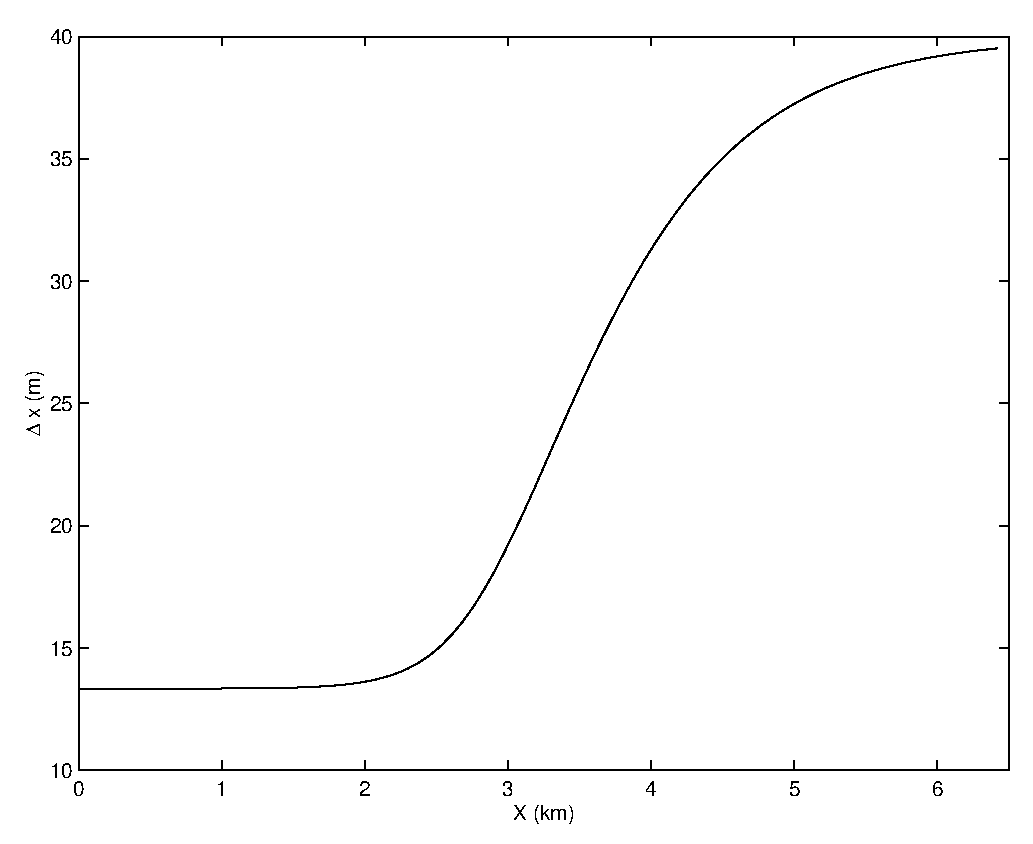
\includegraphics[width=\textwidth,height=.3\textheight]{s_examples/plume_on_slope/dx.eps}
\end{center}
\caption{Horizontal grid spacing, $\Delta x$, in the across-slope
direction for the gravity plume experiment.}
\label{fig:dx-plume-on-slope}
\end{figure}

\begin{figure}
\begin{center}
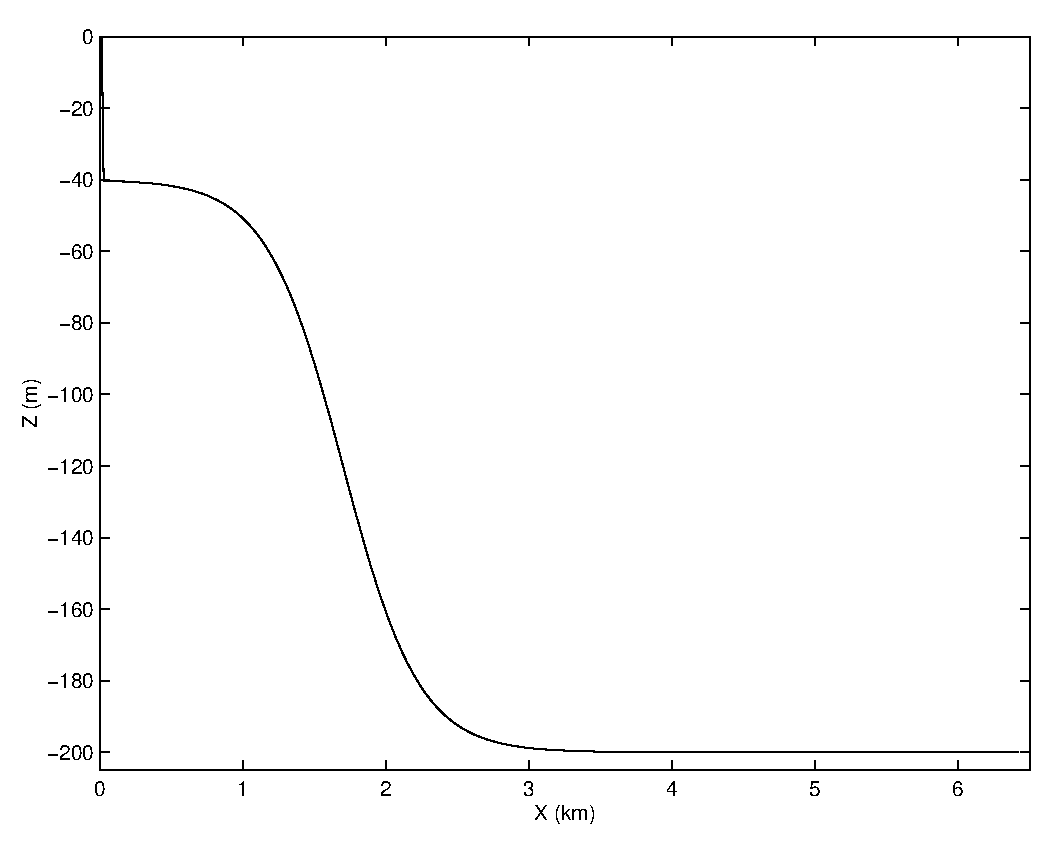
\includegraphics[width=\textwidth,height=.3\textheight]{s_examples/plume_on_slope/Depth.eps}
\end{center}
\caption{Topography, $h(x)$, used for the gravity plume experiment.}
\label{fig:depth-plume-on-slope}
\end{figure}

\begin{figure}
\begin{center}
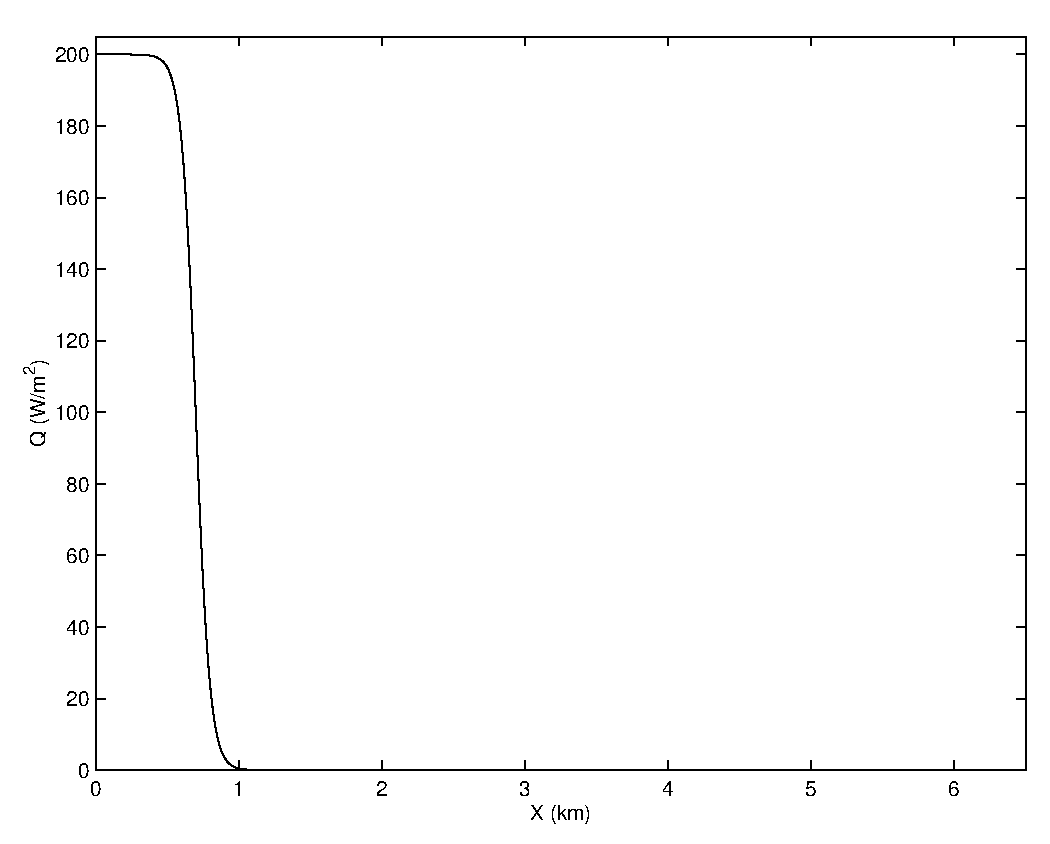
\includegraphics[width=\textwidth,height=.3\textheight]{s_examples/plume_on_slope/Qsurf.eps}
\end{center}
\caption{Upward surface heat flux, $Q(x)$, used as forcing in the
gravity plume experiment.}
\label{fig:Q-plume-on-slope}
\end{figure}

The domain is $200$~m deep and $6.4$~km across. Uniform resolution of
$60\times3^1/_3$~m is used in the vertical and variable resolution of
the form shown in Fig.~\ref{fig:dx-plume-on-slope} with $320$ points
is usedin the horizontal. The formula for $\Delta x$ is:
\begin{displaymath}
\Delta x(i) = \Delta x_1 + ( \Delta x_2 - \Delta x_1 )
( 1 + \tanh{\left(\frac{i-i_s}{w}\right)} ) /2
\end{displaymath}
where
\begin{eqnarray*}
Nx & = & 320 \\
Lx & = & 6400 \;\; \mbox{(m)} \\
\Delta x_1 & = & \frac{2}{3} \frac{Lx}{Nx} \;\; \mbox{(m)} \\
\Delta x_2 & = & \frac{Lx/2}{Nx-Lx/2 \Delta x_1} \;\; \mbox{(m)} \\
i_s & = & Lx/( 2 \Delta x_1 ) \\
w & = & 40 
\end{eqnarray*}
Here, $\Delta x_1$ is the resolution on the shelf, $\Delta x_2$ is the
resolution in deep water and $Nx$ is the number of points in the
horizontal.

The topography, shown in Fig.~\ref{fig:depth-plume-on-slope}, is given
by:
\begin{displaymath}
H(x) = -H_o + (H_o - h_s) ( 1 + \tanh{\left(\frac{x-x_s}{L_s}\right)} ) / 2
\end{displaymath}
where
\begin{eqnarray*}
H_o & = & 200 \;\; \mbox{(m)} \\
h_s & = & 40 \;\; \mbox{(m)} \\
x_s & = & 1500 + Lx/2 \;\; \mbox{(m)} \\
L_s & = & \frac{(H_o - h_s)}{2 s} \;\; \mbox{(m)} \\
s & = & 0.15
\end{eqnarray*}
Here, $s$ is the maximum slope, $H_o$ is the maximum depth, $h_s$ is
the shelf depth, $x_s$ is the lateral position of the shelf-break and
$L_s$ is the length-scale of the slope.

The forcing is through heat loss over the shelf, shown in
Fig.~\ref{fig:Q-plume-on-slope} and takes the form of a fixed flux
with profile:
\begin{displaymath}
Q(x) = Q_o ( 1 + \tanh{\left(\frac{x - x_q}{L_q}\right)} ) / 2
\end{displaymath}
where
\begin{eqnarray*}
Q_o & = & 200 \;\; \mbox{(W m$^{-2}$)} \\
x_q & = & 2500 + Lx/2 \;\; \mbox{(m)} \\
L_q & = & 100 \;\; \mbox{(m)}
\end{eqnarray*}
Here, $Q_o$, is the maximum heat flux, $x_q$ is the position of the
cut-off and $L_q$ is the width of the cut-off.

The initial tempeture field is unstratified but with random
perturbations, to induce convection early on in the run. The random
perturbation are calculated in computational space and because of the
variable resolution introduce some spatial correlations but this does
not matter for this experiment. The perturbations have range
$0-0.01$~$^{\circ}\mathrm{K}$.

\subsection{Code configuration}
\label{www:tutorials}
\label{sect:plume-config}

The computational domain (number of points) is specified in {\tt
code/SIZE.h} and is configured as a single tile of dimensions
$320\times1\times60$. There are no experiment specific source files.

Optional code required to for this experiment are the non-hydrostatic
algorithm and open-boundaries:
\begin{itemize}
\item Non-hydrostatic terms and algorithm are enabled with {\bf
\#define ALLOW\_NONHYDROSTATIC} in {\tt code/CPP\_OPTIONS.h} and
activated with {\bf nonHydrostatic=.TRUE.,} in namelist {\em PARM01}
of {\tt input/data}.
\item Open boundaries are enabled by adding line {\bf obcs} to 
package configuration file
{\tt code/packages.conf} and activated via {\bf useOBCS=.TRUE,} in
namelist {\em PACKAGES} of {\tt input/data.pkg}.
\end{itemize}

\subsection{Model parameters}
\label{www:tutorials}
\label{sect:plume-params}

\begin{table}
\begin{center}
\begin{tabular}{lll}
$g$ & $9.81$ m s$^{-2}$ & acceleration due to gravity \\
$\rho_o$ & $999.8$ kg m$^{-3}$ & reference density \\
$\alpha$ & $2 \times 10^{-4}$ K$^{-1}$ & expansion coefficient \\
$A_h$ & $1 \times 10^{-2}$ m$^2$s$^{-1}$ & horizontal viscosity \\
$A_v$ & $1 \times 10^{-3}$ m$^2$s$^{-1}$ & vertical viscosity \\
$\kappa_h$ & $0$ m$^2$s$^{-1}$ & (explicit) horizontal diffusion \\
$\kappa_v$ & $0$ m$^2$s$^{-1}$ & (explicit) vertical diffusion \\
\\
$\Delta t$ & $20$ s & time step \\
$\Delta z$ & $3.3\dot{3}$ m & vertical grid spacing \\
$\Delta x$ & $13.\dot{3}-39.5$ m & horizontal grid spacing
\end{tabular}
\end{center}
\caption{Model parameters used in the gravity plume experiment.}
\label{table:plume-on-slope}
\end{table}

The model parameters (Table~\ref{table:plume-on-slope}) are specified
in {\tt input/data} and if not assume the default values defined in
{\tt model/src/set\_defaults.F}. A linear equation of state is used,
{\bf eosType='LINEAR'}, but only temperature is active, {\bf
sBeta=0.E-4}. For the given heat flux, $Q_o$, the buoyancy forcing is
$B_o = \frac{g \alpha Q}{\rho_o c_p} \sim
10^{-7}$~m$^2$s$^{-3}$. Using $R=10^3$~m, the shelf width, then this
gives a velocity scale of $U\sim 5 \times 10^{-2}$~m~s$^-1$ for the
initial front but will accelerate by an order of magnitude over the
slope. The temperature anomaly will be of order $\Delta \theta \sim 3
\times 10^{-2}$~K.  The viscosity is constant and gives a Reynolds
number of $100$, using $h=20$~m for the initial front and will be an
order magnitude bigger over the slope. There is no explicit diffusion
but a non-linear advection scheme is used for temperature which adds
enough diffusion so as to keep the model stable. The time-step is set
to $20$~s and gives Courant number order one when the flow reaches the
bottom of the slope.

\subsection{Build and run the model}
\label{www:tutorials}

Build the model per usual. For example:
\begin{verbatim}
% cd verification/plume_on_slope
% mkdir build
% cd build
% ../../../tools/genmake -mods=../code -disable=gmredi,kpp,zonal_filt
  ,shap_filt
% make depend
% make
\end{verbatim}

When compilation is complete, run the model as usual, for example:
\begin{verbatim}
% cd ../
% mkdir run
% cp input/* build/mitgcmuv run/
% cd run
% ./mitgcmuv > output.txt
\end{verbatim}

\newpage
% $Header: /u/gcmpack/manual/s_examples/tracer_adjsens/Attic/co2sens.tex,v 1.9 2006/04/08 01:50:49 edhill Exp $
% $Name:  $

\section{Centennial Time Scale Tracer Injection}
\label{www:tutorials}
\label{sect:eg-simple-tracer}
\begin{rawhtml}
<!-- CMIREDIR:eg-simple-tracer: -->
\end{rawhtml}

\bodytext{bgcolor="#FFFFFFFF"}

%\begin{center} 
%{\Large \bf Using MITgcm to Look at Centennial Time Scale
%Sensitivities}
%
%\vspace*{4mm}
%
%\vspace*{3mm}
%{\large May 2001}
%\end{center}

\subsection{Introduction}
\label{www:tutorials}

This document describes the fourth example MITgcm experiment.
This example illustrates the use of
the MITgcm to perform sensitivity analysis in a
large scale ocean circulation simulation.

\subsection{Overview}
\label{www:tutorials}

This example experiment demonstrates using the MITgcm to simulate
the planetary ocean circulation. The simulation is configured
with realistic geography and bathymetry on a
$4^{\circ} \times 4^{\circ}$ spherical polar grid.
Twenty vertical layers are used in the vertical, ranging in thickness
from $50\,{\rm m}$ at the surface to $815\,{\rm m}$ at depth,
giving a maximum model depth of $6\,{\rm km}$.
At this resolution, the configuration
can be integrated forward for thousands of years on a single 
processor desktop computer.
\\

The model is forced with climatological wind stress data and surface
flux data from Da Silva \cite{DaSilva94}. Climatological data
from Levitus \cite{Levitus94} is used to initialize the model hydrography.
Levitus data is also used throughout the calculation
to derive air-sea fluxes of heat at the ocean surface.
These fluxes are combined with climatological estimates of
surface heat flux and fresh water, resulting in a mixed boundary
condition of the style described in Haney \cite{Haney}.
Altogether, this yields the following forcing applied
in the model surface layer.

\begin{eqnarray}
\label{EQ:eg-simple-tracer-global_forcing}
\label{EQ:eg-simple-tracer-global_forcing_fu}
{\cal F}_{u} & = & \frac{\tau_{x}}{\rho_{0} \Delta z_{s}}
\\
\label{EQ:eg-simple-tracer-global_forcing_fv}
{\cal F}_{v} & = & \frac{\tau_{y}}{\rho_{0} \Delta z_{s}}
\\
\label{EQ:eg-simple-tracer-global_forcing_ft}
{\cal F}_{\theta} & = & - \lambda_{\theta} ( \theta - \theta^{\ast} ) 
 - \frac{1}{C_{p} \rho_{0} \Delta z_{s}}{\cal Q}
\\
\label{EQ:eg-simple-tracer-global_forcing_fs}
{\cal F}_{s} & = & - \lambda_{s} ( S - S^{\ast} ) 
 + \frac{S_{0}}{\Delta z_{s}}({\cal E} - {\cal P} - {\cal R})
\end{eqnarray}

\noindent where ${\cal F}_{u}$, ${\cal F}_{v}$, ${\cal F}_{\theta}$,
${\cal F}_{s}$ are the forcing terms in the zonal and meridional
momentum and in the potential temperature and salinity 
equations respectively.
The term $\Delta z_{s}$ represents the top ocean layer thickness.
It is used in conjunction with the reference density, $\rho_{0}$
(here set to $999.8\,{\rm kg\,m^{-3}}$), the
reference salinity, $S_{0}$ (here set to 35ppt),
and a specific heat capacity $C_{p}$ to convert
wind-stress fluxes given in ${\rm N}\,m^{-2}$, 
\\


The configuration is illustrated in figure \ref{simulation_config}.


\subsection{Discrete Numerical Configuration}
\label{www:tutorials}


 The model is configured in hydrostatic form.  The domain is discretised with 
a uniform grid spacing in latitude and longitude of
 $\Delta x=\Delta y=4^{\circ}$, so 
that there are ninety grid cells in the $x$ and forty in the 
$y$ direction (Arctic polar regions are not
included in this experiment). Vertically the 
model is configured with twenty layers with the following thicknesses
$\Delta z_{1} = 50\,{\rm m},\,
 \Delta z_{2} = 50\,{\rm m},\,
 \Delta z_{3} = 55\,{\rm m},\,
 \Delta z_{4} = 60\,{\rm m},\,
 \Delta z_{5} = 65\,{\rm m},\,
$
$
 \Delta z_{6}~=~70\,{\rm m},\,
 \Delta z_{7}~=~80\,{\rm m},\,
 \Delta z_{8}~=95\,{\rm m},\,
 \Delta z_{9}=120\,{\rm m},\,
 \Delta z_{10}=155\,{\rm m},\,
$
$
 \Delta z_{11}=200\,{\rm m},\,
 \Delta z_{12}=260\,{\rm m},\,
 \Delta z_{13}=320\,{\rm m},\,
 \Delta z_{14}=400\,{\rm m},\,
 \Delta z_{15}=480\,{\rm m},\,
$
$
 \Delta z_{16}=570\,{\rm m},\,
 \Delta z_{17}=655\,{\rm m},\,
 \Delta z_{18}=725\,{\rm m},\,
 \Delta z_{19}=775\,{\rm m},\,
 \Delta z_{20}=815\,{\rm m}
$ (here the numeric subscript indicates the model level index number, ${\tt k}$).
The implicit free surface form of the pressure equation described in Marshall et. al 
\cite{marshall:97a} is employed. A Laplacian operator, $\nabla^2$, provides viscous
dissipation. Thermal and haline diffusion is also represented by a Laplacian operator.
\\

Wind-stress momentum inputs are added to the momentum equations for both
the zonal flow, $u$ and the meridional flow $v$, according to equations 
(\ref{EQ:eg-simple-tracer-global_forcing_fu}) and (\ref{EQ:eg-simple-tracer-global_forcing_fv}).
Thermodynamic forcing inputs are added to the equations for
potential temperature, $\theta$, and salinity, $S$, according to equations 
(\ref{EQ:eg-simple-tracer-global_forcing_ft}) and (\ref{EQ:eg-simple-tracer-global_forcing_fs}).
This produces a set of equations solved in this configuration as follows:
% {\fracktur}


\begin{eqnarray}
\label{EQ:eg-simple-tracer-model_equations}
\frac{Du}{Dt} - fv + 
  \frac{1}{\rho}\frac{\partial p^{'}}{\partial x} - 
  A_{h}\nabla_{h}^2u - A_{z}\frac{\partial^{2}u}{\partial z^{2}} 
& = &
{\cal F}_{u}
\\
\frac{Dv}{Dt} + fu + 
  \frac{1}{\rho}\frac{\partial p^{'}}{\partial y} - 
  A_{h}\nabla_{h}^2v - A_{z}\frac{\partial^{2}v}{\partial z^{2}} 
& = &
{\cal F}_{v}
\\
\frac{\partial \eta}{\partial t} + \nabla_{h}\cdot \vec{u}
&=&
0
\\
\frac{D\theta}{Dt} -
 K_{h}\nabla_{h}^2\theta  - \Gamma(K_{z})\frac{\partial^{2}\theta}{\partial z^{2}} 
& = &
{\cal F}_{\theta}
\\
\frac{D s}{Dt} -
 K_{h}\nabla_{h}^2 s  - \Gamma(K_{z})\frac{\partial^{2} s}{\partial z^{2}} 
& = &
{\cal F}_{s}
\\
g\rho_{0} \eta + \int^{0}_{-z}\rho^{'} dz & = & p^{'}
\\
\end{eqnarray}

\noindent where $u$ and $v$ are the $x$ and $y$ components of the
flow vector $\vec{u}$. The suffices ${s},{i}$ indicate surface and
interior model levels respectively. As described in
MITgcm Numerical Solution Procedure \ref{chap:discretization}, the time 
evolution of potential temperature, $\theta$, equation is solved prognostically.
The total pressure, $p$, is diagnosed by summing pressure due to surface 
elevation $\eta$ and the hydrostatic pressure.
\\

\subsubsection{Numerical Stability Criteria}
\label{www:tutorials}

The Laplacian dissipation coefficient, $A_{h}$, is set to $400 m s^{-1}$.
This value is chosen to yield a Munk layer width \cite{adcroft:95},

\begin{eqnarray}
\label{EQ:eg-simple-tracer-munk_layer}
M_{w} = \pi ( \frac { A_{h} }{ \beta } )^{\frac{1}{3}}
\end{eqnarray}

\noindent  of $\approx 100$km. This is greater than the model
resolution in mid-latitudes $\Delta x$, ensuring that the frictional 
boundary layer is well resolved.
\\

\noindent The model is stepped forward with a 
time step $\delta t=1200$secs. With this time step the stability 
parameter to the horizontal Laplacian friction \cite{adcroft:95}

\begin{eqnarray}
\label{EQ:eg-simple-tracer-laplacian_stability}
S_{l} = 4 \frac{A_{h} \delta t}{{\Delta x}^2}
\end{eqnarray}

\noindent evaluates to 0.012, which is well below the 0.3 upper limit
for stability. 
\\

\noindent The vertical dissipation coefficient, $A_{z}$, is set to 
$1\times10^{-2} {\rm m}^2{\rm s}^{-1}$. The associated stability limit

\begin{eqnarray}
\label{EQ:eg-simple-tracer-laplacian_stability_z}
S_{l} = 4 \frac{A_{z} \delta t}{{\Delta z}^2}
\end{eqnarray}

\noindent evaluates to $4.8 \times 10^{-5}$ which is again well below
the upper limit.
The values of $A_{h}$ and $A_{z}$ are also used for the horizontal ($K_{h}$) 
and vertical ($K_{z}$) diffusion coefficients for temperature respectively.
\\

\noindent The numerical stability for inertial oscillations
\cite{adcroft:95} 

\begin{eqnarray}
\label{EQ:eg-simple-tracer-inertial_stability}
S_{i} = f^{2} {\delta t}^2
\end{eqnarray}

\noindent evaluates to $0.0144$, which is well below the $0.5$ upper 
limit for stability.
\\

\noindent The advective CFL \cite{adcroft:95} for a extreme maximum 
horizontal flow
speed of $ | \vec{u} | = 2 ms^{-1}$

\begin{eqnarray}
\label{EQ:eg-simple-tracer-cfl_stability}
S_{a} = \frac{| \vec{u} | \delta t}{ \Delta x}
\end{eqnarray}

\noindent evaluates to $5 \times 10^{-2}$. This is well below the stability 
limit of 0.5.
\\

\noindent The stability parameter for internal gravity waves 
\cite{adcroft:95}

\begin{eqnarray}
\label{EQ:eg-simple-tracer-igw_stability}
S_{c} = \frac{c_{g} \delta t}{ \Delta x}
\end{eqnarray}

\noindent evaluates to $5 \times 10^{-2}$. This is well below the linear
stability limit of 0.25.
  
\subsection{Code Configuration}
\label{www:tutorials}
\label{SEC:code_config}

The model configuration for this experiment resides under the 
directory {\it verification/exp1/}.  The experiment files 
\begin{itemize}
\item {\it input/data}
\item {\it input/data.pkg}
\item {\it input/eedata},
\item {\it input/windx.sin\_y},
\item {\it input/topog.box},
\item {\it code/CPP\_EEOPTIONS.h}
\item {\it code/CPP\_OPTIONS.h},
\item {\it code/SIZE.h}. 
\end{itemize}
contain the code customizations and parameter settings for this 
experiments. Below we describe the customizations
to these files associated with this experiment.

\subsubsection{File {\it input/data}}
\label{www:tutorials}

This file, reproduced completely below, specifies the main parameters 
for the experiment. The parameters that are significant for this configuration
are

\begin{itemize}

\item Line 4, 
\begin{verbatim} tRef=20.,10.,8.,6., \end{verbatim} 
this line sets
the initial and reference values of potential temperature at each model
level in units of $^{\circ}\mathrm{C}$.
The entries are ordered from surface to depth. For each
depth level the initial and reference profiles will be uniform in
$x$ and $y$.

\fbox{
\begin{minipage}{5.0in}
{\it S/R INI\_THETA}({\it ini\_theta.F})
\end{minipage}
}


\item Line 6, 
\begin{verbatim} viscAz=1.E-2, \end{verbatim} 
this line sets the vertical Laplacian dissipation coefficient to
$1 \times 10^{-2} {\rm m^{2}s^{-1}}$. Boundary conditions
for this operator are specified later. This variable is copied into
model general vertical coordinate variable {\bf viscAr}.

\fbox{
\begin{minipage}{5.0in}
{\it S/R CALC\_DIFFUSIVITY}({\it calc\_diffusivity.F})
\end{minipage}
}

\item Line 7, 
\begin{verbatim}
viscAh=4.E2,
\end{verbatim} 
this line sets the horizontal Laplacian frictional dissipation coefficient to
$1 \times 10^{-2} {\rm m^{2}s^{-1}}$. Boundary conditions
for this operator are specified later.

\item Lines 8,
\begin{verbatim}
no_slip_sides=.FALSE.
\end{verbatim}
this line selects a free-slip lateral boundary condition for
the horizontal Laplacian friction operator 
e.g. $\frac{\partial u}{\partial y}$=0 along boundaries in $y$ and
$\frac{\partial v}{\partial x}$=0 along boundaries in $x$.

\item Lines 9,
\begin{verbatim}
no_slip_bottom=.TRUE.
\end{verbatim}
this line selects a no-slip boundary condition for bottom
boundary condition in the vertical Laplacian friction operator 
e.g. $u=v=0$ at $z=-H$, where $H$ is the local depth of the domain.

\item Line 10,
\begin{verbatim}
diffKhT=4.E2,
\end{verbatim}
this line sets the horizontal diffusion coefficient for temperature
to $400\,{\rm m^{2}s^{-1}}$. The boundary condition on this
operator is $\frac{\partial}{\partial x}=\frac{\partial}{\partial y}=0$ at
all boundaries.

\item Line 11,
\begin{verbatim}
diffKzT=1.E-2,
\end{verbatim}
this line sets the vertical diffusion coefficient for temperature
to $10^{-2}\,{\rm m^{2}s^{-1}}$. The boundary condition on this
operator is $\frac{\partial}{\partial z}$ = 0 on all boundaries.

\item Line 13,
\begin{verbatim}
tAlpha=2.E-4,
\end{verbatim}
This line sets the thermal expansion coefficient for the fluid
to $2 \times 10^{-4}\,{\rm degrees}^{-1}$

\fbox{
\begin{minipage}{5.0in}
{\it S/R FIND\_RHO}({\it find\_rho.F})
\end{minipage}
}

\item Line 18,
\begin{verbatim}
eosType='LINEAR'
\end{verbatim}
This line selects the linear form of the equation of state.

\fbox{
\begin{minipage}{5.0in}
{\it S/R FIND\_RHO}({\it find\_rho.F})
\end{minipage}
}



\item Line 40,
\begin{verbatim}
usingSphericalPolarGrid=.TRUE.,
\end{verbatim}
This line requests that the simulation be performed in a 
spherical polar coordinate system. It affects the interpretation of
grid input parameters, for example {\bf delX} and {\bf delY} and
causes the grid generation routines to initialize an internal grid based
on spherical polar geometry.

\fbox{
\begin{minipage}{5.0in}
{\it S/R INI\_SPEHRICAL\_POLAR\_GRID}({\it ini\_spherical\_polar\_grid.F})
\end{minipage}
}

\item Line 41,
\begin{verbatim}
phiMin=0.,
\end{verbatim}
This line sets the southern boundary of the modeled
domain to $0^{\circ}$ latitude. This value affects both the
generation of the locally orthogonal grid that the model
uses internally and affects the initialization of the coriolis force.
Note - it is not required to set
a longitude boundary, since the absolute longitude does
not alter the kernel equation discretisation.

\item Line 42,
\begin{verbatim}
delX=60*1.,
\end{verbatim}
This line sets the horizontal grid spacing between each y-coordinate line
in the discrete grid to $1^{\circ}$ in longitude.

\item Line 43,
\begin{verbatim}
delY=60*1.,
\end{verbatim}
This line sets the horizontal grid spacing between each y-coordinate line
in the discrete grid to $1^{\circ}$ in latitude.

\item Line 44,
\begin{verbatim}
delZ=500.,500.,500.,500.,
\end{verbatim}
This line sets the vertical grid spacing between each z-coordinate line
in the discrete grid to $500\,{\rm m}$, so that the total model depth 
is $2\,{\rm km}$. The variable {\bf delZ} is copied into the internal
model coordinate variable {\bf delR}

\fbox{
\begin{minipage}{5.0in}
{\it S/R INI\_VERTICAL\_GRID}({\it ini\_vertical\_grid.F})
\end{minipage}
}

\item Line 47,
\begin{verbatim}
bathyFile='topog.box'
\end{verbatim}
This line specifies the name of the file from which the domain
bathymetry is read. This file is a two-dimensional ($x,y$) map of
depths. This file is assumed to contain 64-bit binary numbers 
giving the depth of the model at each grid cell, ordered with the x 
coordinate varying fastest. The points are ordered from low coordinate
to high coordinate for both axes. The units and orientation of the
depths in this file are the same as used in the MITgcm code. In this
experiment, a depth of $0m$ indicates a solid wall and a depth
of $-2000m$ indicates open ocean. The matlab program
{\it input/gendata.m} shows an example of how to generate a
bathymetry file.


\item Line 50,
\begin{verbatim}
zonalWindFile='windx.sin_y'
\end{verbatim}
This line specifies the name of the file from which the x-direction
surface wind stress is read. This file is also a two-dimensional
($x,y$) map and is enumerated and formatted in the same manner as the 
bathymetry file. The matlab program {\it input/gendata.m} includes example 
code to generate a valid 
{\bf zonalWindFile} 
file.  

\end{itemize}

\noindent other lines in the file {\it input/data} are standard values
that are described in the MITgcm Getting Started and MITgcm Parameters
notes.

\begin{small}
% % $Header: /u/gcmpack/manual/s_examples/baroclinic_gyre/input/data.tex,v 1.1.1.1 2001/08/08 16:15:46 adcroft Exp $
% $Name:  $

\begin{verbatim}
     1	# Model parameters
     2	# Continuous equation parameters
     3	 &PARM01
     4	 tRef=20.,10.,8.,6.,
     5	 sRef=10.,10.,10.,10.,
     6	 viscAz=1.E-2,
     7	 viscAh=4.E2,
     8	 no_slip_sides=.FALSE.,
     9	 no_slip_bottom=.TRUE.,
    10	 diffKhT=4.E2,
    11	 diffKzT=1.E-2,
    12	 beta=1.E-11,
    13	 tAlpha=2.E-4,
    14	 sBeta =0.,
    15	 gravity=9.81,
    16	 rigidLid=.FALSE.,
    17	 implicitFreeSurface=.TRUE.,
    18	 eosType='LINEAR',
    19	 readBinaryPrec=64,
    20	 &
    21	# Elliptic solver parameters
    22	 &PARM02
    23	 cg2dMaxIters=1000,
    24	 cg2dTargetResidual=1.E-13,
    25	 &
    26	# Time stepping parameters
    27	 &PARM03
    28	 startTime=0.,
    29	 endTime=12000., 
    30	 deltaTmom=1200.0,
    31	 deltaTtracer=1200.0,
    32	 abEps=0.1,
    33	 pChkptFreq=17000.0,
    34	 chkptFreq=0.0,
    35	 dumpFreq=2592000.0,
    36	 &
    37	# Gridding parameters
    38	 &PARM04
    39	 usingCartesianGrid=.FALSE.,
    40	 usingSphericalPolarGrid=.TRUE.,
    41	 phiMin=0.,
    42	 delX=60*1.,
    43	 delY=60*1.,
    44	 delZ=500.,500.,500.,500.,
    45	 &
    46	 &PARM05
    47	 bathyFile='topog.box',
    48	 hydrogThetaFile=,
    49	 hydrogSaltFile=,
    50	 zonalWindFile='windx.sin_y',
    51	 meridWindFile=,
    52	 &
\end{verbatim}

\end{small}

\subsubsection{File {\it input/data.pkg}}
\label{www:tutorials}

This file uses standard default values and does not contain
customizations for this experiment.

\subsubsection{File {\it input/eedata}}
\label{www:tutorials}

This file uses standard default values and does not contain
customizations for this experiment.

\subsubsection{File {\it input/windx.sin\_y}}
\label{www:tutorials}

The {\it input/windx.sin\_y} file specifies a two-dimensional ($x,y$) 
map of wind stress ,$\tau_{x}$, values. The units used are $Nm^{-2}$.
Although $\tau_{x}$ is only a function of $y$n in this experiment
this file must still define a complete two-dimensional map in order
to be compatible with the standard code for loading forcing fields 
in MITgcm. The included matlab program {\it input/gendata.m} gives a complete
code for creating the {\it input/windx.sin\_y} file.

\subsubsection{File {\it input/topog.box}}
\label{www:tutorials}


The {\it input/topog.box} file specifies a two-dimensional ($x,y$) 
map of depth values. For this experiment values are either
$0m$ or $-2000\,{\rm m}$, corresponding respectively to a wall or to deep
ocean. The file contains a raw binary stream of data that is enumerated
in the same way as standard MITgcm two-dimensional, horizontal arrays.
The included matlab program {\it input/gendata.m} gives a complete
code for creating the {\it input/topog.box} file.

\subsubsection{File {\it code/SIZE.h}}
\label{www:tutorials}

Two lines are customized in this file for the current experiment

\begin{itemize}

\item Line 39, 
\begin{verbatim} sNx=60, \end{verbatim} this line sets
the lateral domain extent in grid points for the
axis aligned with the x-coordinate.

\item Line 40, 
\begin{verbatim} sNy=60, \end{verbatim} this line sets
the lateral domain extent in grid points for the
axis aligned with the y-coordinate.

\item Line 49, 
\begin{verbatim} Nr=4,   \end{verbatim} this line sets
the vertical domain extent in grid points.

\end{itemize}

\begin{small}
% \begin{verbatim}
     1	C     /==========================================================\
     2	C     | SIZE.h Declare size of underlying computational grid.    |
     3	C     |==========================================================|
     4	C     | The design here support a three-dimensional model grid   |
     5	C     | with indices I,J and K. The three-dimensional domain     |
     6	C     | is comprised of nPx*nSx blocks of size sNx along one axis|
     7	C     | nPy*nSy blocks of size sNy along another axis and one    |
     8	C     | block of size Nz along the final axis.                   |
     9	C     | Blocks have overlap regions of size OLx and OLy along the|
    10	C     | dimensions that are subdivided.                          |
    11  C     \==========================================================/
    12  C     Voodoo numbers controlling data layout.
    13  C     sNx - No. X points in sub-grid.
    14  C     sNy - No. Y points in sub-grid.
    15  C     OLx - Overlap extent in X.
    16  C     OLy - Overlat extent in Y.
    17  C     nSx - No. sub-grids in X.
    18  C     nSy - No. sub-grids in Y.
    19  C     nPx - No. of processes to use in X.
    20  C     nPy - No. of processes to use in Y.
    21  C     Nx  - No. points in X for the total domain.
    22  C     Ny  - No. points in Y for the total domain.
    23  C     Nr  - No. points in Z for full process domain.
    24        INTEGER sNx
    25        INTEGER sNy
    26        INTEGER OLx
    27        INTEGER OLy
    28        INTEGER nSx
    29        INTEGER nSy
    30        INTEGER nPx
    31	      INTEGER nPy
    32	      INTEGER Nx
    33	      INTEGER Ny
    34	      INTEGER Nr
    35	      PARAMETER (
    36	     &           sNx =  64,
    37	     &           sNy =  64,
    38	     &           OLx =   3,
    39	     &           OLy =   3,
    40	     &           nSx =   1,
    41	     &           nSy =   1,
    42	     &           nPx =   1,
    43	     &           nPy =   1,
    44	     &           Nx  = sNx*nSx*nPx,
    45	     &           Ny  = sNy*nSy*nPy,
    46	     &           Nr  =  20)

    47	C     MAX_OLX  - Set to the maximum overlap region size of any array
    48	C     MAX_OLY    that will be exchanged. Controls the sizing of exch
    49	C                routine buufers.
    50	      INTEGER MAX_OLX
    51	      INTEGER MAX_OLY
    52	      PARAMETER ( MAX_OLX = OLx,
    53	     &            MAX_OLY = OLy )

\end{verbatim}
\end{small}

\subsubsection{File {\it code/CPP\_OPTIONS.h}}
\label{www:tutorials}

This file uses standard default values and does not contain
customizations for this experiment.


\subsubsection{File {\it code/CPP\_EEOPTIONS.h}}
\label{www:tutorials}

This file uses standard default values and does not contain
customizations for this experiment.

\subsubsection{Other Files }
\label{www:tutorials}

Other files relevant to this experiment are
\begin{itemize}
\item {\it model/src/ini\_cori.F}. This file initializes the model
coriolis variables {\bf fCorU}.
\item {\it model/src/ini\_spherical\_polar\_grid.F}
\item {\it model/src/ini\_parms.F},
\item {\it input/windx.sin\_y},
\end{itemize}
contain the code customizations and parameter settings for this 
experiments. Below we describe the customizations
to these files associated with this experiment.

